%% Supplementary Material to "ABS challenges: an accounting index of wins left on the table".
%% Every number is a macro from generated/numbers.tex or a table from generated/tab_s_*.tex (paper/make_numbers.py and
%% paper/supplement_numbers.py read results/); references to the main text are \Mref{label}, written by paper/xrefs.py from main.aux. Build: make -C paper.
\documentclass[aoas]{imsart}

\RequirePackage{amsthm,amsmath,amsfonts,amssymb}
\RequirePackage[authoryear]{natbib}
\RequirePackage{xurl}
\RequirePackage[colorlinks,citecolor=blue,urlcolor=blue,pdftitle={Supplement to ABS challenges: an accounting index of wins left on the table},
  pdfauthor={Jan Janou\v{s}ek and Michal Pe\v{s}ta}]{hyperref}
\RequirePackage{graphicx,booktabs}
\RequirePackage[section]{placeins}

\startlocaldefs
\theoremstyle{plain}
\newtheorem{theorem}{Theorem}
\newtheorem{proposition}[theorem]{Proposition}
\newtheorem{lemma}[theorem]{Lemma}
\theoremstyle{definition}
\newtheorem{remark}{Remark}
\newcommand{\E}{\mathbb{E}}
\newcommand{\Prob}{\mathbb{P}}
\newenvironment{restate}[1]{\par\medskip\noindent\textbf{#1 (main text).}\ \itshape}{\par\medskip}
\newcommand{\status}[1]{\textup{[\textsc{#1}]}}
\newcommand{\tstatus}[1]{\textup{\textsc{#1}}}
\renewcommand{\thesection}{S\arabic{section}}
\renewcommand{\thetheorem}{S\arabic{theorem}}
\renewcommand{\theremark}{S\arabic{remark}}
\renewcommand{\theequation}{S\arabic{equation}}
\renewcommand{\thetable}{S\arabic{table}}
\renewcommand{\thefigure}{S\arabic{figure}}
\setcounter{secnumdepth}{3}
% generated by paper/make_numbers.py from results/ -- do not edit
\newcommand{\AAASrBatter}{3.22}
\newcommand{\AAASrCatcher}{2.09}
\newcommand{\AAASrPctHi}{15}
\newcommand{\AAASrPctLo}{12}
\newcommand{\BGTopChExcess}{25}
\newcommand{\BGTopValueExcess}{0.02}
\newcommand{\BGValueExpected}{3.32}
\newcommand{\BGValueObserved}{3.34}
\newcommand{\BICMain}{55{,}329}
\newcommand{\BICRE}{54{,}049}
\newcommand{\BICRELapse}{54{,}035}
\newcommand{\BICSmoothMinusDet}{58}
\newcommand{\BinaryLost}{0.68}
\newcommand{\BinaryLostCI}{[0.57, 0.80]}
\newcommand{\BinaryMinusRB}{\ensuremath{-}0.008}
\newcommand{\BinaryMinusRBCI}{[\ensuremath{-}0.025, 0.009]}
\newcommand{\BinaryMinusRBSimAbs}{0.00}
\newcommand{\BlockBootB}{100}
\newcommand{\BlockBootCI}{[0.54, 0.78]}
\newcommand{\BreakEvenLLBatter}{73}
\newcommand{\BreakEvenLLCatcher}{133}
\newcommand{\BreakEvenPct}{20}
\newcommand{\CIEndSE}{0.008}
\newcommand{\CPLapseB}{50}
\newcommand{\CPLapseBasic}{17}
\newcommand{\CPLapseBias}{0.162}
\newcommand{\CPLapseBiasK}{0.212}
\newcommand{\CPLapseBiasSE}{0.010}
\newcommand{\CPLapseBootSD}{0.064}
\newcommand{\CPLapseGap}{0.57}
\newcommand{\CPLapseGapK}{0.52}
\newcommand{\CPLapseKBasic}{7}
\newcommand{\CPLapseKNormal}{10}
\newcommand{\CPLapseKPct}{10}
\newcommand{\CPLapseKPctCI}{[2, 27]}
\newcommand{\CPLapseLearn}{0.05}
\newcommand{\CPLapseMissHigh}{21}
\newcommand{\CPLapseMissLow}{0}
\newcommand{\CPLapseNormal}{23}
\newcommand{\CPLapsePct}{30}
\newcommand{\CPLapsePctCI}{[15, 49]}
\newcommand{\CPLapsePointSD}{0.055}
\newcommand{\CPLapseS}{30}
\newcommand{\CPMainB}{50}
\newcommand{\CPMainBasic}{90}
\newcommand{\CPMainBias}{\ensuremath{-}0.037}
\newcommand{\CPMainBiasK}{\ensuremath{-}0.032}
\newcommand{\CPMainBiasSE}{0.008}
\newcommand{\CPMainBootSD}{0.064}
\newcommand{\CPMainGap}{0.70}
\newcommand{\CPMainGapK}{0.69}
\newcommand{\CPMainKBasic}{88}
\newcommand{\CPMainKNormal}{90}
\newcommand{\CPMainKPct}{92}
\newcommand{\CPMainKPctCI}{[81, 98]}
\newcommand{\CPMainLearn}{0.01}
\newcommand{\CPMainMissHigh}{0}
\newcommand{\CPMainMissLow}{4}
\newcommand{\CPMainNormal}{90}
\newcommand{\CPMainPct}{92}
\newcommand{\CPMainPctCI}{[81, 98]}
\newcommand{\CPMainPointSD}{0.055}
\newcommand{\CPMainS}{50}
\newcommand{\CPMisB}{20}
\newcommand{\CPMisBasic}{50}
\newcommand{\CPMisBias}{\ensuremath{-}0.072}
\newcommand{\CPMisBiasK}{\ensuremath{-}0.001}
\newcommand{\CPMisBiasSE}{0.012}
\newcommand{\CPMisBootSD}{0.066}
\newcommand{\CPMisGap}{0.78}
\newcommand{\CPMisGapK}{0.71}
\newcommand{\CPMisKBasic}{92}
\newcommand{\CPMisKNormal}{100}
\newcommand{\CPMisKPct}{92}
\newcommand{\CPMisKPctCI}{[62, 100]}
\newcommand{\CPMisLearn}{0.07}
\newcommand{\CPMisMissHigh}{0}
\newcommand{\CPMisMissLow}{0}
\newcommand{\CPMisNormal}{92}
\newcommand{\CPMisPct}{100}
\newcommand{\CPMisPctCI}{[74, 100]}
\newcommand{\CPMisPointSD}{0.040}
\newcommand{\CPMisS}{12}
\newcommand{\CPPrimB}{30}
\newcommand{\CPPrimBasic}{50}
\newcommand{\CPPrimBias}{\ensuremath{-}0.069}
\newcommand{\CPPrimBiasK}{0.009}
\newcommand{\CPPrimBiasSE}{0.011}
\newcommand{\CPPrimBootSD}{0.063}
\newcommand{\CPPrimGap}{0.65}
\newcommand{\CPPrimGapK}{0.57}
\newcommand{\CPPrimKBasic}{80}
\newcommand{\CPPrimKNormal}{100}
\newcommand{\CPPrimKPct}{80}
\newcommand{\CPPrimKPctCI}{[61, 92]}
\newcommand{\CPPrimLearn}{0.08}
\newcommand{\CPPrimMissHigh}{0}
\newcommand{\CPPrimMissLow}{4}
\newcommand{\CPPrimNormal}{77}
\newcommand{\CPPrimPct}{87}
\newcommand{\CPPrimPctCI}{[69, 96]}
\newcommand{\CPPrimPointSD}{0.061}
\newcommand{\CPPrimS}{30}
\newcommand{\CPREB}{50}
\newcommand{\CPREBasic}{43}
\newcommand{\CPREBias}{0.095}
\newcommand{\CPREBiasK}{0.160}
\newcommand{\CPREBiasSE}{0.009}
\newcommand{\CPREBootSD}{0.064}
\newcommand{\CPREGap}{0.65}
\newcommand{\CPREGapK}{0.58}
\newcommand{\CPREKBasic}{23}
\newcommand{\CPREKNormal}{27}
\newcommand{\CPREKPct}{37}
\newcommand{\CPREKPctCI}{[20, 56]}
\newcommand{\CPRELearn}{0.07}
\newcommand{\CPREMissHigh}{4}
\newcommand{\CPREMissLow}{0}
\newcommand{\CPRENormal}{70}
\newcommand{\CPREPct}{87}
\newcommand{\CPREPctCI}{[69, 96]}
\newcommand{\CPREPointSD}{0.052}
\newcommand{\CPRES}{30}
\newcommand{\CausalBootN}{2{,}000}
\newcommand{\CausalK}{1000}
\newcommand{\CausalMinusPath}{0.000}
\newcommand{\CausalMinusPathCI}{[\ensuremath{-}0.002, 0.002]}
\newcommand{\CausalR}{10}
\newcommand{\CausalSkipShare}{47}
\newcommand{\ClairGap}{0.81}
\newcommand{\CoB}{400}
\newcommand{\CoLost}{0.55}
\newcommand{\CoLostCI}{[0.36, 0.72]}
\newcommand{\CoLostRemoved}{0.91}
\newcommand{\CoShareRule}{95.4}
\newcommand{\ContamPct}{0.05}
\newcommand{\CovB}{20}
\newcommand{\CovBMis}{10}
\newcommand{\CovBootSD}{0.071}
\newcommand{\CovGap}{0.72}
\newcommand{\CovLapseBias}{0.15}
\newcommand{\CovLapseGap}{0.60}
\newcommand{\CovLapseNormal}{45}
\newcommand{\CovLapseRate}{32}
\newcommand{\CovLapseS}{22}
\newcommand{\CovMainBasic}{80}
\newcommand{\CovMainBias}{\ensuremath{-}0.055}
\newcommand{\CovMainBiasAbs}{0.06}
\newcommand{\CovMainMissHigh}{0}
\newcommand{\CovMainMissLow}{10}
\newcommand{\CovMainNormal}{90}
\newcommand{\CovMainRate}{80}
\newcommand{\CovMainRateCI}{[66.3, 90.0]}
\newcommand{\CovPointSD}{0.061}
\newcommand{\CovR}{2}
\newcommand{\CovREBias}{0.06}
\newcommand{\CovREGap}{0.68}
\newcommand{\CovRENormal}{85}
\newcommand{\CovRERate}{73}
\newcommand{\CovRES}{26}
\newcommand{\CovS}{50}
\newcommand{\CovSMis}{30}
\newcommand{\CovTruthStreams}{16}
\newcommand{\CrossFive}{27}
\newcommand{\CrossThree}{10}
\newcommand{\CrossTwo}{4}
\newcommand{\CurseBias}{0.07}
\newcommand{\CurseBiasSD}{0.01}
\newcommand{\CurseLostCross}{0.65}
\newcommand{\CurseLostSame}{0.72}
\newcommand{\DLLEdge}{193}
\newcommand{\DLLMain}{355}
\newcommand{\DLLRE}{1{,}032}
\newcommand{\DLLREvsMain}{679}
\newcommand{\DLLRejHi}{854}
\newcommand{\DLLRejLo}{107}
\newcommand{\DLLRejMainHi}{893}
\newcommand{\DLLRejMainLo}{126}
\newcommand{\DPConcEntPct}{0.6}
\newcommand{\DPConcOppPct}{0.1}
\newcommand{\DPRiseEntPct}{20}
\newcommand{\DPRiseOppPct}{9}
\newcommand{\DRSB}{500}
\newcommand{\DRSMatches}{2{,}279}
\newcommand{\DRSODILBW}{29.0}
\newcommand{\DRSODILost}{0.018}
\newcommand{\DRSODILostObs}{0.00}
\newcommand{\DRSODILostObsCI}{[\ensuremath{-}0.13, 0.44]}
\newcommand{\DRSODIMove}{13}
\newcommand{\DRSODIPower}{1.67}
\newcommand{\DRSODIS}{0.81}
\newcommand{\DRSODIShare}{98.5}
\newcommand{\DRSTestLBW}{30.3}
\newcommand{\DRSTestLost}{0.020}
\newcommand{\DRSTestLostObs}{0.13}
\newcommand{\DRSTestLostObsCI}{[\ensuremath{-}0.27, 0.49]}
\newcommand{\DRSTestMove}{18}
\newcommand{\DRSTestPower}{1.66}
\newcommand{\DRSTestS}{0.47}
\newcommand{\DRSTestShare}{99.8}
\newcommand{\DRSTtLBW}{27.8}
\newcommand{\DRSTtLost}{0.001}
\newcommand{\DRSTtLostObs}{0.02}
\newcommand{\DRSTtLostObsCI}{[\ensuremath{-}0.04, 0.09]}
\newcommand{\DRSTtMove}{7}
\newcommand{\DRSTtPower}{1.85}
\newcommand{\DRSTtS}{0.45}
\newcommand{\DRSTtShare}{99.5}
\newcommand{\DecBothGap}{82}
\newcommand{\DecBothGapCI}{[71, 86]}
\newcommand{\DecBothN}{2.39}
\newcommand{\DecBothScaleGap}{79}
\newcommand{\DecBothScaleN}{2.53}
\newcommand{\DecBothScaleShare}{96.5}
\newcommand{\DecBothShare}{96.9}
\newcommand{\DecFitGap}{-6}
\newcommand{\DecFitN}{2.15}
\newcommand{\DecFitShare}{82.4}
\newcommand{\DecIntGap}{53}
\newcommand{\DecIntGapCI}{[38, 61]}
\newcommand{\DecIntN}{2.93}
\newcommand{\DecIntShare}{92.1}
\newcommand{\DecR}{20}
\newcommand{\DecRTune}{10}
\newcommand{\DecStakeBeatsPct}{100}
\newcommand{\DecStakeGap}{81}
\newcommand{\DecStakeGapCI}{[68, 87]}
\newcommand{\DecStakeN}{2.45}
\newcommand{\DecStakeScaleGap}{69}
\newcommand{\DecStakeScaleGapCI}{[59, 80]}
\newcommand{\DecStakeScaleN}{2.33}
\newcommand{\DecStakeScaleShare}{94.9}
\newcommand{\DecStakeShare}{96.9}
\newcommand{\DeltaFirst}{0.017}
\newcommand{\DeltaRatio}{0.53--0.54}
\newcommand{\DeltaSqRTwoAway}{0.9975}
\newcommand{\DeltaSqRTwoHome}{0.9976}
\newcommand{\DetCoordBiasBatter}{0.5}
\newcommand{\DetCoordBiasCatcher}{1.4}
\newcommand{\DetRank}{2}
\newcommand{\DetVersion}{15.0}
\newcommand{\EdgeOrigSlope}{0.84}
\newcommand{\EdgeOrigSlopeCI}{[0.59, 1.09]}
\newcommand{\EdgeOtherSDMax}{0.09}
\newcommand{\EdgeStrikesSD}{0.28}
\newcommand{\ExtraGamesPct}{9}
\newcommand{\FMDeltaCI}{[0.008, 0.009]}
\newcommand{\FMGapClosed}{68}
\newcommand{\FMGapClosedCI}{[61, 75]}
\newcommand{\FarLogGBatter}{0.34}
\newcommand{\FarLogGCatcher}{0.39}
\newcommand{\FarLogGSEBatter}{0.13}
\newcommand{\FarLogGSECatcher}{0.22}
\newcommand{\FarNBatter}{374}
\newcommand{\FarNCatcher}{241}
\newcommand{\FarOneLeftBatter}{\ensuremath{-}0.74}
\newcommand{\FarOneLeftCatcher}{\ensuremath{-}0.92}
\newcommand{\FarOneLeftSEBatter}{0.26}
\newcommand{\FarOneLeftSECatcher}{0.35}
\newcommand{\FarRateBatter}{44}
\newcommand{\FarRateCatcher}{70}
\newcommand{\FarRateOneBatter}{38}
\newcommand{\FarRateOneCatcher}{61}
\newcommand{\FarRateTwoBatter}{46}
\newcommand{\FarRateTwoCatcher}{74}
\newcommand{\FeedBaseSrBatter}{3.11}
\newcommand{\FeedBaseSrCatcher}{1.88}
\newcommand{\FeedSrBatter}{2.90}
\newcommand{\FeedSrCatcher}{1.84}
\newcommand{\FlatBestDelta}{0.008}
\newcommand{\FlatBound}{44.7}
\newcommand{\FlatIdentityGap}{6\times 10^{-17}}
\newcommand{\FlatLocal}{6.5}
\newcommand{\FlatLoss}{6.0}
\newcommand{\FrozenAllDelta}{0.008}
\newcommand{\FrozenDPShare}{99.1}
\newcommand{\FrozenDPShareNoEng}{99.2}
\newcommand{\FrozenDPShareWorldTest}{98.4}
\newcommand{\FrozenDelta}{0.008}
\newcommand{\FrozenGapClosed}{68}
\newcommand{\FrozenLost}{0.48}
\newcommand{\FrozenLostNoEng}{0.48}
\newcommand{\FrozenLostWorldTest}{0.60}
\newcommand{\FrozenR}{20}
\newcommand{\FrozenRuleGapClosed}{64}
\newcommand{\FrozenRuleShareDP}{95.6}
\newcommand{\FrozenRuleShareRetro}{94.7}
\newcommand{\FrozenRuleShareRetroNoEng}{94.7}
\newcommand{\FrozenRuleShareRetroWorldTest}{94.4}
\newcommand{\FrozenShare}{95.7}
\newcommand{\FrozenTestGames}{1{,}146}
\newcommand{\FrozenTrainGames}{1{,}279}
\newcommand{\FullPathObs}{0.69}
\newcommand{\FullPathRule}{0.72}
\newcommand{\FullRB}{0.72}
\newcommand{\FullRBCI}{[0.65, 0.79]}
\newcommand{\FullWin}{0.70}
\newcommand{\FullWinCI}{[0.63, 0.77]}
\newcommand{\Gap}{0.51}
\newcommand{\GapAlgPct}{12}
\newcommand{\GapB}{400}
\newcommand{\GapBFail}{0}
\newcommand{\GapBFailDiff}{0.000}
\newcommand{\GapBFailText}{all fold fits reached the gradient tolerance}
\newcommand{\GapBasic}{[0.35, 0.61]}
\newcommand{\GapBench}{3.85}
\newcommand{\GapBenchCI}{[3.71, 4.06]}
\newcommand{\GapBestDelta}{0.007}
\newcommand{\GapBestShare}{95.5}
\newcommand{\GapBootBias}{0.027}
\newcommand{\GapBootHours}{915}
\newcommand{\GapBootMean}{0.53}
\newcommand{\GapBootMinutes}{137}
\newcommand{\GapBootSD}{0.064}
\newcommand{\GapBootSDAlg}{0.060}
\newcommand{\GapCI}{[0.38, 0.63]}
\newcommand{\GapCalFine}{0.39}
\newcommand{\GapCalFineNauxEight}{0.44}
\newcommand{\GapCardPubGapPct}{60}
\newcommand{\GapCardPubN}{2.54}
\newcommand{\GapCardPubShare}{94.8}
\newcommand{\GapCardRefitGapPct}{56}
\newcommand{\GapCardRefitN}{2.55}
\newcommand{\GapCardRefitShare}{94.2}
\newcommand{\GapDTrainHi}{0.0077}
\newcommand{\GapDTrainLo}{0.0069}
\newcommand{\GapEarlyLateOne}{8.5}
\newcommand{\GapEarlyLateOneCI}{[7.1, 9.8]}
\newcommand{\GapEarlyLateOneDown}{27.3}
\newcommand{\GapEarlyLateOneOcc}{27.5}
\newcommand{\GapEarlyLateOneOccCI}{[26.6, 28.7]}
\newcommand{\GapEarlyLateOneUp}{27.3}
\newcommand{\GapEarlyLateTwo}{12.5}
\newcommand{\GapEarlyLateTwoCI}{[11.5, 13.4]}
\newcommand{\GapEarlyLateTwoDown}{27.7}
\newcommand{\GapEarlyLateTwoOcc}{27.0}
\newcommand{\GapEarlyLateTwoOccCI}{[26.3, 27.7]}
\newcommand{\GapEarlyLateTwoUp}{29.6}
\newcommand{\GapExtS}{8}
\newcommand{\GapFMGapCI}{[53, 72]}
\newcommand{\GapFMGapPct}{63}
\newcommand{\GapFitRuleCI}{[\ensuremath{-}44.7, \ensuremath{-}0.2]}
\newcommand{\GapFitRuleGapPct}{\ensuremath{-}16}
\newcommand{\GapFitRuleN}{2.16}
\newcommand{\GapFitRuleShare}{84.7}
\newcommand{\GapFitRuleWins}{3.26}
\newcommand{\GapFrozenGapCI}{[54, 73]}
\newcommand{\GapFrozenGapPct}{64}
\newcommand{\GapFrozenN}{2.27}
\newcommand{\GapFrozenShare}{95.3}
\newcommand{\GapFrozenWins}{3.67}
\newcommand{\GapGridHi}{2.93}
\newcommand{\GapK}{5}
\newcommand{\GapLamHalf}{0.68}
\newcommand{\GapLamOne}{0.85}
\newcommand{\GapLapse}{0.46}
\newcommand{\GapLeague}{15}
\newcommand{\GapMCSE}{0.013}
\newcommand{\GapMain}{0.63}
\newcommand{\GapMainAlgPct}{9}
\newcommand{\GapMainB}{400}
\newcommand{\GapMainBFail}{22}
\newcommand{\GapMainBFailDiff}{0.002}
\newcommand{\GapMainBFailText}{22 replicates with a fold that did not are kept}
\newcommand{\GapMainBasic}{[0.53, 0.79]}
\newcommand{\GapMainBench}{3.98}
\newcommand{\GapMainBenchCI}{[3.79, 4.11]}
\newcommand{\GapMainBestDelta}{0.008}
\newcommand{\GapMainBestShare}{95.3}
\newcommand{\GapMainBootBias}{\ensuremath{-}0.026}
\newcommand{\GapMainBootHours}{17}
\newcommand{\GapMainBootMean}{0.61}
\newcommand{\GapMainBootMinutes}{3}
\newcommand{\GapMainBootSD}{0.063}
\newcommand{\GapMainBootSDAlg}{0.060}
\newcommand{\GapMainCI}{[0.51, 0.76]}
\newcommand{\GapMainCalFine}{0.60}
\newcommand{\GapMainCardPubGapPct}{65}
\newcommand{\GapMainCardPubN}{2.59}
\newcommand{\GapMainCardPubShare}{94.4}
\newcommand{\GapMainCardRefitGapPct}{58}
\newcommand{\GapMainCardRefitN}{2.51}
\newcommand{\GapMainCardRefitShare}{93.3}
\newcommand{\GapMainDTrainHi}{0.0081}
\newcommand{\GapMainDTrainLo}{0.0075}
\newcommand{\GapMainExtS}{8}
\newcommand{\GapMainFMGapCI}{[60, 75]}
\newcommand{\GapMainFMGapPct}{69}
\newcommand{\GapMainFitRuleCI}{[\ensuremath{-}29.6, 5.6]}
\newcommand{\GapMainFitRuleGapPct}{\ensuremath{-}7}
\newcommand{\GapMainFitRuleN}{2.16}
\newcommand{\GapMainFitRuleShare}{83.0}
\newcommand{\GapMainFitRuleWins}{3.30}
\newcommand{\GapMainFrozenGapCI}{[59, 75]}
\newcommand{\GapMainFrozenGapPct}{69}
\newcommand{\GapMainFrozenN}{2.25}
\newcommand{\GapMainFrozenShare}{95.1}
\newcommand{\GapMainFrozenWins}{3.78}
\newcommand{\GapMainGridHi}{2.68}
\newcommand{\GapMainK}{5}
\newcommand{\GapMainKTen}{0.67}
\newcommand{\GapMainKTwo}{0.61}
\newcommand{\GapMainLeague}{19}
\newcommand{\GapMainMCSE}{0.012}
\newcommand{\GapMainNBench}{2.70}
\newcommand{\GapMainNMorePct}{24}
\newcommand{\GapMainNObs}{2.18}
\newcommand{\GapMainNormal}{[0.51, 0.76]}
\newcommand{\GapMainObs}{3.34}
\newcommand{\GapMainObsCI}{[3.17, 3.51]}
\newcommand{\GapMainObsShare}{84.1}
\newcommand{\GapMainPct}{[0.48, 0.73]}
\newcommand{\GapMainR}{16}
\newcommand{\GapMainRefits}{2{,}000}
\newcommand{\GapMainRetuneBothGapPct}{79}
\newcommand{\GapMainRetuneBothN}{2.47}
\newcommand{\GapMainRetuneBothShare}{96.6}
\newcommand{\GapMainRetuneIntGapPct}{50}
\newcommand{\GapMainRetuneIntN}{3.03}
\newcommand{\GapMainRetuneIntShare}{92.0}
\newcommand{\GapMainRetuneSlopeGapPct}{79}
\newcommand{\GapMainRetuneSlopeN}{2.45}
\newcommand{\GapMainRetuneSlopeShare}{96.7}
\newcommand{\GapMainRhoHalf}{1.62}
\newcommand{\GapMainRhoQuarter}{2.68}
\newcommand{\GapMainRuleGapCI}{[61, 76]}
\newcommand{\GapMainRuleGapPct}{70}
\newcommand{\GapMainRuleN}{2.22}
\newcommand{\GapMainRuleShare}{95.3}
\newcommand{\GapMainRuleShareCI}{[94.3, 96.2]}
\newcommand{\GapMainRuleTenGapPct}{56}
\newcommand{\GapMainRuleWins}{3.79}
\newcommand{\GapMainRunsGapPct}{87}
\newcommand{\GapMainRunsN}{2.97}
\newcommand{\GapMainRunsShare}{97.9}
\newcommand{\GapMainS}{8}
\newcommand{\GapMainSavantGapPct}{\ensuremath{-}142}
\newcommand{\GapMainSavantN}{1.03}
\newcommand{\GapMainSavantShare}{61.4}
\newcommand{\GapMainSavantShareCI}{[59.4, 64.4]}
\newcommand{\GapMainSavantTunedGapPct}{50}
\newcommand{\GapMainSavantTunedN}{2.55}
\newcommand{\GapMainSavantTunedShare}{92.0}
\newcommand{\GapMainSavantWins}{2.45}
\newcommand{\GapMainSimRuleGap}{0.68}
\newcommand{\GapMainSimRuleGapCI}{[0.57, 0.73]}
\newcommand{\GapMainSplitSD}{0.014}
\newcommand{\GapMainSplitSE}{0.005}
\newcommand{\GapMethod}{game bootstrap with refits, $B=200$}
\newcommand{\GapNBench}{2.71}
\newcommand{\GapNMorePct}{24}
\newcommand{\GapNObs}{2.18}
\newcommand{\GapNauxEight}{0.53}
\newcommand{\GapNormal}{[0.38, 0.63]}
\newcommand{\GapObs}{3.34}
\newcommand{\GapObsCI}{[3.17, 3.51]}
\newcommand{\GapObsShare}{86.9}
\newcommand{\GapOneTwo}{17.0}
\newcommand{\GapOneTwoCI}{[16.6, 17.4]}
\newcommand{\GapOneTwoDown}{15.8}
\newcommand{\GapOneTwoOcc}{16.4}
\newcommand{\GapOneTwoOccCI}{[16.1, 16.8]}
\newcommand{\GapOneTwoUp}{17.6}
\newcommand{\GapPct}{[0.40, 0.66]}
\newcommand{\GapPredRun}{\ensuremath{-}0.010}
\newcommand{\GapPredSim}{\ensuremath{-}0.079}
\newcommand{\GapR}{16}
\newcommand{\GapRE}{0.68}
\newcommand{\GapREState}{0.53}
\newcommand{\GapRefits}{2{,}000}
\newcommand{\GapRetuneBothGapPct}{64}
\newcommand{\GapRetuneBothN}{2.42}
\newcommand{\GapRetuneBothShare}{95.2}
\newcommand{\GapRetuneIntGapPct}{40}
\newcommand{\GapRetuneIntN}{2.94}
\newcommand{\GapRetuneIntShare}{92.1}
\newcommand{\GapRetuneSlopeGapPct}{63}
\newcommand{\GapRetuneSlopeN}{2.38}
\newcommand{\GapRetuneSlopeShare}{95.2}
\newcommand{\GapRhoHalf}{1.38}
\newcommand{\GapRhoQuarter}{2.30}
\newcommand{\GapRuleGapCI}{[54, 74]}
\newcommand{\GapRuleGapPct}{63}
\newcommand{\GapRuleN}{2.17}
\newcommand{\GapRuleShare}{95.2}
\newcommand{\GapRuleShareCI}{[94.4, 96.1]}
\newcommand{\GapRuleTenGapPct}{43}
\newcommand{\GapRuleWins}{3.66}
\newcommand{\GapRunsGapPct}{87}
\newcommand{\GapRunsN}{2.96}
\newcommand{\GapRunsShare}{98.2}
\newcommand{\GapS}{8}
\newcommand{\GapSavantGapPct}{\ensuremath{-}172}
\newcommand{\GapSavantN}{1.12}
\newcommand{\GapSavantShare}{64.3}
\newcommand{\GapSavantShareCI}{[64.4, 68.6]}
\newcommand{\GapSavantTunedGapPct}{42}
\newcommand{\GapSavantTunedN}{2.62}
\newcommand{\GapSavantTunedShare}{92.4}
\newcommand{\GapSavantWins}{2.47}
\newcommand{\GapSimRuleGap}{0.59}
\newcommand{\GapSimRuleGapCI}{[0.54, 0.70]}
\newcommand{\GapSplitSD}{0.018}
\newcommand{\GapSplitSE}{0.006}
\newcommand{\GapState}{0.65}
\newcommand{\GapTime}{0.64}
\newcommand{\GapTrainQFive}{0.51}
\newcommand{\GeomMismatch}{5}
\newcommand{\GeomMismatchSquare}{31}
\newcommand{\GeomN}{10{,}557}
\newcommand{\GeomNOld}{10{,}544}
\newcommand{\GeomPlaneSD}{0.035}
\newcommand{\GeomRadiusSweep}{121, 51, 5, 61, 130 mismatches at 1.40, 1.43, 1.45, 1.47 and 1.50\,in}
\newcommand{\GeomRelabelCalled}{353}
\newcommand{\GeomRelabelChallenged}{26}
\newcommand{\GeomRepro}{99.95}
\newcommand{\GeomReproFeed}{99.97}
\newcommand{\GeomReproOld}{84.8}
\newcommand{\GeomReproSquare}{99.71}
\newcommand{\GeomShiftOld}{0.95}
\newcommand{\GlowDBIC}{-23}
\newcommand{\GlowDBICAbs}{23}
\newcommand{\HeadlineChecks}{all \texttt{True}}
\newcommand{\HetDataBiasBatter}{2.4}
\newcommand{\HomeFieldLostChange}{\ensuremath{-}0.003}
\newcommand{\HomeFieldRelG}{1.0}
\newcommand{\IThreeBatterSV}{0.378/0.134/0.053}
\newcommand{\IThreeCatcherSV}{0.634/0.205/0.187}
\newcommand{\IThreeRankCh}{2}
\newcommand{\IThreeRankFull}{3}
\newcommand{\IVR}{6}
\newcommand{\IsoB}{200}
\newcommand{\IsoBandHi}{100}
\newcommand{\IsoBandLo}{59}
\newcommand{\IsoMaxGap}{8}
\newcommand{\JointBootB}{395}
\newcommand{\JointBootBasic}{[0.54, 0.78]}
\newcommand{\JointBootCI}{[0.52, 0.76]}
\newcommand{\JointBootFailed}{5}
\newcommand{\JointBootMean}{0.64}
\newcommand{\JointBootNormal}{[0.53, 0.77]}
\newcommand{\JointBootR}{10}
\newcommand{\JointBootSD}{0.062}
\newcommand{\KGDBIC}{109}
\newcommand{\KGDLL}{92}
\newcommand{\KGFitRule}{3.32}
\newcommand{\KGFitRuleMain}{3.20}
\newcommand{\KGFitRuleN}{2.16}
\newcommand{\KGFitRuleScaled}{3.35}
\newcommand{\KGK}{6}
\newcommand{\KGLost}{0.69}
\newcommand{\KGOpt}{4.04}
\newcommand{\KGOptMain}{4.02}
\newcommand{\KGR}{10}
\newcommand{\KGRemainder}{\ensuremath{-}0.01}
\newcommand{\KGSrBatter}{2.88}
\newcommand{\KGSrCatcher}{1.82}
\newcommand{\KLinDBIC}{109}
\newcommand{\KappaHighBatter}{2.4}
\newcommand{\KappaHighCatcher}{1.1}
\newcommand{\KappaLowBatter}{4.1}
\newcommand{\KappaLowCatcher}{1.8}
\newcommand{\KappaSlopeHighOptBatter}{\ensuremath{-}2.96}
\newcommand{\KappaSlopeHighOptCatcher}{\ensuremath{-}1.31}
\newcommand{\KappaSlopeHighTeamBatter}{\ensuremath{-}0.70}
\newcommand{\KappaSlopeHighTeamCatcher}{\ensuremath{-}0.32}
\newcommand{\KappaTopBatter}{1.3}
\newcommand{\LRSmooth}{41.6}
\newcommand{\LabelDifferChPct}{0.06}
\newcommand{\LabelDifferLikPct}{0.02}
\newcommand{\LabelDifferN}{57}
\newcommand{\LabelDifferPct}{0.02}
\newcommand{\LabelDifferUnchPct}{0.01}
\newcommand{\LabelPitches}{370{,}761}
\newcommand{\LapseBatter}{15}
\newcommand{\LapseCatcher}{12}
\newcommand{\LapseDBIC}{5}
\newcommand{\LapseDLL}{15}
\newcommand{\LapseFitRule}{3.24}
\newcommand{\LapseHighBatter}{15}
\newcommand{\LapseK}{2}
\newcommand{\LapseLost}{0.85}
\newcommand{\LapseLostKept}{0.49}
\newcommand{\LapseLowBatter}{25}
\newcommand{\LapseLowZ}{2.7}
\newcommand{\LapseR}{20}
\newcommand{\LapseSplits}{4}
\newcommand{\LapseSplitsNotOK}{2}
\newcommand{\LapseSrBatter}{2.68}
\newcommand{\LapseSrCatcher}{1.69}
\newcommand{\LapseSrDropPct}{7}
\newcommand{\LapseSrDropPctCatcher}{7}
\newcommand{\LapseStateDBIC}{15}
\newcommand{\LinLapseDBIC}{2}
\newcommand{\LinLapseDLL}{13}
\newcommand{\LinRTwo}{0.98}
\newcommand{\LostCardPub}{0.23}
\newcommand{\LostCardRefit}{0.27}
\newcommand{\LostClair}{\ensuremath{-}0.81}
\newcommand{\LostFitRule}{0.68}
\newcommand{\LostMCSE}{0.006}
\newcommand{\LostObs}{0.65}
\newcommand{\LostOpt}{0.00}
\newcommand{\LostPooled}{0.11}
\newcommand{\LostRule}{0.18}
\newcommand{\LostRuleOld}{0.28}
\newcommand{\LostRuns}{0.08}
\newcommand{\LostSavant}{1.54}
\newcommand{\MFRateHighBatter}{29}
\newcommand{\MFRateHighCatcher}{36}
\newcommand{\MFRateLowBatter}{12}
\newcommand{\MFRateLowCatcher}{24}
\newcommand{\MechB}{60}
\newcommand{\MonthLostHi}{0.92}
\newcommand{\MonthLostLo}{0.41}
\newcommand{\MonthTrend}{\ensuremath{-}0.08}
\newcommand{\MootN}{271}
\newcommand{\MootStakePct}{0.07}
\newcommand{\MuBottom}{0.00}
\newcommand{\MuMaxAbs}{0.004}
\newcommand{\MuTop}{0.00}
\newcommand{\NCalled}{370{,}762}
\newcommand{\NCardPub}{2.59}
\newcommand{\NCardPubCI}{[2.53, 2.64]}
\newcommand{\NCardRefit}{2.51}
\newcommand{\NCardRefitCI}{[2.46, 2.55]}
\newcommand{\NChBatter}{4{,}766}
\newcommand{\NChCatcher}{5{,}612}
\newcommand{\NChPitcher}{179}
\newcommand{\NChallenges}{10{,}557}
\newcommand{\NClair}{3.41}
\newcommand{\NClairCI}{[3.36, 3.45]}
\newcommand{\NCountIncons}{94}
\newcommand{\NEvalOpp}{369{,}619}
\newcommand{\NFitRule}{2.16}
\newcommand{\NFitRuleCI}{[2.12, 2.20]}
\newcommand{\NGames}{2{,}429}
\newcommand{\NGamesABS}{2{,}425}
\newcommand{\NGamesNoABS}{4}
\newcommand{\NHalfRestart}{476}
\newcommand{\NHalvesAll}{43{,}132}
\newcommand{\NHalvesZero}{188}
\newcommand{\NLikBatter}{100{,}714}
\newcommand{\NLikCatcher}{141{,}199}
\newcommand{\NLocCh}{10{,}557}
\newcommand{\NMisjoin}{0}
\newcommand{\NMisjoinCh}{0}
\newcommand{\NMorePct}{24}
\newcommand{\NNoLoc}{201}
\newcommand{\NNonMono}{331}
\newcommand{\NNonMonoCh}{9}
\newcommand{\NObs}{2.18}
\newcommand{\NObsCI}{[2.14, 2.22]}
\newcommand{\NOpt}{2.70}
\newcommand{\NOptCI}{[2.66, 2.74]}
\newcommand{\NOutsideWindow}{109{,}704}
\newcommand{\NOverturned}{5{,}685}
\newcommand{\NPitches}{714{,}483}
\newcommand{\NPooled}{2.68}
\newcommand{\NPooledCI}{[2.63, 2.72]}
\newcommand{\NPosPitch}{1{,}143}
\newcommand{\NPosPlayers}{54}
\newcommand{\NRenumbered}{449}
\newcommand{\NRule}{2.22}
\newcommand{\NRuleCI}{[2.15, 2.29]}
\newcommand{\NRuleOld}{1.90}
\newcommand{\NRuleOldCI}{[1.84, 1.97]}
\newcommand{\NRuns}{2.98}
\newcommand{\NRunsCI}{[2.93, 3.01]}
\newcommand{\NSavant}{1.03}
\newcommand{\NSavantCI}{[0.98, 1.10]}
\newcommand{\NUnmatched}{3}
\newcommand{\OOSCatcherExcess}{22}
\newcommand{\OOSTestLost}{0.54}
\newcommand{\OOSTestLostOwn}{0.65}
\newcommand{\OOSTestSrBatter}{2.87}
\newcommand{\OOSTestSrCatcher}{1.71}
\newcommand{\OOSTrainLost}{0.71}
\newcommand{\OOSTrainSrBatter}{2.88}
\newcommand{\OOSTrainSrCatcher}{1.92}
\newcommand{\OptMinusRule}{0.18}
\newcommand{\OptSlopeBatter}{0.58}
\newcommand{\OptSlopeCatcher}{0.59}
\newcommand{\OptSlopeScoreBatter}{0.83}
\newcommand{\OptSlopeScoreCatcher}{0.86}
\newcommand{\OverBatterObs}{48.8}
\newcommand{\OverBatterPred}{49.9}
\newcommand{\OverCatcherObs}{58.0}
\newcommand{\OverCatcherPred}{58.3}
\newcommand{\OverturnBatter}{48.8}
\newcommand{\OverturnCatcher}{58.6}
\newcommand{\OverturnPitcher}{39.7}
\newcommand{\PCFHi}{0.68}
\newcommand{\PCFLo}{0.46}
\newcommand{\PCFNModels}{8}
\newcommand{\PClipBelowPi}{95{,}191}
\newcommand{\PClipOne}{233}
\newcommand{\PDBIC}{1{,}295}
\newcommand{\PIDHi}{3.00}
\newcommand{\PIDMainHalf}{1.64}
\newcommand{\PK}{41}
\newcommand{\PLapseBatter}{14}
\newcommand{\PLapseCatcher}{12}
\newcommand{\PPLost}{0.55}
\newcommand{\PSrBatter}{2.62}
\newcommand{\PSrCatcher}{1.68}
\newcommand{\PairPath}{0.72}
\newcommand{\PairRB}{0.71}
\newcommand{\PairRBCI}{[0.67, 0.76]}
\newcommand{\PairWin}{0.68}
\newcommand{\PointR}{40}
\newcommand{\PostASBLost}{0.59}
\newcommand{\PostB}{2000}
\newcommand{\PostCalled}{4{,}891}
\newcommand{\PostCh}{156}
\newcommand{\PostChBatter}{60}
\newcommand{\PostChCatcher}{96}
\newcommand{\PostChObsBatter}{60}
\newcommand{\PostChObsCatcher}{96}
\newcommand{\PostChPredBatter}{61.5}
\newcommand{\PostChPredCatcher}{79.6}
\newcommand{\PostChPredHalfBatter}{62.4}
\newcommand{\PostChPredHalfCatcher}{88.4}
\newcommand{\PostChZBatter}{-0.2}
\newcommand{\PostChZCatcher}{+2.2}
\newcommand{\PostChZHalfBatter}{-0.3}
\newcommand{\PostChZHalfCatcher}{+1.0}
\newcommand{\PostDSGames}{16}
\newcommand{\PostGames}{33}
\newcommand{\PostHighLGames}{14}
\newcommand{\PostHighLZBatter}{+1.1}
\newcommand{\PostHighLZCatcher}{+1.3}
\newcommand{\PostLCSGames}{8}
\newcommand{\PostLostWP}{0.0017}
\newcommand{\PostLostWPCI}{[\ensuremath{-}0.0034, 0.0061]}
\newcommand{\PostNLLGame}{358.37}
\newcommand{\PostNLLSeries}{360.56}
\newcommand{\PostPerTeamGame}{2.36}
\newcommand{\PostR}{20}
\newcommand{\PostSeriesLostWP}{0.0007}
\newcommand{\PostSeriesLostWPCI}{[\ensuremath{-}0.0015, 0.0025]}
\newcommand{\PostShareObs}{94}
\newcommand{\PostShareObsCI}{[74, 113]}
\newcommand{\PostShiftBatter}{\ensuremath{-}0.53}
\newcommand{\PostShiftBatterCI}{[\ensuremath{-}1.22, 0.17]}
\newcommand{\PostShiftCatcher}{\ensuremath{-}0.34}
\newcommand{\PostShiftCatcherCI}{[\ensuremath{-}0.70, 0.03]}
\newcommand{\PostSkillBatter}{0.38}
\newcommand{\PostSkillCatcher}{0.46}
\newcommand{\PostSkillRSBatter}{0.30}
\newcommand{\PostSkillRSCatcher}{0.42}
\newcommand{\PostSlopeBatter}{0.06}
\newcommand{\PostSlopeBatterCI}{[\ensuremath{-}0.06, 0.18]}
\newcommand{\PostSlopeCatcher}{0.04}
\newcommand{\PostSlopeCatcherCI}{[\ensuremath{-}0.08, 0.17]}
\newcommand{\PostSlopeRSBatter}{0.08}
\newcommand{\PostSlopeRSCatcher}{0.04}
\newcommand{\PostSrBatter}{2.69}
\newcommand{\PostSrBatterCI}{[2.43, 2.97]}
\newcommand{\PostSrCatcher}{1.93}
\newcommand{\PostSrCatcherCI}{[1.75, 2.13]}
\newcommand{\PostSrRSBatter}{2.88}
\newcommand{\PostSrRSCatcher}{1.82}
\newcommand{\PostSrShiftBatter}{2.39}
\newcommand{\PostSrShiftBatterCI}{[1.98, 2.89]}
\newcommand{\PostSrShiftCatcher}{1.73}
\newcommand{\PostSrShiftCatcherCI}{[1.48, 2.03]}
\newcommand{\PostWCGames}{9}
\newcommand{\PreASBLost}{0.77}
\newcommand{\PrimHi}{0.73}
\newcommand{\PrimLo}{0.48}
\newcommand{\ProfileTenBatter}{21}
\newcommand{\ProfileTenCatcher}{38}
\newcommand{\ProofsVersion}{15.0}
\newcommand{\PstarOptHighBatter}{0.19}
\newcommand{\PstarOptHighCatcher}{0.19}
\newcommand{\PstarOptLowBatter}{0.65}
\newcommand{\PstarOptLowCatcher}{0.65}
\newcommand{\PstarTeamHighBatter}{0.36}
\newcommand{\PstarTeamHighCatcher}{0.35}
\newcommand{\PstarTeamLowBatter}{0.46}
\newcommand{\PstarTeamLowCatcher}{0.45}
\newcommand{\QuadDiff}{3.2}
\newcommand{\RECalDefPct}{4.1}
\newcommand{\RECalIntDef}{5{,}843}
\newcommand{\RECalIntOff}{4{,}622}
\newcommand{\RECalMainDef}{5{,}774}
\newcommand{\RECalMainOff}{4{,}760}
\newcommand{\RECalObsDef}{5{,}791}
\newcommand{\RECalObsOff}{4{,}766}
\newcommand{\RECalOffPct}{3}
\newcommand{\RECalPlugDef}{5{,}743}
\newcommand{\RECalPlugOff}{4{,}588}
\newcommand{\REGHDLL}{4.0}
\newcommand{\REGHNineKappaSD}{1.16}
\newcommand{\REGHNineSr}{2.81}
\newcommand{\REGHSdKEleven}{1.24}
\newcommand{\REGHSdKFive}{1.19}
\newcommand{\REGHSrPct}{2.5}
\newcommand{\REKappaSDBatter}{1.24}
\newcommand{\REKappaSDCatcher}{0.43}
\newcommand{\RELapseDBIC}{7}
\newcommand{\RELogSrSDBatter}{0.12}
\newcommand{\RELogSrSDCatcher}{0.11}
\newcommand{\REQuadDLL}{2.7}
\newcommand{\REQuadSdKFive}{1.18}
\newcommand{\REQuadSdKSeven}{1.26}
\newcommand{\REQuadSrPct}{0.4}
\newcommand{\REStateDBIC}{232}
\newcommand{\REStateSrBatter}{2.62}
\newcommand{\REStateSrCatcher}{1.63}
\newcommand{\RSLostWP}{0.0041}
\newcommand{\RSPerTeamGame}{2.18}
\newcommand{\RTwoAway}{0.999}
\newcommand{\RTwoHome}{0.996}
\newcommand{\RecPLapseBatter}{+0.9}
\newcommand{\RecPLapseCatcher}{\ensuremath{-}1.0}
\newcommand{\RecPLapseSDBatter}{3.6}
\newcommand{\RecPLapseSDCatcher}{2.4}
\newcommand{\RecPN}{12}
\newcommand{\RecPSdKBatter}{\ensuremath{-}17}
\newcommand{\RecPSdKCatcher}{\ensuremath{-}15}
\newcommand{\RecPSrBatter}{\ensuremath{-}1.2}
\newcommand{\RecPSrCatcher}{+0.0}
\newcommand{\RecovBiasBatter}{+0.4}
\newcommand{\RecovBiasCatcher}{+0.4}
\newcommand{\RecovConv}{18}
\newcommand{\RecovCoordBias}{+0.1}
\newcommand{\RecovHetBias}{12}
\newcommand{\RecovN}{20}
\newcommand{\RecovTFiveBias}{25}
\newcommand{\RenumMaxDiff}{0.013}
\newcommand{\RetTwoOverConsTwo}{77}
\newcommand{\RuleBestSplits}{7}
\newcommand{\RuleDelta}{0.008}
\newcommand{\RuleDeltaBest}{0.008}
\newcommand{\RuleGapClosedCI}{[61, 76]}
\newcommand{\RuleGapClosedPct}{72}
\newcommand{\RuleLossStream}{5}
\newcommand{\SAAASrBatterCI}{[3.07, 3.37]}
\newcommand{\SAAASrCatcherCI}{[2.01, 2.18]}
\newcommand{\SAlphaOne}{0.9986}
\newcommand{\SAlphaTwo}{0.985}
\newcommand{\SAtom}{0.0917}
\newcommand{\SAtomLimit}{0.0917}
\newcommand{\SBeyondEight}{0}
\newcommand{\SBranches}{0.76}
\newcommand{\SCalibSlope}{1.000}
\newcommand{\SCalibWinBHi}{\ensuremath{-}0.014}
\newcommand{\SCalibWinBLo}{\ensuremath{-}0.015}
\newcommand{\SCausalOppEffect}{0.001}
\newcommand{\SCdepOne}{0.111}
\newcommand{\SCdepTwo}{3.61}
\newcommand{\SChObsBatter}{4{,}766}
\newcommand{\SChObsCatcher}{5{,}791}
\newcommand{\SChPredBatter}{4{,}760}
\newcommand{\SChPredCatcher}{5{,}774}
\newcommand{\SChecksFailed}{0}
\newcommand{\SChiBinsBatter}{22}
\newcommand{\SChiBinsCatcher}{22}
\newcommand{\SChiChBatter}{78}
\newcommand{\SChiChCatcher}{107}
\newcommand{\SChiOvBatter}{57}
\newcommand{\SChiOvCatcher}{21}
\newcommand{\SConsBound}{0.999998}
\newcommand{\SCrossFitOpt}{\ensuremath{-}0.006}
\newcommand{\SCrossFitR}{6}
\newcommand{\SCrossFitRule}{\ensuremath{-}0.017}
\newcommand{\SCtrExDelta}{0.961}
\newcommand{\SDRSBowlODISuccess}{24}
\newcommand{\SDRSBowlODIUC}{14}
\newcommand{\SDRSBowlTestSuccess}{20}
\newcommand{\SDRSBowlTestUC}{15}
\newcommand{\SDRSBowlTtSuccess}{22}
\newcommand{\SDRSBowlTtUC}{13}
\newcommand{\SDRSCrossShareHi}{100}
\newcommand{\SDRSCrossShareLo}{98}
\newcommand{\SDRSNoneLeft}{2}
\newcommand{\SDRSOverOneHi}{40}
\newcommand{\SDRSOverOneLo}{15}
\newcommand{\SDRSRecovR}{20}
\newcommand{\SDRSReviews}{8{,}440}
\newcommand{\SDistinctShare}{63.2\%}
\newcommand{\SFcBadGame}{822717}
\newcommand{\SFcDiffer}{113}
\newcommand{\SFcDifferNoGrant}{0}
\newcommand{\SFcExtraCh}{210}
\newcommand{\SFcExtraInnings}{285}
\newcommand{\SFcGrantTeamGames}{145}
\newcommand{\SFcGrants}{151}
\newcommand{\SFcMatch}{4{,}849}
\newcommand{\SFcMaxFailed}{4}
\newcommand{\SFcRemainingRule}{100}
\newcommand{\SFcTeamGames}{4{,}850}
\newcommand{\SFcZeroLeft}{0}
\newcommand{\SFeedDz}{0.95}
\newcommand{\SFeedDzMid}{0.003}
\newcommand{\SFeedDzSD}{0.27}
\newcommand{\SFeedLost}{0.62}
\newcommand{\SFeedLostMain}{0.64}
\newcommand{\SFeedMainSrBatter}{2.90}
\newcommand{\SFeedMainSrCatcher}{1.84}
\newcommand{\SFeedSzIdentical}{99.96}
\newcommand{\SFeedTrajIdentical}{100.0}
\newcommand{\SFidelity}{0.01}
\newcommand{\SFidelityCI}{[\ensuremath{-}0.06, 0.08]}
\newcommand{\SFlatR}{3}
\newcommand{\SGapAvgNew}{\ensuremath{-}0.011}
\newcommand{\SGapAvgOld}{\ensuremath{-}0.010}
\newcommand{\SGapBranches}{105}
\newcommand{\SGapHomeWP}{0.527}
\newcommand{\SGapLevelNew}{+0.0004}
\newcommand{\SGapLevelOld}{+0.0003}
\newcommand{\SGapMCNew}{-0.0004}
\newcommand{\SGapMCNewSE}{0.0005}
\newcommand{\SGapMCOld}{+0.0003}
\newcommand{\SGapMCOldSE}{0.0005}
\newcommand{\SGapMeanG}{0.0204}
\newcommand{\SGapMeasNew}{\ensuremath{-}0.008}
\newcommand{\SGapMeasNewCI}{[\ensuremath{-}0.025, 0.009]}
\newcommand{\SGapMeasOld}{0.000}
\newcommand{\SGapMeasOldCI}{[\ensuremath{-}0.048, 0.048]}
\newcommand{\SGapMoveRate}{1.0}
\newcommand{\SGapNPolicies}{9}
\newcommand{\SIndObs}{3.18}
\newcommand{\SIndRule}{3.71}
\newcommand{\SIndSavant}{2.03}
\newcommand{\SIndSavantRatio}{0.64}
\newcommand{\SKc}{1.000, 0.618, 0.477, 0.401, 0.351, 0.316}
\newcommand{\SLaterFlip}{1.22}
\newcommand{\SLaterNoflip}{1.22}
\newcommand{\SLaterRecorded}{1.21}
\newcommand{\SMisDisagree}{4}
\newcommand{\SMisFarRate}{0.02}
\newcommand{\SMisFeedRight}{1}
\newcommand{\SMisN}{5}
\newcommand{\SMisNearN}{2{,}698}
\newcommand{\SMisNearRate}{0.15}
\newcommand{\SMisOther}{1}
\newcommand{\SMisStatcastRight}{0}
\newcommand{\SMisTie}{3}
\newcommand{\SMisTieBall}{1}
\newcommand{\SMisTieStrike}{2}
\newcommand{\SMisTrack}{1}
\newcommand{\SNChecks}{33}
\newcommand{\SNoLocation}{0}
\newcommand{\SOOSLostTestTest}{0.65}
\newcommand{\SOOSLostTestTrain}{0.54}
\newcommand{\SOOSLostTrainTrain}{0.71}
\newcommand{\SOOSTestGames}{1{,}146}
\newcommand{\SOOSTestSrBatter}{2.87}
\newcommand{\SOOSTestSrCatcher}{1.71}
\newcommand{\SOOSTrainGames}{1{,}279}
\newcommand{\SOOSTrainSrBatter}{2.88}
\newcommand{\SOOSTrainSrCatcher}{1.92}
\newcommand{\SObservedWins}{3.34}
\newcommand{\SOldShiftBottom}{\ensuremath{-}1.00}
\newcommand{\SOldShiftTop}{\ensuremath{-}0.75}
\newcommand{\SPostStatcastRepro}{100}
\newcommand{\SREUsedBatter}{1.18}
\newcommand{\SREUsedLogBatter}{0.14}
\newcommand{\SRandomLaws}{300}
\newcommand{\SRawShift}{0.00}
\newcommand{\SRecovPiTruth}{0.05}
\newcommand{\SRecovTruthBatter}{3.04}
\newcommand{\SRecovTruthCatcher}{1.87}
\newcommand{\SRuleHighBatter}{0.3}
\newcommand{\SRuleHighCatcher}{0.0}
\newcommand{\SRuleLowBatter}{9.1}
\newcommand{\SRuleLowCatcher}{4.9}
\newcommand{\SRuleOrderAll}{every}
\newcommand{\SSpringSrBatterCI}{[3.39, 4.21]}
\newcommand{\SSpringSrCatcherCI}{[2.00, 2.37]}
\newcommand{\SStylBestDelta}{0.0245}
\newcommand{\SStylBound}{15.3}
\newcommand{\SStylCrude}{185}
\newcommand{\SStylDeltaMax}{0.065}
\newcommand{\SStylIdentityGap}{$4\times10^{-17}$}
\newcommand{\SStylLoss}{7.6}
\newcommand{\SStylLossVsDelta}{35\,\% at $\delta=0.01$, 9\,\% at $\delta=0.02$, 9\,\% at $\delta=0.03$, 23\,\% at $\delta=0.05$}
\newcommand{\STLast}{10^{6}}
\newcommand{\STSixtyConsOne}{0.032}
\newcommand{\STSixtyConsTwo}{0.055}
\newcommand{\STSixtyGain}{77}
\newcommand{\STSixtyNBA}{0.048}
\newcommand{\STSixtyRetOne}{0.066}
\newcommand{\STSixtyRetTwo}{0.098}
\newcommand{\SThrCalBatter}{0.34}
\newcommand{\SThrCalCatcher}{0.33}
\newcommand{\SThrFlatBatter}{0.89}
\newcommand{\SThrFlatCatcher}{0.81}
\newcommand{\STimeVarying}{0.9973}
\newcommand{\SUniformKc}{0.9990, 0.6170, 0.4763, 0.3997}
\newcommand{\SVCorr}{0.978}
\newcommand{\SVCorrCh}{0.981}
\newcommand{\SVDecCorrHi}{0.96}
\newcommand{\SVDecCorrLo}{0.17}
\newcommand{\SVHalfCorr}{0.975}
\newcommand{\SVLostOursSC}{0.72}
\newcommand{\SVLostOursSame}{0.74}
\newcommand{\SVLostSC}{0.75}
\newcommand{\SVN}{78{,}123}
\newcommand{\SVRatioChPct}{100.1}
\newcommand{\SVRatioPct}{100.5}
\newcommand{\SVSharePct}{94.5}
\newcommand{\SVSlope}{0.97}
\newcommand{\SVSlopeCI}{[0.71, 1.22]}
\newcommand{\SVSlopeHigh}{0.90}
\newcommand{\SVSlopeHighCI}{[0.63, 1.17]}
\newcommand{\SVSlopeSC}{0.97}
\newcommand{\SVSlopeSE}{0.13}
\newcommand{\SWPBrier}{0.1585}
\newcommand{\SWPBrierSC}{0.1585}
\newcommand{\SWPCells}{48}
\newcommand{\SWPCellsBig}{3}
\newcommand{\SWPCorr}{0.9996}
\newcommand{\SWPHomeGap}{2.4}
\newcommand{\SWPHomeRate}{52.9}
\newcommand{\SWolframShort}{15.0}
\newcommand{\SZoneBatters}{662}
\newcommand{\SZoneBotMean}{0.001}
\newcommand{\SZoneBotSD}{0.078}
\newcommand{\SZoneMax}{0.267}
\newcommand{\SZoneTopMean}{0.001}
\newcommand{\SZoneTopSD}{0.155}
\newcommand{\SZoneWithin}{94.4}
\newcommand{\SavantTunedC}{0.08}
\newcommand{\ScoreDecHi}{1.004}
\newcommand{\ScoreDecLo}{0.993}
\newcommand{\ScoreRatioAll}{1.001}
\newcommand{\ScoreRatioCh}{1.000}
\newcommand{\SelCalOpt}{0.1}
\newcommand{\SelCalRule}{0.4}
\newcommand{\ShareCardPub}{94.3}
\newcommand{\ShareCardPubCI}{[93.3, 95.6]}
\newcommand{\ShareCardRefit}{93.2}
\newcommand{\ShareCardRefitCI}{[92.2, 94.5]}
\newcommand{\ShareClair}{120.2}
\newcommand{\ShareClairCI}{[118.5, 121.9]}
\newcommand{\ShareFitRule}{82.9}
\newcommand{\ShareFitRuleCI}{[81.1, 84.6]}
\newcommand{\ShareObs}{83.7}
\newcommand{\ShareObsCI}{[81.0, 86.8]}
\newcommand{\ShareOpt}{100.0}
\newcommand{\ShareOptCI}{[100.0, 100.0]}
\newcommand{\SharePooled}{97.2}
\newcommand{\SharePooledCI}{[96.4, 98.0]}
\newcommand{\ShareRule}{95.4}
\newcommand{\ShareRuleBest}{95.4}
\newcommand{\ShareRuleCI}{[94.2, 96.0]}
\newcommand{\ShareRuleOld}{93.0}
\newcommand{\ShareRuleOldCI}{[91.9, 94.1]}
\newcommand{\ShareRuns}{98.1}
\newcommand{\ShareRunsCI}{[97.3, 98.7]}
\newcommand{\ShareSavant}{61.4}
\newcommand{\ShareSavantCI}{[59.1, 64.2]}
\newcommand{\ShareSavantTuned}{92.1}
\newcommand{\ShareSavantTunedCI}{[90.8, 93.1]}
\newcommand{\ShrinkLostHi}{0.69}
\newcommand{\ShrinkLostLo}{0.68}
\newcommand{\SimGShare}{95.4}
\newcommand{\SimGShareRun}{98.8}
\newcommand{\SimGShareRunGap}{1.2}
\newcommand{\SlopeCalBatter}{0.02}
\newcommand{\SlopeCalCatcher}{\ensuremath{-}0.04}
\newcommand{\SlopeFlatBatter}{0.14}
\newcommand{\SlopeFlatCatcher}{0.10}
\newcommand{\SlopeHighOptBatter}{0.95}
\newcommand{\SlopeHighOptCatcher}{0.92}
\newcommand{\SlopeHighTeamBatter}{0.14}
\newcommand{\SlopeHighTeamCatcher}{0.20}
\newcommand{\SlopeLowOptBatter}{0.47}
\newcommand{\SlopeLowOptCatcher}{0.48}
\newcommand{\SlopeLowTeamBatter}{0.01}
\newcommand{\SlopeLowTeamCatcher}{\ensuremath{-}0.01}
\newcommand{\SlopeOptBatter}{0.58}
\newcommand{\SlopeOptBatterCI}{[0.55, 0.61]}
\newcommand{\SlopeOptBatterFE}{0.56}
\newcommand{\SlopeOptCatcher}{0.59}
\newcommand{\SlopeOptCatcherCI}{[0.57, 0.62]}
\newcommand{\SlopeOptCatcherFE}{0.58}
\newcommand{\SlopeTeamBatter}{0.08}
\newcommand{\SlopeTeamBatterCI}{[0.06, 0.10]}
\newcommand{\SlopeTeamBatterFE}{0.08}
\newcommand{\SlopeTeamCatcher}{0.04}
\newcommand{\SlopeTeamCatcherCI}{[0.01, 0.07]}
\newcommand{\SlopeTeamCatcherFE}{0.04}
\newcommand{\SmMax}{0.001}
\newcommand{\SplitSDHi}{0.022}
\newcommand{\SplitSDLo}{0.011}
\newcommand{\SpreadAllHi}{0.69}
\newcommand{\SpreadAllLo}{0.49}
\newcommand{\SpreadHi}{0.73}
\newcommand{\SpreadLo}{0.61}
\newcommand{\SpreadRejHi}{1.22}
\newcommand{\SpreadRejLo}{0.88}
\newcommand{\SpringSrBatter}{3.78}
\newcommand{\SpringSrCatcher}{2.18}
\newcommand{\SpringSrPctHi}{31}
\newcommand{\SpringSrPctLo}{20}
\newcommand{\SqrtCoef}{0.0021}
\newcommand{\SqrtRTwo}{0.9962}
\newcommand{\SqrtRTwoAway}{0.9987}
\newcommand{\SqrtRTwoTied}{0.84--0.88}
\newcommand{\SrBaseBatter}{3.04}
\newcommand{\SrBaseCatcher}{1.87}
\newcommand{\SrBatter}{2.88}
\newcommand{\SrBatterBootCI}{[2.77, 3.02]}
\newcommand{\SrBatterHalfPct}{4.3}
\newcommand{\SrCatcher}{1.82}
\newcommand{\SrCatcherBootCI}{[1.75, 1.88]}
\newcommand{\SrCatcherHalfPct}{3.5}
\newcommand{\SrGDBIC}{-15}
\newcommand{\SrGDBICAbs}{15}
\newcommand{\SrTopCatcherPct}{27}
\newcommand{\StateDBIC}{220}
\newcommand{\StateSrBatter}{2.87}
\newcommand{\StateSrCatcher}{1.80}
\newcommand{\StateTwoOutsBatter}{\ensuremath{-}0.32}
\newcommand{\StateTwoOutsCatcher}{\ensuremath{-}0.38}
\newcommand{\StylBound}{15.3}
\newcommand{\StylCrude}{185}
\newcommand{\StylLoss}{7.6}
\newcommand{\TailFourBatter}{73}
\newcommand{\TailFourCatcher}{47}
\newcommand{\TailRateFourFiveBatter}{53}
\newcommand{\TailRateFourFiveCatcher}{84}
\newcommand{\TailRateThreeFourBatter}{41}
\newcommand{\TailRateThreeFourCatcher}{68}
\newcommand{\TailThreeBatter}{374}
\newcommand{\TailThreeCatcher}{241}
\newcommand{\ThrEarlyTied}{0.60}
\newcommand{\ThrLateOcc}{0.32}
\newcommand{\ThrLateTied}{0.51}
\newcommand{\ThrMidTied}{0.57}
\newcommand{\TimeDBICLapse}{14}
\newcommand{\TimeDBICnum}{12}
\newcommand{\TimeDBICtxt}{BIC better by 12}
\newcommand{\TimeLapseSplits}{4}
\newcommand{\TimeLapseSplitsNotOK}{2}
\newcommand{\TimeLost}{0.65}
\newcommand{\VariantR}{20}
\newcommand{\WCardPub}{3.76}
\newcommand{\WCardPubCI}{[3.60, 3.92]}
\newcommand{\WCardRefit}{3.72}
\newcommand{\WCardRefitCI}{[3.56, 3.88]}
\newcommand{\WClair}{4.80}
\newcommand{\WClairCI}{[4.59, 5.00]}
\newcommand{\WFitRule}{3.31}
\newcommand{\WFitRuleCI}{[3.14, 3.44]}
\newcommand{\WObs}{3.34}
\newcommand{\WObsCI}{[3.16, 3.52]}
\newcommand{\WOpt}{3.99}
\newcommand{\WOptCI}{[3.81, 4.16]}
\newcommand{\WPooled}{3.88}
\newcommand{\WPooledCI}{[3.70, 4.04]}
\newcommand{\WRule}{3.81}
\newcommand{\WRuleCI}{[3.62, 3.96]}
\newcommand{\WRuleOld}{3.71}
\newcommand{\WRuleOldCI}{[3.52, 3.89]}
\newcommand{\WRuns}{3.92}
\newcommand{\WRunsCI}{[3.74, 4.07]}
\newcommand{\WSavant}{2.45}
\newcommand{\WSavantCI}{[2.28, 2.64]}
\newcommand{\WinMinusRBAbs}{0.03}
\newcommand{\WinsLost}{0.65}
\newcommand{\WinsLostBatter}{0.38}
\newcommand{\WinsLostBatterCI}{[0.30, 0.47]}
\newcommand{\WinsLostCI}{[0.52, 0.76]}
\newcommand{\WinsLostFielder}{0.27}
\newcommand{\WinsLostFielderCI}{[0.18, 0.35]}
\newcommand{\WinsLostFull}{0.70}
\newcommand{\WinsLostKTwo}{0.64}
\newcommand{\WinsLostLeague}{19}
\newcommand{\WolframVersion}{15.0}
\newcommand{\WrongWithinTwoBatter}{87}
\newcommand{\WrongWithinTwoCatcher}{89}
\newcommand{\XDFullFull}{0.69}
\newcommand{\XDFullIn}{0.70}
\newcommand{\XDOutFull}{0.69}
\newcommand{\XDOutIn}{0.66}
\newcommand{\XFitK}{5}
\newcommand{\XFitR}{10}
\newcommand{\XFitS}{8}
\newcommand{\XFitSE}{0.004}

%% generated by paper/xrefs.py from main.aux -- do not edit
\makeatletter
\providecommand{\Mref}[1]{\@ifundefined{xrM@#1}{\textbf{??}\PackageWarning{xrefs}{Reference `#1' undefined}}{\@nameuse{xrM@#1}}}
\@namedef{xrM@ass:exo}{1}
\@namedef{xrM@eq:bellman}{3}
\@namedef{xrM@eq:index}{4}
\@namedef{xrM@eq:pch}{2}
\@namedef{xrM@eq:truth}{1}
\@namedef{xrM@fig:pipeline}{1}
\@namedef{xrM@fig:threshold}{2}
\@namedef{xrM@lem:honest}{1}
\@namedef{xrM@prop:ident}{1}
\@namedef{xrM@sec:data}{2}
\@namedef{xrM@sec:discussion}{11}
\@namedef{xrM@sec:estimates}{3.3}
\@namedef{xrM@sec:eval}{7}
\@namedef{xrM@sec:honest}{6}
\@namedef{xrM@sec:interv}{4}
\@namedef{xrM@sec:intro}{1}
\@namedef{xrM@sec:mech}{9}
\@namedef{xrM@sec:model}{3}
\@namedef{xrM@sec:pid}{8}
\@namedef{xrM@sec:repro}{12}
\@namedef{xrM@sec:robust}{10}
\@namedef{xrM@sec:stakes}{5}
\@namedef{xrM@sec:truth}{3.1}
\@namedef{xrM@tab:oos}{6}
\@namedef{xrM@tab:pid}{5}
\@namedef{xrM@tab:policies}{3}
\@namedef{xrM@tab:recon}{2}
\@namedef{xrM@tab:rules}{4}
\@namedef{xrM@tab:variants}{1}
\@namedef{xrM@thm:mono}{2}
\makeatother

\endlocaldefs

\begin{document}
% fix the order of same-author 2026 references (natbib letters a, b) identically in both documents
\nocite{Savant2026abs,SavantCSV2026,Tango2026costbenefit,Tango2026naive}

\begin{frontmatter}
\title{Supplement to ``ABS challenges: an accounting index of wins left on the table'': Proofs, symbolic verification and additional results}
\runtitle{Supplement: proofs, symbolic verification and additional results}

\begin{aug}
\author[A]{\fnms{Jan}~\snm{Janoušek}}
\author[A]{\fnms{Michal}~\snm{Pešta}\ead[label=e1]{pesta@karlin.mff.cuni.cz}}
\address[A]{Department of Probability and Mathematical Statistics, Faculty of Mathematics and Physics, Charles
University, Prague, Czech Republic\printead[presep={,\ }]{e1}}
\end{aug}
\runauthor{J. Janoušek and M. Pešta}

\begin{abstract}
Section~\ref{sec:proofs} proves Theorem~\Mref{thm:mono} of the main text and the flat-optimum bound (Theorem~\ref{thm:flatS}), a square-root law
for the value of a retained challenge (Theorem~\ref{thm:sqrtS}) and a comparison of retention with consumable
challenges, and marks which statements are proved and which are numerical only.
Section~\ref{sec:kernel} lists the Mathematica checks behind the paper's algebra. Section~\ref{sec:geometry} is the
geometry and data audit, including the count-based join. Section~\ref{sec:perception} gives the decision models in
full: every variant, player heterogeneity, the time-varying criterion, out-of-sample and minor-league fits,
identification and the sensitivity of the wins lost to decision noise. Section~\ref{sec:policy} documents the policy
evaluation: the competitor rules, the causal re-simulation (recorded-start and paired contrasts), the decomposition of
the gap between the simulator and the WP engine, the flat-optimum bound on the calibrated pools, the validation of the
stakes, the intervention grid, the bootstraps and the coverage study. Section~\ref{sec:postseason} gives the 2026 postseason check in full, and Section~\ref{sec:drs}
describes the exploratory cricket DRS application.
\end{abstract}

\end{frontmatter}
\hypersetup{pdftitle={Supplement to \textquotedblleft ABS challenges: an accounting index of wins left on the table\textquotedblright: proofs, symbolic
  verification and additional results}, pdfkeywords={supplementary material}}

Equation, theorem and section numbers without the prefix S refer to the main text.

%% ============================================================================================================
\section{Proofs}\label{sec:proofs}

Each statement carries a status: \status{proved} means the proof is complete here and its algebraic steps are
checked in Mathematica (Section~\ref{sec:kernel}); \status{proved, sketch} means the argument is complete but uses a
standard lemma that is cited rather than reproduced; \status{numerical} means the statement rests on deterministic
computation only. Table~\ref{tab:status} at the end of the section collects them.

\subsection{Setting}\label{sec:setting}
Let $t$ be the number of opportunities left and $c$ the challenges held. At each opportunity a pair $(p,g)$ with law
$F_t$ arrives: $g\ge0$ is the stake and $p\in[0,1]$ the calibrated probability that a challenge succeeds. A successful
challenge gains $g$ and keeps the challenge; a failed one loses it. With $V_0(\cdot)=V_t(0)=0$ the value of
challenging at $(t,c)$ is $p\{g+V_{t-1}(c)\}+(1-p)V_{t-1}(c-1)=V_{t-1}(c)+pg-(1-p)\Delta_{t-1}(c)$ and the value of
waiting is $V_{t-1}(c)$, which gives the Bellman equation~(\Mref{eq:bellman}),
\[ V_t(c)=V_{t-1}(c)+\varphi_t\{\Delta_{t-1}(c)\},\qquad \varphi_t(d)=\E_t\{(pg-(1-p)d)^+\}, \]
and the cutoff~(\Mref{eq:bellman}): challenge iff $pg\ge(1-p)\Delta_{t-1}(c)$, that is
$p\ge\Delta_{t-1}(c)/\{g+\Delta_{t-1}(c)\}$. The Q-gap between the two actions is
\begin{equation}\label{eq:qgap}
|pg-(1-p)D| = |p(g+D)-D|, \qquad D=\Delta_{t-1}(c).
\end{equation}
Throughout, $\psi_t(d)=d+\varphi_t(d)$. Since $V_t(0)=0$, $\Delta_t(1)=V_t(1)$, and the Bellman equation gives
\begin{equation}\label{eq:delta}
\Delta_t(1)=\psi_t\{\Delta_{t-1}(1)\},\qquad \Delta_t(c)=\psi_t\{\Delta_{t-1}(c)\}-\varphi_t\{\Delta_{t-1}(c-1)\}\quad(c\ge2).
\end{equation}

\subsection{Monotone thresholds}
\begin{lemma}[\tstatus{proved}]\label{lem:phi}
For any law $F$ of $(p,g)$ on $[0,1]\times[0,\infty)$ with $\E g<\infty$, $\varphi(d)=\E\{(pg-(1-p)d)^+\}$ is
nonnegative and nonincreasing on $[0,\infty)$, with difference quotients in $[-1,0]$, and $\psi(d)=d+\varphi(d)$ is
nondecreasing.
\end{lemma}
\begin{proof}
Fix $(p,g)$. The map $j(x)=(pg-(1-p)x)^+$ is the positive part of an affine function of slope $-(1-p)\in[-1,0]$, so it
is nonnegative, nonincreasing, and its difference quotients lie in $[-(1-p),0]\subset[-1,0]$. Then $x+j(x)$ has
difference quotients in $[0,1]$. Taking expectations (finite because $j(x)\le g$) preserves all three properties.
\end{proof}

\begin{restate}{Theorem~\Mref{thm:mono}}
Under Assumption~\Mref{ass:exo}, for all $t$ and $c\ge1$: (a) $\Delta_t(c)\ge\Delta_t(c+1)\ge0$; (b)
$\Delta_t(c)\ge\Delta_{t-1}(c)$.
\end{restate}
\begin{proof}[Proof \status{proved}]
By induction on $t$. For $t=0$, $\Delta_0\equiv0$ and both claims hold. Suppose they hold at $t-1$ and fix $c\ge1$.
Write $a=\Delta_{t-1}(c-1)$ (only for $c\ge2$), $b=\Delta_{t-1}(c)$ and $e=\Delta_{t-1}(c+1)$; by hypothesis
$a\ge b\ge e\ge0$. Under Assumption~\Mref{ass:exo} the same function $\varphi_t$ applies at every $c$, so
by~\eqref{eq:delta}
\[ \Delta_t(c)=\psi_t(b)-\varphi_t(a),\qquad \Delta_t(c+1)=\psi_t(e)-\varphi_t(b), \]
with the $\varphi_t(a)$ term absent when $c=1$. By Lemma~\ref{lem:phi}, $\psi_t(b)\ge\psi_t(e)$ and
$\varphi_t(b)\ge\varphi_t(a)$, so
$\Delta_t(c)-\Delta_t(c+1)=\{\psi_t(b)-\psi_t(e)\}+\{\varphi_t(b)-\varphi_t(a)\}\ge0$, which is (a). Next
$\Delta_t(c)-\Delta_{t-1}(c)=\varphi_t(b)-\varphi_t(a)\ge0$ (and $=\varphi_t(b)\ge0$ for $c=1$), which is (b); with
$b\ge0$ it also gives $\Delta_t(c)\ge0$. The optimal cutoff $D/(g+D)$ is increasing in $D$ (its derivative in $D$ is
$g/(g+D)^2>0$), so it falls as $t$ decreases and rises as $c$ decreases.
\end{proof}

\begin{remark}[Where the theorem fails]\label{rem:counter}
\emph{A law that depends on $c$.} Let $g=1$, $p=1/10$ when one challenge is held and $p=9/10$ when two are held.
After five opportunities the exact DP gives $\Delta(1)=\SCdepOne$ and $\Delta(2)=\SCdepTwo$, so $V$ is convex in $c$:
the second challenge is worth more than the first because holding it changes the opportunities themselves. Exogeneity
in Assumption~\Mref{ass:exo} cannot be dropped.
\emph{The score-aware DP used in the paper.} It is not the fixed-horizon problem of Theorem~\Mref{thm:mono}: the number
of a team's remaining opportunities is random (empirical hazards), the score moves between half-innings, and the
extra-inning top-up refills $c=0$ to $c=1$. Its computed continuation values need not be monotone, and they are not. At
the comparator's fitted parameters (one simulated world), the first marginal value rises with the opportunity index at
\DPRiseEntPct\% of the visited (half-inning, score, index) entries, which carry \DPRiseOppPct\% of the opportunities (a
team that has survived to a later index in a half-inning faces a different remaining horizon), and $\Delta(1)<\Delta(2)$
at \DPConcEntPct\% of the entries (\DPConcOppPct\% of opportunities), the top-up at the last regulation opportunity of
the home side among them (\nolinkurl{src/extra_checks.py}). The theorem describes the idealised problem; the threshold
movements reported in the paper are computed, not deduced from it.
\emph{Exact random laws.} On \SRandomLaws{} seeded random discrete laws (i.i.d.\ and time-varying, $p$ and $g$
dependent, retention and consumption) the exact rational DP satisfies both monotonicities in every case.
\end{remark}

\noindent\emph{Relation to the stochastic knapsack.} In \citet{DermanEtAl1972} and \citet{KleywegtPapastavrou1998} a
unit of capacity is spent whenever an item is accepted, and the analogue of $\varphi$ is $\E(pg-d)^+$. Under retention
the unit is spent only on failure, so the continuation value enters the gain as $p(g+\Delta)$. The induction above
uses only the properties in Lemma~\ref{lem:phi}, which both gain functions share.

\subsection{The square-root law}
Two identities drive the growth of $\Delta$. First, $\Delta_t(1)=V_t(1)$. Second, by~\eqref{eq:delta},
\begin{equation}\label{eq:sqinc}
\Delta_t(1)^2-\Delta_{t-1}(1)^2 = \eta_t\bigl(\Delta_{t-1}(1)\bigr),\qquad \eta_t(d)=2d\varphi_t(d)+\varphi_t(d)^2 .
\end{equation}
\begin{theorem}[\status{proved}]\label{thm:sqrtS}
Under Assumption~\Mref{ass:exo}, let $c=1$, $F_t=F$ for all $t$, $q=1-p$, and suppose that given $g$, $q$ has a
density $f(\cdot\mid g)$ near $0$ with $f(0+\mid g)=h(g)$, bounded by $M(g)$ on $[0,x_0]$ with $\E[g^2M(g)]<\infty$,
$\E g^2<\infty$, and $K=\E[h(g)g^2]/2\in(0,\infty)$. Then $\Delta_t(1)\sim\sqrt{\E[h(g)g^2]\,t}$.
\end{theorem}
\noindent The exponent is set by how much probability sits near certainty, not by a moment condition: if
$\Prob(q\le x\mid g)\sim c(g)x^\alpha$ the growth is $t^{1/(1+\alpha)}$, so an atom at $p=1$ gives linear growth and a
density vanishing linearly at $1$ gives $t^{1/3}$ (Remark~\ref{rem:alpha}). Under consumption, by contrast, $\Delta$
never exceeds the largest expected single gain, so a retained challenge eventually beats any fixed number of
consumable ones: with $p$ uniform and $g=1$ one retained challenge beats 2, 3 and 5 consumable ones for $t\ge\CrossTwo$,
$\CrossThree$ and $\CrossFive$ opportunities. In the main text the theorem only motivates why the value of a retained
challenge is not bounded by a single stake; the calibrated game does not satisfy it (Remark~\ref{rem:calibrated}).
\begin{proof}[Proof \status{proved}]
Write $\Delta_t=\Delta_t(1)$ and $\varphi=\varphi_t$.

\emph{Step 1: $\Delta_t\to\infty$.} By Theorem~\Mref{thm:mono}(b), $\Delta_t$ is nondecreasing. If $\Delta_t\le L$
for all $t$, then by~\eqref{eq:delta} and Lemma~\ref{lem:phi}, $\Delta_t=\Delta_{t-1}+\varphi(\Delta_{t-1})\ge
\Delta_{t-1}+\varphi(L)$, so $\Delta_t\ge t\varphi(L)\to\infty$, a contradiction as soon as $\varphi(L)>0$. And
$\varphi(L)=\E\{(g-q(g+L))^+\}>0$ because $K>0$ forces $h(g)g^2>0$ on a set of positive probability, on which $q$ has
positive density near $0$, so that $q<g/(g+L)$ with positive probability.

\emph{Step 2: $d\varphi(d)\to K$ as $d\to\infty$.} Since $pg-(1-p)d=g-q(g+d)$, the integrand is positive iff
$q<g/(g+d)$. Let $c_0=x_0/(1-x_0)$ and split $d\varphi(d)=A(d)+B(d)$ over $\{g\le c_0d\}$ and $\{g>c_0d\}$. On the
first set $g/(g+d)\le x_0$, so the positive part only involves $q\in[0,x_0]$, where $q$ has the density $f$, and
substituting $q=ug/(g+d)$ (the integrand becomes $g(1-u)$ and $dq=g\,du/(g+d)$) gives
\[ A(d)=\E\Bigl[\frac{dg^2}{g+d}\int_0^1(1-u)\,f\Bigl(\frac{ug}{g+d}\Bigm| g\Bigr)du\,;\,g\le c_0d\Bigr]. \]
For fixed $g$ and $u$ the integrand converges to $g^2(1-u)h(g)$, whose expectation is $K$, and it is at most
$g^2M(g)/2$, so $A(d)\to K$ by dominated convergence. On the second set the density is not used:
$B(d)=d\,\E[(g-q(g+d))^+;\,g>c_0d]\le\E[dg;\,g>c_0d]\le\E[g^2\mathbf1\{g>c_0d\}]/c_0\to0$. Hence $d\varphi(d)\to K$.

\emph{Step 3.} By~\eqref{eq:delta}, $\Delta_t^2-\Delta_{t-1}^2=\eta(\Delta_{t-1})$ with
$\eta(d)=2d\varphi(d)+\varphi(d)^2$ (identity~\eqref{eq:sqinc}). By Steps 1--2, $\varphi(\Delta_t)\to0$ and
$\eta(\Delta_t)\to2K$, so by Ces\`aro $\Delta_t^2/t=t^{-1}\sum_{s\le t}\eta(\Delta_{s-1})\to2K$.
\end{proof}

\noindent Step 2 needs $\E g^2<\infty$ to control the large-stake set. It holds trivially for stakes in win
probability ($0\le g\le1$), and the statement includes it.

\begin{remark}[Other rates, \status{proved, sketch}; constants exact]\label{rem:alpha}
If $\Prob(q\le x\mid g)\sim c(g)x^\alpha$, the same substitution gives $d^\alpha\varphi(d)\to K_\alpha=\E[c(g)
g^{1+\alpha}]/(1+\alpha)$. By the mean value theorem $\Delta_t^{1+\alpha}-\Delta_{t-1}^{1+\alpha}=(1+\alpha)
\xi^\alpha\varphi(\Delta_{t-1})$ with $\xi\in[\Delta_{t-1},\Delta_t]$ and $\xi/\Delta_{t-1}\to1$, so the increments
converge to $(1+\alpha)K_\alpha$ and $\Delta_t\sim\{(1+\alpha)K_\alpha t\}^{1/(1+\alpha)}$. The domination step for
$\alpha\ne1$ is analogous to Step 2 and is not written out; it needs $\E[c(g)g^{1+\alpha}]<\infty$ and a local bound on
$\Prob(q\le x\mid g)/x^\alpha$ that is integrable against $g^{1+\alpha}$, the analogues of the conditions of
Theorem~\ref{thm:sqrtS}. Numerically, at $t=\STLast$: with a positive finite density
of $p$ at $1$ ($\alpha=1$, $K_1=9/8$ exactly) $\Delta_t/\sqrt{2K_1t}=\SAlphaOne$; with a density vanishing linearly at
$1$ ($\alpha=2$, $K_2=83/144$) $\Delta_t/(3K_2t)^{1/3}=\SAlphaTwo$; with an atom at $p=1$ the growth is linear,
$\Delta_t/t=\SAtom$ against the limit $\E[g;p=1]=11/120=\SAtomLimit$.
\end{remark}

\begin{remark}[Time-varying laws, \status{proved, sketch}]
If $F_t$ varies with $t$, $K_t\in[K_{\min},K_{\max}]\subset(0,\infty)$ and Step 2 holds uniformly in $t$, the same
argument with weighted Ces\`aro sums gives $\Delta_t^2/\sum_{s\le t}2K_s\to1$: the option value is the square root of
the cumulative squared-stake mass. With stakes alternating between $1$ and $3$ and uniform $p$, the ratio is
\STimeVarying{} at $t=\STLast$.
\end{remark}

\begin{remark}[More challenges, \status{heuristic}; constants exact, convergence not proved]\label{rem:kc}
For $c\ge2$, $\Delta_t(c)\sim k_c\sqrt{2Kt}$ with $k_1=1$ and $k_c^2+k_c/k_{c-1}=1$. Sketch: $\Delta_t(c)\to\infty$ by
the argument of Step 1; $y_t=\Delta_t(c)^2/(2Kt)$ satisfies a deterministic stochastic-approximation recursion with
step $1/t$ and drift $1-\sqrt{y}/k_{c-1}-y+o(1)$, which is strictly decreasing with unique root $k_c^2$; the
Robbins--Monro/Chung lemma \citep[e.g.][Ch.~5]{KushnerYin2003} gives $y_t\to k_c^2$: the recursion is
deterministic, its steps are $O(1/t)$, the drift is continuous and strictly decreasing with a unique root, and the
$o(1)$ term comes from $\Delta_t(c-1)/\{k_{c-1}\sqrt{2Kt}\}\to1$, the induction hypothesis; a full proof would write out
that error bound. Hence $k_2=(\sqrt5-1)/2$, and
$k_1,\dots,k_6=\SKc$. With uniform $p$ and $g=1$, $\Delta_t(c)/\sqrt t$ for $c=1,\dots,4$ at $t=\STLast$ is
\SUniformKc.
\end{remark}

\begin{remark}[Consumption, \status{proved}]
Under consumption, $\Delta^{\rm cons}_t(c)\le s$ for all $t$, where $s=\operatorname{ess\,sup}(pg)$. The
inductive step is
$x\le s,\ Y\le s\Rightarrow x+\E(Y-x)^+\le s$. With uniform $p$ and $g=1$, $\Delta^{\rm cons}$ at $t=\STLast$ is
\SConsBound.
\end{remark}

\begin{remark}[The calibrated game, \status{numerical}]\label{rem:calibrated}
In the calibrated 2026 DP, $\Delta_1$ is of the same order as the stakes, so the game is pre-asymptotic. What carries
over exactly is identity~\eqref{eq:sqinc}: for uniform $p$, $\eta(d)=g^2(2d+g)^2/\{4(d+g)^2\}$ rises only from
$g^2/4$ to $g^2$ as $d/g$ goes from $0$ to $\infty$, so $\Delta^2$ is close to linear in the opportunities left even
far from the asymptote. The calibrated $p$ is concentrated near zero, where $\eta$ varies much more, so for the
calibrated game the near-linearity below is an empirical finding rather than a consequence of the identity. In the
score-aware DP the score is part of the state, so the law of $(p,g)$ is no longer exogenous; the object that
Theorem~\ref{thm:sqrtS} speaks to is the continuation value averaged over the score states the 2026 games actually
visit. For that average, a linear fit of $\Delta_1^2$ on the expected regulation opportunities left $n$ has
$R^2=\DeltaSqRTwoHome$ (home) and $\DeltaSqRTwoAway$ (away), and $\Delta_1\approx a+\SqrtCoef\sqrt n$ has
$R^2=\SqrtRTwo$ and $\SqrtRTwoAway$, against $\LinRTwo$ for a linear fit in $n$. Along a path held at a tied score
the fit is poor ($R^2$ of \SqrtRTwoTied): late in a tied game the continuation value stays high, because every
remaining call matters. We therefore say that the option value \emph{scales like} $\sqrt{n}$ on average over game
states, not that it follows the asymptotic law; an $R^2$ near one on a smooth monotone curve discriminates only
weakly between exponents, and the linearity of $\Delta^2$ is what identity~\eqref{eq:sqinc} suggests. The ratio
$\Delta_2/\Delta_1$ at the first pitch is \DeltaRatio, below the limit $0.618$, as the pre-asymptotic iteration
predicts.
\end{remark}

\subsection{The flat optimum}
\begin{theorem}[flat optimum; (i) is the identity of Theorem~\Mref{thm:mono}]\label{thm:flatS}
Under Assumption~\Mref{ass:exo}: (i) exactly,
\[ V^\star_T(c_0)-V^\delta_T(c_0)=\sum_t\sum_{c\ge1}\Prob^\delta(c_t=c)\,\E_g\int_{I_t(c,g)}|p(g+D)-D|\,dF_t(p\mid g). \]
(ii) If the conditional density of $p$ on $I_t$ is at most $M$, then $V^\star_T-V^\delta_T\le
(M/2)\sum_t\sum_c\Prob^\delta(c_t=c)\,\E_g[g^2(D-\delta)^2/\{(g+D)(g+\delta)^2\}]$.
\end{theorem}
\begin{proof}[Proof \status{proved}]
(i) Let $Q^\star_t(c,a)$ be the value of taking action $a$ at $(t,c)$ and acting optimally afterwards, and
$V^\delta_t$ the value of following $\rho_\delta$. For the action $a=\rho_\delta(t,c,p,g)$,
\[ V^\star_t(c)-V^\delta_t(c) = \{V^\star_t(c)-Q^\star_t(c,a)\}+\E\{V^\star_{t-1}(c')-V^\delta_{t-1}(c')\mid t,c,a\}, \]
because $Q^\star_t(c,a)$ and the value of $a$ under $\rho_\delta$ share the immediate reward and the transition to $c'$
and differ only in the continuation. Unrolling from $(T,c_0)$ along the trajectory of $\rho_\delta$ gives
$V^\star_T(c_0)-V^\delta_T(c_0)=\E^\delta\sum_t\{V^\star_t(c_t)-Q^\star_t(c_t,a_t)\}$
\citep{KakadeLangford2002,Puterman1994}. The bracket is zero when $\rho_\delta$ takes the optimal action and equals the
Q-gap~\eqref{eq:qgap} otherwise. With $c_t=c\ge1$ the two rules differ exactly for $p$ between $D/(g+D)$ and
$\delta/(g+\delta)$, which is the interval $I_t(c,g)$. The Q-gap vanishes at the first endpoint. At the second,
$\rho_\delta$ challenges when $p=\delta/(g+\delta)$ exactly (the convention of the policy code). If $\delta<D$ the rule
then challenges where the optimum declines, so $I_t$ is closed at $\delta/(g+\delta)$; if $\delta>D$ both challenge
there, so $I_t$ is open at it. With this convention (i) holds for any law of $p$, atoms included (for $g=D=1$ and an
atom at $p=1/3$, $\delta=1/2$ gives regret $1/3$; an atom at $p=2/3$ with $\delta=2$ gives none; checked in
Mathematica, \texttt{wolfram/atom\_endpoint.wl}). The values
compared are those before $(p,g)$ is observed at $t$; the decomposition conditions on $(p,g)$ inside the expectation. Finally, $c_t$ is a function of the past and by
Assumption~\Mref{ass:exo} the current $(p,g)$ is independent of it, so conditioning on $c_t=c$ leaves the law $F_t$
unchanged. States with $c=0$ have no action and contribute nothing.

(ii) On $I_t(c,g)$ the Q-gap is $(g+D)|p-D/(g+D)|$, linear in $p$ and zero at the endpoint $D/(g+D)$. The interval has
length $L=g|D-\delta|/\{(g+D)(g+\delta)\}$. With density at most $M$,
$\int_I(g+D)|p-D/(g+D)|\,dF\le M(g+D)\int_0^Lu\,du=M(g+D)L^2/2=Mg^2(D-\delta)^2/\{2(g+D)(g+\delta)^2\}$.

(iii, crude form) Since $g+D\ge g$ and $(g+\delta)^2\ge4g\delta$, $g^2/\{(g+D)(g+\delta)^2\}\le1/(4\delta)$, so the
regret is at most $(M/8\delta)\sum_t\E^\delta[(\Delta_{t-1}(c_t)-\delta)^2;c_t\ge1]$.
\end{proof}

\noindent\emph{Envelope.} The unit-density integral underlying bound (ii), $r(\delta)=g^2(D-\delta)^2/\{2(g+D)(g+\delta)^2\}$
(the integral of the Q-gap over $I_t$ against $dp$), has $r(D)=r'(D)=0$ and $r''(D)=g^2/(g+D)^3$. It is not the
per-state regret of a general law of $p$ (with $g=D=1$, $\delta=2$ and density $2p$ the regret is $11/324$, $r=1/36$;
\nolinkurl{wolfram/regret.wl}), but it bounds that regret by $M\,r(\delta)$: under a bounded density, mis-setting the
constant costs nothing to first order, so the loss of the best constant is at most quadratic in the spread of
$\Delta$ along the path. Where the best $\delta$ sits depends on the density near each cutoff and on how the
occupation of states moves with $\delta$; it is near a weighted mean of $\Delta$ only when those weights are roughly
constant. For a law with atoms, (ii) with a histogram height in place of $M$ is an approximation, not a bound
(Section~\ref{sec:flat}).

\noindent\emph{Stylized illustration \status{numerical}.} In a stylized game with 60 opportunities, two challenges,
stakes rising through the game and a mostly low posterior ($p$ density $0.9\,\mathrm{Beta}(1,4)+0.1\,
\mathrm{Beta}(4,1)$), $\Delta$ ranges over $[0,\SStylDeltaMax]$ along the path. The best constant
$\delta=\SStylBestDelta$ loses \SStylLoss\% of the optimum; identity (i) holds to \SStylIdentityGap; bound (ii) gives
\SStylBound\% and the crude form (iii) \SStylCrude\%, so (ii) is the form to use. The loss curve is flat near its
minimum: \SStylLossVsDelta. The theorem on the calibrated 2026 pools is in Section~\ref{sec:flat}.

\subsection{Retention against consumable challenges}
Three allotment rules: \emph{retention} (MLB ABS, a success keeps the challenge); \emph{consumption} (every challenge
is spent); and the \emph{NBA cap} (one challenge; a success earns a second, consumable one, so at most two are used).
Let $s=\operatorname{ess\,sup}(pg)$.

\begin{theorem}[\tstatus{proved}]\label{thm:rules}
Under Assumption~\Mref{ass:exo}:
(a) $V^{\rm cons}_t(c)\le V^{\rm ret}_t(c)$ and
\[ V^{\rm cons}_t(1)\le V^{\rm NBA}_t\le\min\{V^{\rm ret}_t(1),V^{\rm cons}_t(2)\}; \]
(b) $V^{\rm cons}_t(c)\le cs$ and $V^{\rm NBA}_t\le2s$ for all $t$;
(c) if $F_t=F$ and there is $g_0>0$ with $\Prob(p>1-\varepsilon,\,g>g_0)>0$ for every $\varepsilon>0$, then
$V^{\rm ret}_t(1)\to\infty$, and
under the conditions of Theorem~\ref{thm:sqrtS}, $V^{\rm ret}_t(1)\sim\sqrt{\E[h(g)g^2]\,t}$. Hence, if moreover $s<\infty$ (as for bounded WP stakes), one
retained challenge eventually beats any fixed allotment of consumable ones. The condition cannot be dropped: with
$p=1/2$ and $g$ Pareto with shape $3/2$, a single consumable challenge already gains at least a quarter of the expected
largest of $t$ stakes, which grows like $\Gamma(1/3)\,t^{2/3}$, faster than $\sqrt t$
(\texttt{wolfram/rules\_scope.wl}).
\end{theorem}
\begin{proof}
(a) By coupling. Run both rules on the same sequence of $(p,g)$ and the same success events. The player under the
richer rule copies the poorer player's actions and, wherever the poorer rule has removed a challenge that the richer
rule keeps, stops challenging. This is feasible because on every path the richer rule holds at least as many
challenges. NBA against consumption with one: after the single use consumption holds none. Retention with one against
NBA: after a success both hold one, after a failure both hold none, and once NBA's consumable second challenge is spent
retention may still hold one. Consumption with two against NBA: after a success both hold one; after a failure NBA
holds none and consumption one. Retention against consumption with the same $c$: retention never holds fewer. Along
coupled paths the gains are identical, so the richer rule's optimal value is at least the poorer one's.
(b) At most $c$ (respectively two) challenges are used, and each use has conditional expected gain $pg\le s$.
(c) Fix $L\ge0$ and let $\varepsilon=g_0/\{2(g_0+L)\}$. On $\{q\le\varepsilon,\ g>g_0\}$, with $q=1-p$,
$pg-(1-p)L=g-q(g+L)\ge g(1-\varepsilon)-\varepsilon L\ge g_0-\varepsilon(g_0+L)=g_0/2$, so
$\varphi(L)\ge(g_0/2)\Prob(p\ge1-\varepsilon,\,g>g_0)>0$. Step 1 of the proof of Theorem~\ref{thm:sqrtS} then applies,
and the rate is that theorem. With (b), $V^{\rm ret}_t(1)>cs\ge V^{\rm cons}_t(c)$ for all large $t$ when $s<\infty$. The stake bound
$g_0$ cannot be dropped: with $q=g=U\sim\mathrm{Unif}(0,1)$, $\Prob(p>1-\varepsilon,\,g>0)=\varepsilon>0$ for every
$\varepsilon$, but $\varphi(L)=\E\{U(1-U-L)^+\}=(1-L)^3/6$ vanishes for $L\ge1$, so $\Delta_t(1)<1$ for all $t$
($\Delta_{2000}(1)=\SCtrExDelta$).
\end{proof}

\begin{table}[!htbp]
\caption{Values under the three allotment rules, uniform $p$ and $g=1$ ($s=1$), exact DP. The ordering of
Theorem~\ref{thm:rules}(a) holds at \SRuleOrderAll{} $t$ computed.}\label{tab:rules}
\centering\small
\begin{tabular}{rrrrrr}
\toprule
$t$ & consumption, 1 & NBA cap & retention, 1 & consumption, 2 & retention, 2 \\
\midrule
1 & 0.50 & 0.50 & 0.50 & 0.50 & 0.50 \\
2 & 0.62 & 0.83 & 0.83 & 1.00 & 1.00 \\
5 & 0.78 & 1.26 & 1.56 & 1.41 & 2.15 \\
10 & 0.86 & 1.52 & 2.42 & 1.64 & 3.54 \\
50 & 0.96 & 1.87 & 6.22 & 1.91 & 9.68 \\
100 & 0.98 & 1.93 & 9.11 & 1.95 & 14.36 \\
1{,}000 & 1.00 & 1.99 & 30.67 & 1.99 & 49.24 \\
10{,}000 & 1.00 & 2.00 & 99.02 & 2.00 & 159.83 \\
\bottomrule
\end{tabular}

\end{table}

\noindent Table~\ref{tab:rules} gives the values in the uniform case: one retained challenge beats 2, 3 and 5
consumable ones for all $t\ge\CrossTwo$, $\CrossThree$ and $\CrossFive$ respectively. In the stylized game above (60
opportunities, WP per team-game) the values are \STSixtyConsOne{} (consumption, one), \STSixtyNBA{} (NBA cap),
\STSixtyConsTwo{} (consumption, two), \STSixtyRetOne{} (retention, one) and \STSixtyRetTwo{} (retention, two): two
retained challenges are worth \STSixtyGain\% more than two consumable ones, and a single retained challenge already
beats two consumable ones.

\begin{table}[!htbp]
\caption{Status of the theoretical statements.}\label{tab:status}
\centering\small
\begin{tabular}{p{8.8cm}l}
\toprule
Statement & Status \\
\midrule
Lemma~\ref{lem:phi}; Theorem~\Mref{thm:mono} (any exogenous, time-varying law) & proved \\
Failure for $c$-dependent laws; top-up row of the calibrated DP (Remark~\ref{rem:counter}) & counterexample; numerical \\
Theorem~\ref{thm:sqrtS}, with its exact constant & proved \\
Rate $t^{1/(1+\alpha)}$ for $\alpha\ne1$ (Remark~\ref{rem:alpha}) & proved, sketch; constants exact \\
Time-varying laws, $\Delta_t^2\sim\sum_s2K_s$ & proved, sketch \\
$c\ge2$: $k_c^2+k_c/k_{c-1}=1$, $k_2=(\sqrt5-1)/2$ (Remark~\ref{rem:kc}) & heuristic; constants exact \\
Consumption bound $\Delta^{\rm cons}\le s$ & proved \\
$\sqrt n$ scaling of the calibrated, score-averaged continuation value & numerical \\
Theorem~\ref{thm:flatS}: identity (atoms included), bound and envelope & proved \\
Loss of the one-line rule on the calibrated pools and on the real stream (Section~\ref{sec:flat}) & numerical \\
Theorem~\ref{thm:rules}; crossover points & proved; numerical \\
\bottomrule
\end{tabular}
\end{table}

%% ============================================================================================================
\section{Symbolic verification}\label{sec:kernel}

The exact algebra of the paper is checked in Mathematica (Section~\Mref{sec:repro}). All checks are deterministic: they use exact rationals, closed forms,
\texttt{Reduce}/\texttt{Resolve} over the reals, or numerical integration at 30 digits, never sampling. The scripts:
\begin{itemize}
\item \nolinkurl{wolfram/check.wl} $\to$ \nolinkurl{results/check.json}: the retained-challenge cutoff and its monotonicity,
and the Gaussian convolution used when tracking noise is added to perception noise.
\item \nolinkurl{wolfram/identification_det.wl} $\to$
\nolinkurl{results/identification-det-check.json}:
Proposition~\Mref{prop:ident}, identification of the deterministic-truth model (checks D1--D4).
\item \nolinkurl{wolfram/identification.wl} $\to$ \nolinkurl{results/identification-check.json}: the alternative smooth-truth
model, in which only the combined scale of tracking and perception noise enters the challenge curve. It is kept because
it shows why a known truth matters (Section~\Mref{sec:model}).
\item \nolinkurl{wolfram/proofs.wl} $\to$ \nolinkurl{results/proofs.json}: the theory of Section~\ref{sec:proofs} (T1--T4),
including every numerical value quoted there.
\item \nolinkurl{wolfram/supplement.wl} $\to$ \nolinkurl{results/supplement-check.json}: the algebraic steps added in this
supplement (substitution and domination in the proof of Theorem~\ref{thm:sqrtS}, bound (ii), the mean-value step).
\item \nolinkurl{wolfram/headline.wl} $\to$ \nolinkurl{results/headline-check.json}: the per-state regret, the causal
decomposition of Section~\ref{sec:causal} and the cutoff form of the competitor rules.
\item \nolinkurl{wolfram/drs_check.wl} and \nolinkurl{wolfram/drs_audit.wl} $\to$ \nolinkurl{results/drs/}: the closed forms
of the DRS model (Section~\ref{sec:drs}).
\item \nolinkurl{wolfram/intervention.wl} $\to$ \nolinkurl{results/intervention-check.json}: the intervention model of
Section~\Mref{sec:interv} -- the behavioural signal $s_p+\sqrt{1-\rho}\,\sigma_r\varepsilon_2$ has noise exactly
$N(0,\sigma_r^2)$ for every $\rho$ (Proposition~\Mref{prop:ident}(d)), so $\partial\Prob(\text{challenge}\mid w)/\partial\rho=0$,
and the value of the calibrated one-opportunity cutoff decision falls with the signal noise on a grid of priors,
stakes and continuation values.
\item \nolinkurl{wolfram/honest_scoring.wl} $\to$ \nolinkurl{results/honest-scoring-check.json}: the selection
optimism of scoring a policy at the stakes it decided on ($s\,\phi\{(c-g)/s\}$ for a Gaussian estimate, zero with an
independent scoring estimate; Remark~\Mref{lem:honest}) and the share of distinct games in a bootstrap resample
($1-(1-1/n)^n$, \SDistinctShare{} at $n=$~\NGamesABS{}, limit $1-e^{-1}$).
\end{itemize}
Table~\ref{tab:checks} lists the \SNChecks{} checks and their outcomes; \SChecksFailed{} fail.

\begin{table}[!htbp]
\caption{Symbolic checks. ``True'': Mathematica returned \texttt{True} for an identity or a quantified inequality.
``Max.\ error'': the largest absolute difference between a closed form and direct high-precision integration, or
between the value computed in Python and the exact one.}\label{tab:checks}
\centering\scriptsize
\begin{tabular}{lp{5.9cm}l}
\toprule
Script & Claim & Outcome \\
\midrule
\texttt{check.wl} & Cutoff: challenge iff $p\ge\Delta/(g+\Delta)$ (no counterexample) & True \\
\texttt{check.wl} & Cutoff increasing in $\Delta$, decreasing in $g$ & True \\
\texttt{identification\_det.wl} & D1: deterministic truth is the $\sigma_m\to0$ limit of the smooth truth model & max.\ error $3\times10^{-8}$ \\
\texttt{identification\_det.wl} & D2: two-point Jacobian determinant $\phi_1\phi_2(w_1-w_2)/\sigma_r^3$ & $0$ (exact) \\
\texttt{identification\_det.wl} & D2: rank of the challenge-curve Jacobian on the data grid, batter\,/\,catcher & 2\,/\,2 \\
\texttt{identification\_det.wl} & D3: cross information of $\pi$ with $(\sigma_r,\kappa)$ & $0$ (exact) \\
\texttt{identification\_det.wl} & D4: tracking noise $c$ gives $\Phi\{(w-\kappa)/(\sigma_r^2+c^2)^{1/2}\}$ & max.\ error $2\times10^{-25}$ \\
\texttt{check.wl} & Gaussian convolution of tracking and perception noise (symbolic and 30-digit) & True; max.\ error $4\times10^{-29}$ \\
\texttt{identification.wl} & I1, I3: in the superseded smooth-truth model only $(\sigma_m^2+\sigma_r^2)^{1/2}$ enters the challenge curve & $0$ (exact); rank 2 of 3 \\
\texttt{proofs.wl} & T1a: Lemma~\ref{lem:phi} for any law (ForAll over the reals) & True \\
\texttt{proofs.wl} & T1b: induction step of Theorem~\Mref{thm:mono} & True \\
\texttt{proofs.wl} & T1c: both monotonicities in exact DPs on 300 random laws & True \\
\texttt{proofs.wl} & T1d: concavity fails for a law that depends on $c$ & True \\
\texttt{proofs.wl} & T2a: $d\varphi(d)\to g^2h/2$ and $d^\alpha\varphi(d)\to g^{1+\alpha}/(1+\alpha)$ & True \\
\texttt{proofs.wl} & T2b: square-increment identity~(\Mref{eq:sqinc}) & $0$ (exact) \\
\texttt{proofs.wl} & T2d: exact constants $K_1=9/8$, $K_2=83/144$ & True \\
\texttt{proofs.wl} & T2e: $k_2=(\sqrt5-1)/2$; SA drift decreasing with root $k_c^2$ & True \\
\texttt{proofs.wl} & T2f: consumption step $x\le s,\ Y\le s\Rightarrow x+\E(Y-x)^+\le s$ & True \\
\texttt{proofs.wl} & T3a: per-state regret on both sides of $D$; crude bound & True \\
\texttt{proofs.wl} & T3b: regret identity in the stylized game & gap $4\times10^{-17}$ \\
\texttt{supplement.wl} & Substitution and domination bounds in the proof of Theorem~\Mref{thm:sqrt} & True \\
\texttt{supplement.wl} & Bound (ii) of Theorem~\Mref{thm:flat}; crude bound (iii) & True \\
\texttt{supplement.wl} & Mean-value step for the rate $t^{1/(1+\alpha)}$ & True \\
\texttt{supplement.wl} & Theorem~\ref{thm:rules}(c): bound $\varphi(L)\ge g_0/2\cdot\Prob(\cdot)$; counterexample without $g_0$ & True \\
\texttt{headline.wl} & Per-state regret, both sides; $r'(D)=0$ & True \\
\texttt{headline.wl} & Causal decomposition and RB difference (Section~\ref{sec:causal}) & True \\
\texttt{headline.wl} & Runs rule and one-line rule are cutoff rules in $p$ & True \\
\texttt{drs\_check.wl} & DRS posterior and marginal; inversion of the review rule & True \\
\texttt{drs\_check.wl} & DRS orthant correlation; bivariate normal CDF of the code & True; max.\ error $1\times10^{-16}$ \\
\texttt{drs\_check.wl} & DRS review rule with a retained umpire's call & True \\
\texttt{drs\_audit.wl} & DRS three-way likelihood and posterior loss probability at the Test fit & max.\ error $7\times10^{-17}$ \\
\bottomrule
\end{tabular}

\end{table}

%% ============================================================================================================
\section{Geometry and data audit}\label{sec:geometry}

\subsection{Which plane each source reports}\label{sec:plane}
Statcast publishes, for every pitch, a nine-parameter constant-acceleration trajectory and a location
(\texttt{plate\_x}, \texttt{plate\_z}). Anchoring the trajectory on the reported release point, we find the distance
$y^*$ from the tip of the plate at which the trajectory passes through the reported location. Table~\ref{tab:plane}
shows that through 2025 the location is at the front of the plate ($y=17/12$\,ft) and from 2026 at its midpoint
($y=17/24$\,ft), where it agrees with the trajectory to a few thousandths of an inch. The Stats API live feed
(\texttt{pitchData.coordinates.pX/pZ}) stayed at the front of the plate. Its trajectory parameters and zone lines are
Statcast's (identical on \SFeedTrajIdentical\% and \SFeedSzIdentical\% of challenged pitches), and on the \GeomNOld{}
challenged pitches of the earlier description-joined frame its height is \SFeedDz\,in (SD \SFeedDzSD) above Statcast's; projected to the midpoint the
difference is \SFeedDzMid\,in. The Savant documentation says the same of \texttt{plate\_x} and \texttt{plate\_z}:
``Through 2025, this was front-of-plate. From 2026 on, this is middle-of-plate to align with the ABS system''
\citep{SavantCSV2026}.

\begin{table}[!htbp]
\caption{Plane of the reported pitch location. $\Delta z$: mean (SD) of trajectory height minus reported
\texttt{plate\_z}, in inches, with the trajectory evaluated at the front of the plate or at its midpoint; $y^*$: where
the trajectory meets the reported location.}\label{tab:plane}
\centering\small
\resizebox{\textwidth}{!}{\begin{tabular}{lrccc}
\toprule
Source & Pitches & $\Delta z$ at front (SD) & $\Delta z$ at midpoint (SD) & Median $y^*$ (ft) \\
\midrule
Statcast 2024 (one day) & 4{,}386 & $+0.003$ (0.035) & $-0.972$ (0.301) & 1.41 \\
Statcast 2025 (one day) & 8{,}639 & $+0.003$ (0.035) & $-0.978$ (0.307) & 1.41 \\
Statcast 2026 regular season & 714{,}115 & $+0.967$ (0.299) & $+0.003$ (0.035) & 0.71 \\
Statcast 2026 postseason & 9{,}462 & $+0.943$ (0.308) & $+0.003$ (0.035) & 0.71 \\
Stats API feed 2026, challenged & 10{,}544 & --- & --- & 1.42 \\
\bottomrule
\end{tabular}
}
\end{table}

\subsection{Reproduction of the ABS rulings}
The ABS zone is a rectangle as wide as the plate (17\,in) whose bottom and top are $27\%$ and $53.5\%$ of the batter's
certified height, evaluated at the plate's midpoint; a pitch is a strike if any part of the ball (radius 1.45\,in)
touches it. The ball is round, so the strike region is the rectangle grown by the radius with rounded corners: the
signed distance is the radius plus the signed distance of the ball's centre to the rectangle. Growing each edge by the
radius with square corners instead counts a ball diagonally off a
corner as touching it; it relabels \GeomRelabelCalled{} called pitches (\GeomRelabelChallenged{} of them
challenged) and reproduces \GeomReproSquare\% of the rulings (\GeomMismatchSquare{} mismatches). On the current count-joined frame, where all \GeomN{} challenges are located, the rule on Statcast's 2026 coordinates as
published reproduces \GeomRepro\% of the rulings (\GeomMismatch{} mismatches; \texttt{src/geometry\_current.py}). The comparisons of geometries in Table~\ref{tab:repro} and below are on the earlier description-joined frame of \GeomNOld{} located challenges, which also carries the raw and projected coordinates side by side; there the rule reproduces the same share, and the best constant shift of either zone line is
\SRawShift\,in. Projecting the same coordinates from the front to the midpoint a second time lowers every pitch by about \GeomShiftOld\,in, reproduces only \GeomReproOld\% of the rulings, and
makes the best-fitting zone lines sit \SOldShiftBottom\,in (bottom) and \SOldShiftTop\,in (top) away from the rule:
a double projection of this kind produces an apparent offset between the ABS and Statcast zones. A sweep over the ball
radius gives \GeomRadiusSweep{} mismatches, sharply minimised at the official 1.45\,in (\texttt{results/geometry\_audit.md}).

\begin{table}[!htbp]
\caption{Share of the \GeomNOld{} challenge rulings of the earlier description-joined frame reproduced by the published zone rule, by geometry.}\label{tab:repro}
\centering\small
\begin{tabular}{lrr}
\toprule
Coordinates & Rulings reproduced (\%) & Mismatches \\
\midrule
Statcast 2026 as published, ball radius included & 99.95 & 5 \\
Statcast as published, no ball radius & 65.66 & 3{,}621 \\
Statcast projected to the midpoint a second time & 84.83 & 1{,}599 \\
Projected a second time, no ball radius & 62.54 & 3{,}950 \\
Stats API feed as published (front of plate) & 85.00 & 1{,}582 \\
Stats API feed projected to the midpoint & 99.97 & 3 \\
\bottomrule
\end{tabular}

\end{table}

Table~\ref{tab:bygroup} breaks the reproduction down by edge, batter side, challenger and month. It is uniform: no
edge, side, role or month stands out, and there is no drift over the season. The double projection, by contrast, hurt
the bottom edge most, where a one-inch vertical shift matters most. The same rule reproduces the rulings in every
other feed we use once its front-of-plate coordinates are projected to the midpoint (Table~\ref{tab:feeds}), and on
the postseason's Statcast coordinates as published it reproduces \SPostStatcastRepro\%. The Triple-A and
spring-training fits of Section~\ref{sec:oos} therefore use projected feed coordinates, which is correct for those
feeds.

\begin{table}[!htbp]
\caption{Reproduction of the rulings by group, Statcast 2026 coordinates as published and projected a second
time.}\label{tab:bygroup}
\centering\scriptsize
\begin{tabular}{llrrrr}
\toprule
& & Challenges & As published (\%) & Mismatches & Projected twice (\%) \\
\midrule
Edge & Bottom & 3{,}616 & 99.89 & 4 & 74.8 \\
 & Top & 1{,}764 & 100.00 & 0 & 85.6 \\
 & Inside (batter's side) & 1{,}844 & 99.95 & 1 & 91.7 \\
 & Outside & 3{,}320 & 100.00 & 0 & 91.5 \\
\addlinespace
 & Pitcher's arm side & 2{,}708 & 99.96 & 1 & 89.7 \\
 & Pitcher's glove side & 2{,}456 & 100.00 & 0 & 93.7 \\
\addlinespace
Batter & Left-handed & 5{,}203 & 99.96 & 2 & 85.9 \\
 & Right-handed & 5{,}341 & 99.94 & 3 & 83.8 \\
\addlinespace
Challenger & Batter & 4{,}759 & 99.94 & 3 & 86.2 \\
 & Catcher & 5{,}606 & 99.96 & 2 & 83.7 \\
 & Pitcher & 179 & 100.00 & 0 & 86.0 \\
\addlinespace
Month & 2026-03 & 286 & 100.00 & 0 & 86.7 \\
 & 2026-04 & 1{,}640 & 100.00 & 0 & 85.1 \\
 & 2026-05 & 1{,}699 & 99.94 & 1 & 83.7 \\
 & 2026-06 & 1{,}699 & 99.82 & 3 & 84.9 \\
 & 2026-07 & 1{,}643 & 100.00 & 0 & 85.5 \\
 & 2026-08 & 1{,}920 & 100.00 & 0 & 85.3 \\
 & 2026-09 & 1{,}657 & 99.94 & 1 & 84.2 \\
\bottomrule
\end{tabular}

\end{table}

\begin{table}[!htbp]
\caption{Reproduction in the Stats API feeds, whose coordinates are at the front of the plate.}\label{tab:feeds}
\centering\small
\begin{tabular}{lrrr}
\toprule
Feed sample & Challenges & Front of plate (\%) & Projected to midpoint (\%) \\
\midrule
MLB 2026 regular season & 10{,}557 & 85.0 & 99.97 \\
Triple-A 2025 & 9{,}341 & 85.7 & 99.95 \\
Spring training 2026 & 1{,}907 & 85.3 & 100.00 \\
MLB 2026 postseason & 156 & 83.3 & 100.00 \\
\bottomrule
\end{tabular}

\end{table}

\paragraph{Zone lines and height} Statcast's 2026 \texttt{sz\_top} and \texttt{sz\_bot} are exactly $53.5\%$ and $27\%$
of a single height on every pitch. Against the whole-inch listed heights of the \SZoneBatters{} batters, the lines
differ by \SZoneTopMean\,in (SD \SZoneTopSD) at the top and \SZoneBotMean\,in (SD \SZoneBotSD) at the bottom;
\SZoneWithin\% of batters are within 0.25\,in on both, and the largest difference, \SZoneMax\,in, is
$0.535\times0.5$\,in: the certified height is measured more finely than the listed one. None of the mismatches below
involves a batter whose zone differs from his season median.

\subsection{The \SMisN{} mismatches}\label{sec:mismatch}
We re-read the live feed (pitch and play description, review flag, challenger, timing) for every mismatch.
\begin{itemize}
\item \emph{Boundary ties} (\SMisTie): Statcast and the feed agree and the pitch is within 0.01\,in of the
boundary; \SMisTieBall{} lie just inside by the rule and were ruled balls, \SMisTieStrike{} just outside and were ruled
strikes. Within 0.5\,in of the boundary \SMisNearRate\% of the \SMisNearN{} challenged pitches mismatch; beyond 1\,in,
\SMisFarRate\%. With round corners the mismatch rate no longer rises towards the boundary, and the ties show no lean
towards either call.
\item \emph{Tracking disagreements} (\SMisTrack): Statcast's location differs from the live feed's by inches, and the
feed's location agrees with the ruling in every case. Among the \SMisDisagree{} challenged pitches where the two
sources disagree by more than 0.5\,in, the feed is right and Statcast wrong in \SMisFeedRight{} and the reverse in
\SMisStatcastRight. The join of the two sources uses the pre-pitch count, not the ruling (Section~\ref{sec:counters}).
\item \emph{Other} (\SMisOther): a boundary tie in Statcast that the feed places outside the zone.
\item \emph{Mislabels}: none. Every recorded call and review flag agrees with the play-by-play text.
\end{itemize}
The mismatches are spread over the season and over batter and catcher challenges. They are what the mislabel rate
$\pi=\ContamPct\%$ of model~(\Mref{eq:truth}) absorbs.

\subsection{Challenges left and the feed's counters}\label{sec:counters}
We reconstruct the challenges each team holds before every pitch: two at the start, one fewer after each failed
challenge, plus the extra-inning rule below. The live feed reports, per team and game, the numbers of successful and
failed challenges and the challenges remaining (\texttt{src/feed\_counters.py}, \texttt{results/feed\_counters.json}).
Over the \SFcTeamGames{} team-games of the \NGamesABS{} ABS games our counts of successes and failures equal the
feed's in \SFcMatch. The exception is game \SFcBadGame, where one ABS challenge is nested inside a manager's review of
the same play and its pitch is ambiguous; we leave it out. The feed's ``remaining'' equals $\max(0,2-\text{failed})$ in
\SFcRemainingRule\% of team-games, so it ignores the extra-inning grants; yet teams fail up to \SFcMaxFailed{} times in
a game, which is only possible with grants. Our end-of-game count differs from the feed's in \SFcDiffer{} team-games,
and \SFcDifferNoGrant{} of these received no grant. No challenge in the data is made with none left
(\SFcZeroLeft{} cases).

\paragraph{Sample flow} Table~\ref{tab:sampleflow} follows the called pitches from the feeds to the likelihood and to
the policies' opportunity set. A called pitch is joined to the Statcast pitch of the same plate appearance with the
same pre-pitch count and call type (the feed's pre-pitch count is its post-pitch count minus the call; Statcast
reports the final call, so overturned pitches agree). Within a plate appearance the count only rises, so the key is
unique. The former join on the pitch number, screened by agreement of the descriptions, kept \NCountIncons{} called
pitches whose two sources disagree on the count: when one source counts an automatic ball or strike as a pitch and the
other does not, the numbers shift, and two successive balls (or strikes) pass the description screen with another
pitch's location. Under the count join \NRenumbered{} called pitches carry different numbers in the two sources (their
Statcast location agrees with the feed's own within \RenumMaxDiff\,in) and \NUnmatched{} find no count-consistent
Statcast pitch and are unlocated (\texttt{results/join\_audit.json}). A position
player pitching is a pitcher with at least 30 plate appearances and fewer than 400 pitches in 2026; MLB's
opportunity definition excludes such pitches. Technical unavailability of the system is not flagged in the public
data and is not excluded.

\begin{table}[!htbp]
\caption{Sample flow, 2026 regular season (\NGamesABS{} ABS games).}\label{tab:sampleflow}
\centering\small
\begin{tabular}{lrr}
\toprule
Step & Called pitches & Challenges \\
\midrule
Called pitches in the feeds & 370{,}963 & 10{,}557 \\
without a Statcast location & $-$385 &  \\
mis-joined to another Statcast pitch & $-$170 & $-$7 \\
Located called pitches & 370{,}408 & 10{,}544 \\
thrown by position players (not opportunities) & $-$1{,}143 & 0 \\
Policies' opportunity set & 369{,}265 &  \\
Likelihood sample, batters (challenge held, $|w|<8$\,in) & 100{,}614 & 4{,}759 \\
Likelihood sample, fielding side & 141{,}078 & 5{,}784 \\
\bottomrule
\end{tabular}

\end{table}

\paragraph{The extra-inning rule} MLB's announcement of the challenge system \citep{MLB2025abs} gives a team that has
used up its challenges one challenge in each extra inning; unused extra-inning challenges do not accumulate. We apply
it as: a team at zero receives one challenge at the start of each extra inning, with no stacking. Over the
\SFcExtraInnings{} extra innings of the season this grants \SFcGrants{} challenges in \SFcGrantTeamGames{} team-games,
and \SFcExtraCh{} challenges are made in extra innings. The grant enters the DP and the simulator at the first opportunity
of every extra inning, in either half.

\paragraph{Other data notes} Under the count join every one of the \NChallenges{} challenges has a Statcast
location. The likelihood uses called pitches within 8\,in of the zone edge; the policies see every located
opportunity. \SBeyondEight{} located challenges lie farther out than 8\,in. The DP's law of the number of
opportunities in a half-inning counts every Statcast half-inning of the season's games, including the \NHalvesZero{}
of the \NHalvesAll{} with no opportunity for either side, also inside every bootstrap resample.

%% ============================================================================================================
\section{The perception model}\label{sec:perception}

\subsection{Specification and estimates}
The criterion is $\kappa(x)=x^\top\beta$ with an intercept, $\log g$, an indicator of one challenge left, the inning
divided by nine (capped at ten), and indicators of two strikes and of three balls, separately for batters (on called
strikes) and catchers and pitchers (on called balls). In the main specification $\kappa$ shifts by zone region (bottom,
top, inside, outside) and $\sigma_r$ is multiplied by a region factor, with the bottom edge as reference. The truth is
deterministic with mislabel rate $\pi$, shared by the two sides. The likelihood~(\Mref{eq:pch})
is maximised by L-BFGS followed by a Newton trust region with the exact Hessian from automatic differentiation.
Table~\ref{tab:params} gives the estimates of the comparator and of the model with player random effects.

\begin{table}[!htbp]
\caption{Estimates of the main decision model and of the primary model with player random effects
$(\kappa_i,\log\sigma_{r,i})$ and a lapse rate, the effects bivariate normal per side and integrated by Gauss--Hermite
quadrature with $11\times11$ nodes (against $5\times5$ the log-likelihood improves by \REGHDLL, $\sigma_r$ moves by at
most \REGHSrPct\% and the SD of the batters' criterion from \REGHSdKFive{} to \REGHSdKEleven\,in). Distances in
inches.}\label{tab:params}
\centering\small
\begin{tabular}{lrrrr}
\toprule
& \multicolumn{2}{c}{Comparator} & \multicolumn{2}{c}{Player effects + lapse} \\
Parameter & batter & catcher & batter & catcher \\
\midrule
$\kappa$: intercept & 4.64 & 2.70 & 4.41 & 2.45 \\
$\kappa$: $\log g$ & 0.00 & 0.01 & \ensuremath{-}0.01 & 0.01 \\
$\kappa$: one challenge left & 0.46 & 0.62 & 0.50 & 0.68 \\
$\kappa$: inning$/9$ & \ensuremath{-}2.13 & \ensuremath{-}1.69 & \ensuremath{-}2.25 & \ensuremath{-}1.74 \\
$\kappa$: two strikes & \ensuremath{-}2.50 & \ensuremath{-}0.72 & \ensuremath{-}2.61 & \ensuremath{-}0.71 \\
$\kappa$: three balls & \ensuremath{-}0.29 & \ensuremath{-}0.49 & \ensuremath{-}0.29 & \ensuremath{-}0.50 \\
$\kappa$: $(\log g +5)_+$ & \ensuremath{-}0.78 & \ensuremath{-}0.33 & \ensuremath{-}0.73 & \ensuremath{-}0.33 \\
$\kappa$: $(\log g +4)_+$ & 0.26 & 0.13 & 0.20 & 0.13 \\
$\kappa$: $(\log g +3.2)_+$ & \ensuremath{-}0.12 & \ensuremath{-}0.43 & \ensuremath{-}0.12 & \ensuremath{-}0.43 \\
$\kappa$ shift, top edge (in) & 1.33 & 0.75 & 1.25 & 0.69 \\
$\kappa$ shift, inside edge (in) & 1.03 & 0.24 & 1.03 & 0.24 \\
$\kappa$ shift, outside edge (in) & 1.01 & 0.08 & 0.94 & 0.09 \\
$\sigma_r$, bottom edge (in) & 2.88 & 1.82 & 2.62 & 1.68 \\
$\sigma_r$ multiplier, top edge & 1.04 & 1.27 & 1.03 & 1.29 \\
$\sigma_r$ multiplier, inside edge & 1.11 & 1.01 & 1.14 & 1.01 \\
$\sigma_r$ multiplier, outside edge & 1.03 & 0.91 & 1.01 & 0.90 \\
Mislabel rate $\pi$ (\%) & \multicolumn{2}{c}{0.05} & \multicolumn{2}{c}{0.05} \\
SD of player $\kappa_i$ (in) & --- & --- & 1.24 & 0.43 \\
SD of player $\log\sigma_{r,i}$ & --- & --- & 0.12 & 0.11 \\
Correlation of player effects & --- & --- & 0.61 & 0.41 \\
Lapse rate $\lambda$ (\%) & --- & --- & 14.2 & 12.3 \\
\bottomrule
\end{tabular}

\end{table}

\subsection{All variants}
Table~\ref{tab:allvariants} extends Table~\Mref{tab:variants} with the mislabel rate, BIC relative to the comparator,
and the wins lost under the pooled DP (no score in the state) next to the score-aware DP of the headline; every row is
evaluated with all policies on the same $R=\VariantR$ simulated draws. The smooth-truth rows add, per edge or region,
an offset and Gaussian measurement noise to the truth; on the corrected geometry they collapse to the deterministic
model (Section~\Mref{sec:truth}). Without a mislabel rate (``by edge, no mislabel'') the measurement noise inflates to
absorb the few tracking disagreements of Section~\ref{sec:mismatch}, and the fit is far worse. Heavy-tailed and
logistic noise are rejected at equal parameter count. Among the homogeneous probit models that fit at least as well as
the Gaussian baseline, wins lost range over \SpreadLo--\SpreadHi; the rejected ones give \SpreadRejLo--\SpreadRejHi.
Across the models whose BIC is at least as good as the comparator's (lapse and player-effects models included) they
range over \SpreadAllLo--\SpreadAllHi.

\begin{table}[!htbp]
\caption{All perception and truth variants. $\Delta\ell$: log-likelihood relative to the Gaussian baseline; $\Delta$BIC:
relative to the comparator (negative is better); wins lost per team-season under the score-aware and the pooled
DP, at the full-season stakes, not cross-fitted, with every lapse kept ($\ell=0$) in the lapse models (full policy
cross-fit values are in Table~\Mref{tab:variants}).}\label{tab:allvariants}
\centering\small
\resizebox{\textwidth}{!}{\begin{tabular}{lrrrrrrrr}
\toprule
Model & $k$ & $\Delta\ell$ & $\Delta$BIC & $\pi$ (\%) & \multicolumn{2}{c}{$\sigma_r$ (in)} & \multicolumn{2}{c}{Wins lost} \\
& & & & & batter & catcher & score DP & score-free DP \\
\midrule
Smooth truth by edge, no mislabel & 18 & $-193.3$ & $+910$ & --- & 3.04 & 1.87 & 0.64 & 0.53 \\
Smooth truth by region + mislabel & 23 & $+20.8$ & $+544$ & 0.02 & 3.04 & 1.87 & 0.65 & 0.55 \\
Baseline: deterministic truth + mislabel & 15 & $+0.0$ & $+486$ & 0.05 & 3.04 & 1.87 & 0.64 & 0.54 \\
Logistic $\varepsilon$ & 15 & $-154.9$ & $+796$ & 0.05 & 2.75 & 1.74 & 0.90 & 0.78 \\
$t_{10}$ $\varepsilon$ & 15 & $-107.2$ & $+701$ & 0.05 & 2.82 & 1.76 & 0.84 & 0.72 \\
$t_{5}$ $\varepsilon$ & 15 & $-359.0$ & $+1204$ & 0.05 & 2.74 & 1.73 & 0.99 & 0.87 \\
$t_{3}$ $\varepsilon$ & 15 & $-854.0$ & $+2195$ & 0.05 & 2.97 & 1.88 & 1.19 & 1.07 \\
$\sigma_r$ by edge & 17 & $+62.9$ & $+385$ & 0.05 & 3.16 & 1.97 & 0.65 & 0.54 \\
$\sigma_r$ by region & 21 & $+172.4$ & $+216$ & 0.05 & 3.39 & 1.94 & 0.69 & 0.58 \\
$\sigma_r$ linear in $|w|$ & 17 & $+6.4$ & $+499$ & 0.05 & 3.21 & 1.88 & 0.61 & 0.51 \\
$\sigma_r$ by region + slope & 23 & $+182.6$ & $+220$ & 0.05 & 3.64 & 1.97 & 0.63 & 0.53 \\
$\kappa$ by region & 21 & $+193.6$ & $+174$ & 0.05 & 2.98 & 1.87 & 0.66 & 0.56 \\
$\kappa$ and $\sigma_r$ by region, $\kappa$ linear in $\log g$ & 27 & $+263.3$ & $+109$ & 0.05 & 2.88 & 1.82 & 0.69 & 0.57 \\
Same + $\sigma_r$ slope & 29 & $+270.6$ & $+119$ & 0.05 & 3.05 & 1.85 & 0.64 & 0.54 \\
Same + lapse rate & 29 & $+276.8$ & $+106$ & 0.05 & 2.69 & 1.70 & 0.49 & 0.38 \\
\textbf{Same, $\kappa$ piecewise linear in $\log g$ (comparator)} & 33 & $+354.8$ & $+0$ & 0.05 & 2.88 & 1.82 & 0.69 & 0.58 \\
Comparator + low-stake hinge in $\kappa$ & 35 & $+355.6$ & $+23$ & 0.05 & 2.88 & 1.82 & 0.69 & 0.58 \\
Comparator + $\sigma_r$ varying with $\log g$ & 35 & $+359.7$ & $+15$ & 0.05 & 2.89 & 1.82 & 0.73 & 0.63 \\
Comparator, logistic $\varepsilon$ & 33 & $+177.9$ & $+354$ & 0.05 & 2.71 & 1.72 & 0.95 & 0.83 \\
Comparator, $t_{10}$ $\varepsilon$ & 33 & $+228.9$ & $+252$ & 0.05 & 2.76 & 1.74 & 0.88 & 0.76 \\
Comparator, $t_{5}$ $\varepsilon$ & 33 & $-33.9$ & $+777$ & 0.05 & 2.75 & 1.73 & 1.02 & 0.91 \\
Comparator, $t_{3}$ $\varepsilon$ & 33 & $-538.1$ & $+1786$ & 0.05 & 3.08 & 1.90 & 1.22 & 1.10 \\
Comparator + lapse rate & 35 & $+369.7$ & $-5$ & 0.05 & 2.68 & 1.69 & 0.49 & --- \\
Comparator, second-half shifts in $\kappa$, $\sigma_r$ & 39 & $+397.8$ & $-12$ & 0.05 & 2.94 & 1.87 & --- & --- \\
Same + lapse rate & 41 & $+411.2$ & $-14$ & 0.05 & 2.74 & 1.77 & --- & --- \\
Comparator + player effects ($5\times5$ nodes) & 39 & $+1032.0$ & $-1280$ & 0.05 & 2.84 & 1.82 & 0.76 & 0.66 \\
Comparator + player effects ($11\times11$) & 39 & $+1033.7$ & $-1283$ & 0.05 & 2.81 & 1.81 & --- & --- \\
Comparator + player effects + lapse ($5\times5$) & 41 & $+1047.7$ & $-1287$ & 0.05 & 2.69 & 1.70 & 0.60 & 0.50 \\
Comparator + player effects + lapse ($11\times11$, primary) & 41 & $+1051.7$ & $-1295$ & 0.05 & 2.62 & 1.68 & --- & --- \\
Comparator + game-state terms in $\kappa$ & 43 & $+526.7$ & $-220$ & 0.05 & 2.87 & 1.80 & --- & --- \\
Primary + game-state terms in $\kappa$ & 51 & $+1229.8$ & $-1527$ & 0.05 & 2.62 & 1.63 & --- & --- \\
\bottomrule
\end{tabular}
}
\end{table}

\paragraph{Fit} The comparator predicts \SChPredBatter{} batter challenges against \SChObsBatter{} observed and
\SChPredCatcher{} fielding-side (catcher and pitcher) challenges against \SChObsCatcher, and the overturn rates of Section~\Mref{sec:model}. On
\SChiBinsBatter{} groups of pitches the summed Pearson discrepancies of the challenge counts are \SChiChBatter{}
(batters) and \SChiChCatcher{} (catchers), and of the overturn counts among the model's challenges \SChiOvBatter{} and
\SChiOvCatcher. The groups come from five overlapping partitions (distance, challenges left, inning, stake tercile,
zone region), so the same pitches enter several times and the sums have no $\chi^2$ reference distribution; they are
descriptive calibration discrepancies, and with \NCalled{} called pitches they detect small departures from the probit shape. The random-effects
model below fits better.

\paragraph{Nonparametric check of the probit shape} Identification rests on the shape of the challenge curve, and the
comparison with logistic and $t$ noise only shows that the Gaussian is best within a parametric family.
Figure~\ref{fig:isotonic} drops the family. For each side and zone region it plots the isotonic regression of the
challenge indicator on $w$ (monotone under any location-family noise law) with a pointwise 95\% band from a game
bootstrap ($B=\IsoB$), against the fitted probit curve averaged over the same pitches and smoothed in the same way.
The largest gap between the two is \IsoMaxGap{} percentage points, and the probit curve lies inside the band at
\IsoBandLo--\IsoBandHi\% of the grid points. The departures are local except in the upper tail, where the data are thin:
\FarRateBatter\% of the \FarNBatter{} batter opportunities wrong by more than 3\,in are challenged (\TailFourBatter{}
beyond 4\,in) and \FarRateCatcher\% of the \FarNCatcher{} catcher opportunities (\TailFourCatcher{} beyond 4\,in); the
raw challenge rate is \TailRateThreeFourBatter\% and \TailRateThreeFourCatcher\% at 3--4\,in and still rising
(\TailRateFourFiveBatter\% and \TailRateFourFiveCatcher\% at 4--5\,in), and \WrongWithinTwoBatter\% of the wrong calls
are within 2\,in of the edge. No plateau is observed; a lapse rate is identified by the curvature of the response over
$w\in(0,4]$ jointly with $\sigma_r$ and $\kappa$, that is, by the Gaussian shape. The far misses that are not challenged
are not independent of the state, as an attention lapse would be: in a logit on the state, the batters' challenge
probability rises with $\log g$ (\FarLogGBatter, SE \FarLogGSEBatter) and falls with one challenge left
(\FarOneLeftBatter, SE \FarOneLeftSEBatter; catchers \FarOneLeftCatcher, SE \FarOneLeftSECatcher), so part of the
``lapse'' is a choice about stakes and inventory, which is one reason the removable share $\ell$ is a sensitivity
parameter (Section~\Mref{sec:pid}). The lapse-rate model of Table~\ref{tab:allvariants}, $\Prob(\text{challenge}\mid w)=(1-\lambda)\Phi\{(w-\kappa)/\sigma_r\}$
with one $\lambda$ per side, fits better by \LapseDLL{} log-likelihood points (\LapseK{} parameters), gives
$\lambda=\LapseBatter\%$ for batters and \LapseCatcher\% for catchers and $\sigma_r$ of \LapseSrBatter{} and
\LapseSrCatcher\,in, and gives wins lost of \LapseLost{} with the lapses removed and \LapseLostKept{} with them kept
($R=\LapseR$, full-sample evaluation). Without the join check of Section~\Mref{sec:data} the plateau, and with
it the lapse model's advantage, would be much larger: mis-joined pitches carry another pitch's location, which mostly
reads as a badly missed call that nobody challenged. These are pointwise bands, not a simultaneous test.

\begin{figure}[!htbp]
\centering
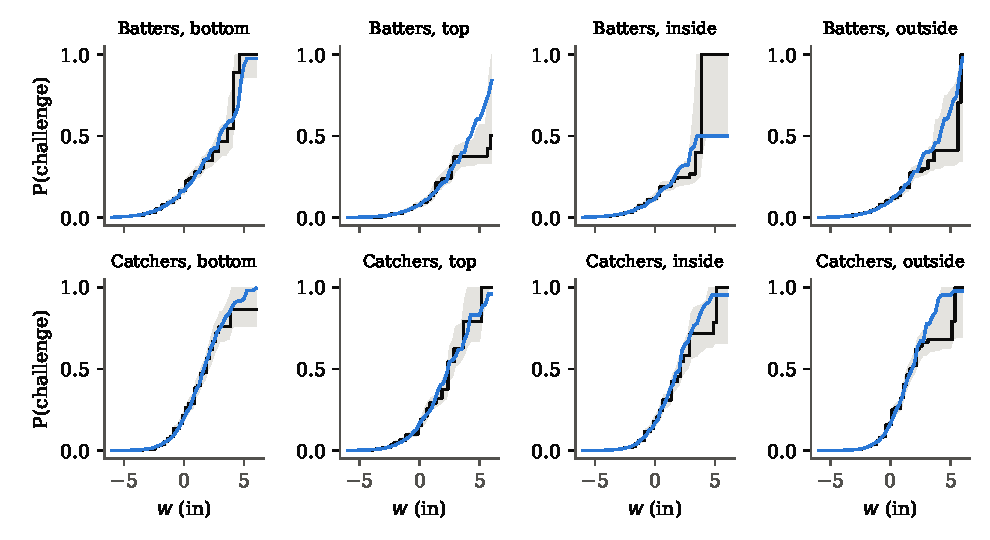
\includegraphics[width=\textwidth]{figures/fig_isotonic}
\caption{Challenge probability against the truth margin $w$ (inches, positive: the call was wrong), by side and zone
region. Black: isotonic regression of the observed challenges with pointwise 95\% game-bootstrap band (grey). Blue:
fitted comparator (probit), averaged over the same pitches.}\label{fig:isotonic}
\end{figure}

\paragraph{Player heterogeneity} Player random effects on $(\kappa,\log\sigma_r)$ improve the likelihood by
\DLLREvsMain{} points over the comparator, and with a lapse rate on top they have the best BIC (\BICRELapse). The
effects sit mostly in the criterion: the SD of the player criteria is \REKappaSDBatter\,in for batters and
\REKappaSDCatcher\,in for catchers, against an SD of $\log\sigma_r$ of \RELogSrSDBatter{} and \RELogSrSDCatcher. Both
random-effects fits are refined by Newton steps on a central-difference Hessian of the exact likelihood gradient after
L-BFGS, to a maximum gradient of $3\times10^{-8}$ with the lapse and $9\times10^{-4}$ without it (the earlier
quasi-Newton fits stopped at gradients of $0.1$--$1.3$). To evaluate policies each player's criterion and noise effects
are drawn \emph{jointly} from a bivariate normal with the posterior means and covariance computed on the quadrature
nodes (posterior correlation about 0.6 on average; a moment-matched approximation, not a draw from the node weights),
the belief is calibrated within the player's noise quintile, and the DP is solved with these posteriors. In the full
policy cross-fit the posteriors are those of each training fit, with $J=4$ joint draws per fold
(Section~\ref{sec:pcfdetail}). The primary estimate and its interval are in Section~\Mref{sec:eval} and
Section~\ref{sec:bootstrap}. Integrated over the fitted
population law the primary model predicts \RECalIntOff{} batter challenges and \RECalIntDef{} fielding-side
challenges against \RECalObsOff{} and \RECalObsDef{} observed, and with each player's posterior mean plugged in
\RECalPlugOff{} and \RECalPlugDef; the homogeneous comparator predicts \RECalMainOff{} and \RECalMainDef. The
batters' shortfall of about \RECalOffPct\% under the Gaussian law of the player effects (a fifth of the batters never
challenged) is a misfit of that law, which the primary model's policy values inherit.

\paragraph{A time-varying criterion} Adding second-half (July--September) shifts to the criterion's intercept and its
slope on $\log g$ and to $\log\sigma_r$, for each side, improves the comparator's BIC by \TimeDBICnum{} (\TimeDBICLapse{}
with a lapse rate as well); the fielding side's criterion falls and its noise drops in the second half, as the
out-of-sample comparison below shows. Its gap under the primary intervention is \GapTime{} (full policy cross-fit,
Table~\Mref{tab:variants}).

\subsection{Out of sample and other leagues}\label{sec:oos}
We fit the model to March--June (\SOOSTrainGames{} games) and to July--September (\SOOSTestGames{} games) separately.
Perception noise is \SOOSTrainSrBatter\,in for batters and \SOOSTrainSrCatcher\,in for catchers in the first half and
\SOOSTestSrBatter{} and \SOOSTestSrCatcher\,in in the second. Table~\ref{tab:oosfull} predicts the challenge counts and
overturn rates of the second half from the first-half fit. Overturn rates transfer for both sides and batter challenge
counts nearly so, but catchers challenged \OOSCatcherExcess\% more than predicted, and their fitted decision noise
fell: the fielding side's decisions changed during the season. Wins lost under the comparator and the score-aware DP,
each half against its own benchmark, are \SOOSLostTrainTrain{} in the first half, \SOOSLostTestTrain{} in the second
half with the first-half model and \SOOSLostTestTest{} with the second-half model.

For Triple-A 2025 and spring training 2026 we use the Stats API feeds, projected to the plate's midpoint
(Table~\ref{tab:feeds}). The refitted perception noise is \AAASrBatter\,in \SAAASrBatterCI{} for batters and
\AAASrCatcher\,in \SAAASrCatcherCI{} for catchers in Triple-A, and \SpringSrBatter\,in \SSpringSrBatterCI{} and
\SpringSrCatcher\,in \SSpringSrCatcherCI{} in spring training (95\% intervals). Transported MLB parameters predict the
overturn rates there well but overpredict catcher challenges, again a criterion effect.

\begin{table}[!htbp]
\caption{Observed against predicted challenges and overturn rates (observed / predicted). ``Fit'': the sample the
parameters are estimated on.}\label{tab:oosfull}
\centering\small
\resizebox{\textwidth}{!}{\begin{tabular}{lcccc}
\toprule
& \multicolumn{2}{c}{Batter} & \multicolumn{2}{c}{Catcher} \\
Sample and parameters & Challenges & Overturn (\%) & Challenges & Overturn (\%) \\
\midrule
Mar--Jun, in sample & 2{,}488 / 2{,}484 & 47.7 / 49.0 & 2{,}835 / 2{,}828 & 58.2 / 58.8 \\
Jul--Sep, Mar--Jun fit & 2{,}271 / 2{,}188 & 50.2 / 50.4 & 2{,}949 / 2{,}418 & 57.7 / 58.3 \\
Jul--Sep, Jul--Sep fit & 2{,}271 / 2{,}269 & 50.2 / 51.0 & 2{,}949 / 2{,}941 & 57.7 / 57.8 \\
Triple-A 2025, MLB fit & 4{,}507 / 4{,}432 & 45.0 / 50.1 & 4{,}832 / 5{,}446 & 53.8 / 58.6 \\
Triple-A 2025, refit & 4{,}507 / 4{,}498 & 45.0 / 46.3 & 4{,}832 / 4{,}817 & 53.8 / 54.6 \\
Spring 2026, MLB fit & 886 / 915 & 45.7 / 52.8 & 1{,}019 / 1{,}225 & 59.5 / 63.1 \\
Spring 2026, refit & 886 / 881 & 45.7 / 46.3 & 1{,}019 / 1{,}007 & 59.5 / 57.5 \\
\bottomrule
\end{tabular}
}
\end{table}

\paragraph{Feed coordinates} Rebuilding the 2026 MLB data on the live feed's own coordinates, projected to the
midpoint, gives $\sigma_r$ of \FeedSrBatter{} and \FeedSrCatcher\,in in the baseline model and \SFeedMainSrBatter{}
and \SFeedMainSrCatcher\,in in the comparator, against \SrBaseBatter{} / \SrBaseCatcher{} and \SrBatter{} /
\SrCatcher\,in on Statcast; wins lost are \SFeedLost{} and \SFeedLostMain.

\paragraph{A frozen policy} The temporal cross-fit of the main text freezes every component estimated on March--June:
the WP engine, the stakes the player decides on and the run laws (from March--June Statcast); the perception fit,
refitted on those March--June stakes, so that no frozen component sees the full-season engine; the stake-tercile cut
points of the calibration cells; the belief maps (fitted on auxiliary draws of the March--June pitches); the
score-aware DP; and the constant~$\delta$. Applied to July--September, the value of a flip is scored at the
full-season stakes, the yardstick of the observed value; the truths and signals there are simulated from the frozen
model, so this checks that the fitted policy objects transfer over time, not observed out-of-sample welfare. Against the benchmark re-estimated on July--September on
the same draws, the frozen DP keeps \FrozenDPShare\% and the frozen rule \FrozenRuleShareRetro\%; with the full-season
engine instead of the March--June one the figures are \FrozenDPShareNoEng\% and \FrozenRuleShareRetroNoEng\% (wins lost
against the frozen DP \FrozenLostNoEng). If the July--September truths are drawn from the July--September fit instead,
the frozen DP keeps \FrozenDPShareWorldTest\% and teams lose \FrozenLostWorldTest{} against it.

\subsection{Identification and known-truth recovery}
Proposition~\Mref{prop:ident} is checked symbolically (Section~\ref{sec:kernel}, checks D1--D4). For the known-truth
experiment we simulate challenges and rulings from the fitted baseline model ($\sigma_r=\SRecovTruthBatter$ and
$\SRecovTruthCatcher$\,in, $\pi=\SRecovPiTruth\%$) on the real 2026 opportunities, refit from a start with $\sigma_r$
multiplied by 1.5, and repeat. Table~\ref{tab:recovery} reports the results. For the primary model
(\texttt{src/recovery\_primary.py}) we simulate \RecPN{} seasons from its fit, every player at his posterior mean, and
refit it from its estimate: the lapse rates come back with bias \RecPLapseBatter{} and \RecPLapseCatcher{} percentage
points (SD \RecPLapseSDBatter{} and \RecPLapseSDCatcher), $\sigma_r$ with \RecPSrBatter\% and \RecPSrCatcher\%, and the
SD of the batters' criterion effects \RecPSdKBatter\% low, as the shrunken generating effects predict. In this baseline experiment, under correct specification, the bias in $\sigma_r$ is a fraction of a percent. Tracking noise of 0.3\,in barely moves $\sigma_r$, in line with
Proposition~\Mref{prop:ident}(c), but it raises the fitted mislabel rate, which absorbs the induced disagreements near
the boundary. Heavy tails fitted as Gaussian bias $\sigma_r$ up by about a quarter, but among the laws we fitted the likelihood
prefers the Gaussian (Table~\ref{tab:allvariants}). Ignoring player heterogeneity (simulated with the SDs of an earlier
player-effects fit without lapses, \SREUsedBatter\,in in $\kappa$ and \SREUsedLogBatter{} in $\log\sigma_r$ for batters) also biases $\sigma_r$ up, which lowers the estimated value of
challenging. On the data the bias is smaller: the comparator's batter $\sigma_r$ is \HetDataBiasBatter\% above the
random-effects model's. The direct comparison is the accounting index: \Gap{} under the primary model against
\GapMain{} under the homogeneous comparator (full policy cross-fit).

\begin{table}[!htbp]
\caption{Known-truth recovery of perception noise on the real 2026 opportunities.}\label{tab:recovery}
\centering\small
\resizebox{\textwidth}{!}{\begin{tabular}{lcrrrrr}
\toprule
Data-generating process & Converged & \multicolumn{2}{c}{Bias of $\hat\sigma_r$ (\%)} & \multicolumn{2}{c}{SD of $\hat\sigma_r$ (in)} & Mean $\hat\pi$ (\%) \\
& & batter & catcher & batter & catcher & \\
\midrule
Correctly specified & 19/20 & $+0.3$ & $+0.1$ & 0.03 & 0.02 & 0.04 \\
0.3\,in tracking noise & 10/10 & $+0.7$ & $+1.3$ & 0.04 & 0.03 & 6.18 \\
$t_5$ perception noise & 10/10 & $+25.4$ & $+22.9$ & 0.07 & 0.02 & 0.04 \\
Player random effects & 10/10 & $+12.8$ & $+4.1$ & 0.04 & 0.02 & 0.06 \\
\bottomrule
\end{tabular}
}
\end{table}

\subsection{Wins lost against perception noise}\label{sec:breakeven}
The value of every policy falls as perception gets worse, the benchmark's fastest. Figure~\ref{fig:breakeven} and
Table~\ref{tab:breakeven} re-solve and re-evaluate the model with $\sigma_r$ multiplied by a common factor on both
sides, holding realised play fixed at \SObservedWins{} wins per team-season. Wins lost fall to $0.25$ when $\sigma_r$
is \BreakEvenPct\% larger than estimated (by linear interpolation) and to
zero near a factor of 1.3. The right panel is the profile log-likelihood of each side's $\sigma_r$ in the baseline model
on the same axis: at the break-even it is \BreakEvenLLBatter{} points below its maximum for batters and
\BreakEvenLLCatcher{} for catchers, and a $10\%$ error already costs \ProfileTenBatter{} and \ProfileTenCatcher.

\begin{figure}[!htbp]
\centering
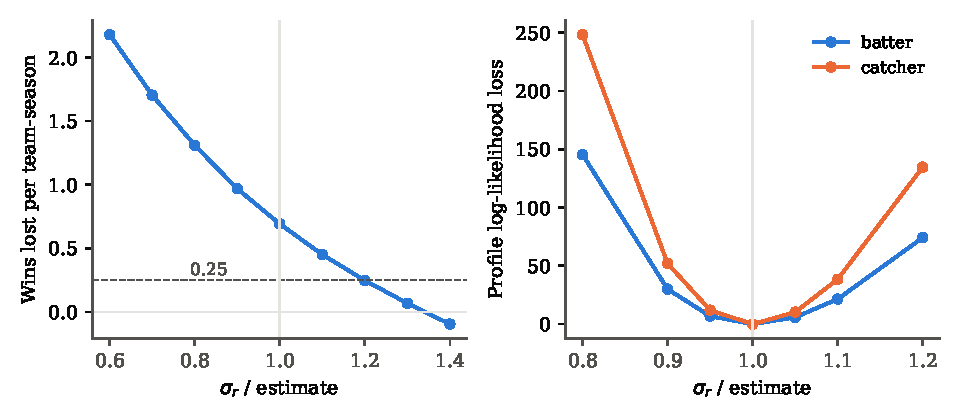
\includegraphics[width=.95\textwidth]{figures/fig_sr_breakeven}
\caption{Left: wins lost per team-season (score-aware benchmark minus realised play) when perception noise is a multiple
of its estimate; dashed line at $0.25$. Right: profile log-likelihood loss of $\sigma_r$ for each side, baseline
model.}\label{fig:breakeven}
\end{figure}

\begin{table}[!htbp]
\caption{Benchmark and wins lost per team-season when $\sigma_r$ is a multiple of its estimate, and the profile
log-likelihood loss at the multiples on the profile grid.}\label{tab:breakeven}
\centering\small
\begin{tabular}{rrrrrr}
\toprule
$\sigma_r$ / estimate & Benchmark & \multicolumn{2}{c}{Wins lost} & \multicolumn{2}{c}{Profile $-\Delta\ell$ (baseline model)} \\
& & score DP & pooled DP & batter & catcher \\
\midrule
0.6 & 5.52 & $+2.18$ & $+2.05$ & --- & --- \\
0.7 & 5.05 & $+1.70$ & $+1.58$ & --- & --- \\
0.8 & 4.66 & $+1.31$ & $+1.19$ & 145.4 & 248.2 \\
0.9 & 4.31 & $+0.97$ & $+0.86$ & 30.0 & 52.0 \\
1.0 & 4.04 & $+0.69$ & $+0.57$ & 0.0 & 0.0 \\
1.1 & 3.80 & $+0.45$ & $+0.33$ & 21.5 & 38.4 \\
1.2 & 3.59 & $+0.25$ & $+0.12$ & 74.2 & 134.7 \\
1.3 & 3.41 & $+0.07$ & $-0.04$ & --- & --- \\
1.4 & 3.25 & $-0.10$ & $-0.21$ & --- & --- \\
\bottomrule
\end{tabular}

\end{table}

\paragraph{Belief maps} Under the calibrated posterior the challenge threshold implied by the fitted criterion is on
average $p=\SThrCalBatter$ for batters and $\SThrCalCatcher$ for catchers; under a flat-prior belief map it would be
\SThrFlatBatter{} and \SThrFlatCatcher. Neither map makes the implied thresholds respond to leverage as the
cutoff~(\Mref{eq:bellman}) requires (Section~\Mref{sec:mech}).

%% ============================================================================================================
\section{Policy evaluation}\label{sec:policy}

\subsection{Simulated worlds}
Each simulated world keeps every real 2026 called pitch, its stake $g$, its known truth $W$ and the real call stream.
It draws the ruling with mislabel rate $\pi$, the signal $s=w+\varepsilon$ from the fitted perception model, and the
posterior $p=\Prob(Y=1\mid s)$ that the ruling overturns the call from a weighted isotonic regression of simulated truth on the signal
\citep{BarlowEtAl1972}. Under Gaussian noise the posterior is monotone in the signal; under Student-$t$ noise it need
not be (with prior mass $\tfrac12$ at $w=\pm1$ and $t_3$ noise it is $\tfrac12$, $\tfrac9{10}$ and $\tfrac{961}{1402}$
at signals 0, 2 and 10, tending to $\tfrac12$; \texttt{wolfram/rules\_scope.wl}), so for the $t$ rows the isotonic
map is a monotone approximation to their posterior, not the posterior itself. The isotonic map is fitted on an auxiliary, independent draw, so that the truth that scores a
policy never enters its decision. Fitting it on the scoring draw instead changed the benchmark by \SCrossFitOpt{} and the
one-line rule by \SCrossFitRule{} wins per team-season (average over $R=\SCrossFitR$ draws). Every policy runs on the
same draws, holding the challenges it would hold, with the extra-inning grant of Section~\ref{sec:counters}.
Table~\ref{tab:roles} splits the value of every policy by side.

\begin{table}[!htbp]
\caption{Wins per team-season by side and challenges per team-game (95\% game-bootstrap interval); the comparator with
the stakes cross-fitted only (Table~\ref{tab:oldpolicies}).}\label{tab:roles}
\centering\small
\begin{tabular}{lrrc}
\toprule
Policy & Wins, batters & Wins, fielding side & Challenges per team-game \\
\midrule
Optimum (score-aware DP) & 1.83 & 2.20 & 2.71 [2.67, 2.75] \\
Runs-objective rule & 1.78 & 2.17 & 2.98 [2.94, 3.02] \\
Pooled DP & 1.78 & 2.14 & 2.68 [2.65, 2.73] \\
One-line rule, $\delta=0.008$ & 1.73 & 2.12 & 2.21 [2.15, 2.27] \\
One-line rule, $\delta=0.01$ & 1.67 & 2.10 & 1.90 [1.84, 1.96] \\
48-cell card, published & 1.69 & 2.11 & 2.59 [2.54, 2.64] \\
48-cell card, refit & 1.67 & 2.09 & 2.52 [2.47, 2.56] \\
Observed 2026 (realised) & 1.44 & 1.90 & 2.17 [2.13, 2.22] \\
Fitted behavioural rule & 1.43 & 1.88 & 2.15 [2.12, 2.19] \\
Fixed 0.2-run rule & 0.96 & 1.51 & 1.02 [0.99, 1.08] \\
\bottomrule
\end{tabular}

\end{table}

\subsection{Competitor rules}
\emph{Runs-objective rule} \citep{Namuduri2026runs}: challenge iff $p\,\mathrm{RV}>(1-p)C(t,c)$, where RV is the run
value of the flip and $C$ the run value of a challenge at the start of the half-inning, from the same DP solved with
runs as the objective. His code indexes $C$ by incorrect challenges spent, which maps to our $c$.
\emph{48-cell card} \citep{Arora2026use}: a threshold on $p$ for each inning band (1--3, 4--6, 7--8, 9+), tercile of
$g$ over all opportunities, count class (PA-ending iff three balls or two strikes) and challenges held. ``Published''
uses his 2026 thresholds with our terciles of $g$; ``refit'' fills each cell with the median break-even $D/(g+D)$ of our
DP over the opportunities in it, a reproduction of his fitting procedure on our model; a card whose cells were
chosen to maximise value could do better. Our tercile medians of $g$ are close to his.
\emph{Savant's form, tuned}: $p\ge c/(c+\mathrm{RV})$ with $c$ on a grid of run costs, the best chosen at the point
estimate (\SavantTunedC{} runs).
\emph{Fixed 0.2-run rule} \citep{Savant2026abs,Tango2026costbenefit}: challenge iff $p\ge0.2/(0.2+\mathrm{RV})$. The
league computes RV from an RE288 run-expectancy table; we compute it from our own run-expectancy engine, whose run
swings are slightly smaller on average, so our version of the rule is marginally more conservative. The ranking does
not depend on this: an independent recomputation on Statcast's own run- and win-expectancy changes gives
\SIndSavant{} wins per team-season for the rule against \SIndObs{} for observed play (ratio \SIndSavantRatio) and
\SIndRule{} for the one-line rule. All competitors and the one-line rule are cutoff rules in $p$
(Section~\ref{sec:kernel}).

\begin{table}[!htbp]
\caption{The earlier estimator: the comparator with the stakes cross-fitted only (decision model, beliefs and DP fitted
on all games), wins per team-season with 95\% joint-bootstrap percentile intervals ($B=\JointBootB$); top, the benchmark
and observed play; bottom, every public rule rebuilt on our model, with the share of the benchmark and of the gap it
recovers.}\label{tab:oldpolicies}
\centering\small
\begin{tabular}{p{5.0cm}ccc}
\toprule
Policy & Wins & Share of benchmark (\%) & Challenges \\
\midrule
Pooled-model benchmark (primary intervention) & 3.99 [3.81, 4.16] & 100 & 2.70 \\
Earlier DP (no score, fixed opportunity counts) & 3.88 [3.70, 4.04] & 97.2 [96.4, 98.0] & 2.68 \\
Clairvoyant comparator (knows its game's future $(p,g)$; not a bound) & 4.80 [4.59, 5.00] & 120.2 [118.5, 121.9] & 3.41 \\
Teams' fitted rule $s>\kappa(x)$ (simulated) & 3.31 [3.14, 3.44] & 82.9 [81.1, 84.6] & 2.16 \\
\textbf{Observed 2026 (realised)} & 3.34 [3.16, 3.52] & 83.7 [81.0, 86.8] & 2.18 \\
\bottomrule
\end{tabular}


\medskip
\begin{tabular}{p{4.6cm}ccc}
\toprule
Rule & Share of benchmark (\%) & Gap recovered (\%) & Challenges \\
\midrule
Runs-objective rule \citep{Namuduri2026runs} & 98.1 [97.3, 98.7] & 88 & 2.98 \\
One-line rule, $\delta=0.008$ & 95.4 [94.2, 96.0] & 72 & 2.22 \\
One-line rule, $\delta=0.01$ & 93.0 [91.9, 94.1] & 57 & 1.90 \\
48-cell card, median DP thresholds & 93.2 [92.2, 94.5] & 58 & 2.51 \\
48-cell card, published \citep{Arora2026use} & 94.3 [93.3, 95.6] & 65 & 2.59 \\
Fixed 0.2-run rule \citep{Savant2026abs} & 61.4 [59.1, 64.2] & \ensuremath{-}137 & 1.03 \\
Savant's form, run cost 0.08 & 92.1 [90.8, 93.1] & 52 & 2.44 \\
One-line rule at the teams' challenge rate & --- & 68 [61, 75] & 2.18 \\
\bottomrule
\end{tabular}

\end{table}

\subsection{Causal re-simulation}\label{sec:causal}
The path-sum value of a policy is the sum of $g$ over its successful challenges, each $g$ read off the recorded game.
After the first flip the recorded continuation is no longer the game that would have been played. For each team-game and policy we find the first divergence between the policy's game and the recorded
game: the first called pitch whose call exactly one of them flips (\SBranches{} branch points per team-game for the
benchmark, \CausalSkipShare\% of them recorded overturns the policy would have skipped). Before it the two games
coincide, so the path sum is exact up to there. At that pitch three worlds are simulated with common random numbers:
\begin{itemize}
\item[A:] the call is flipped and the game continues, the team following the policy with the challenges it holds;
\item[A$'$:] the original call stands and the team keeps following the policy;
\item[B:] the original call stands and the team never challenges again.
\end{itemize}
In all three the opponent follows its fitted behavioural rule $s>\kappa(x)$ with its recorded remaining challenges.
If the policy flips a call the team left standing, A is the policy's world and A$'$ the recorded one; if the team
flipped a call the policy leaves standing, A (the flipped call) is the recorded world and A$'$ the policy's, and every
correction below enters with the opposite sign.
Up to the branch pitch the policy's game and the recorded game coincide, so their values agree up to it; this is the
anchor. For a branch at which the policy flips a call the team left standing, the path-sum value of the team-game from
the branch on is $g_{\rm branch}+L_{\rm rec}$, with $L_{\rm rec}$ the team's later gains on the recorded continuation,
and the causal value is $g_{\rm branch}+\E[L\mid\text{flip}]$. For a branch at which the team flipped a call the policy
leaves standing, the path sum omits $g_{\rm branch}$ and still uses the recorded (flip) continuation for the policy, so
the roles of A and A$'$ swap and the correction changes sign; the inventories in the two worlds then differ by the
challenge the team kept. Two estimators of the correction:
\begin{align*}
\text{RB:}\quad & \text{causal}=\text{path}+\E[(L_A-O_A)-(L_{A'}-O_{A'})], \\
\text{win count:}\quad & \text{causal}=\text{path}+\E[\text{win}_A-\text{win}_{A'}]-g_{\rm branch},
\end{align*}
where $L$ ($O$) sums $g$ over the team's (the opponent's) later successful flips at the simulated state. If the WP
engine is the simulator's value function, the team's win indicator is a martingale whose jump at each later flip is
$+g$ for the team's flips and $-g$ for the opponent's, so
$\E[\text{win}_A-\text{win}_{A'}]=g_{\rm branch}+\E[(L_A-O_A)-(L_{A'}-O_{A'})]$ and the two estimators agree. The
opponent term matters because the flip changes the opponent's later opportunities too; dropping it (the team's own
gains only) changes the benchmark's RB value by \SCausalOppEffect{} wins per team-season; RB is the low-variance
version (the decomposition is checked in Section~\ref{sec:kernel}). Differencing against A$'$ cancels any level bias of
the simulator's opportunity stream.

\paragraph{The complete contrast} Both A and A$'$ follow the policy after the branch, so the corrections above replace
only the first divergence; later divergences between the policy and the recorded game are still valued on the
recorded path. A small example shows the consequence. With one retained challenge that always succeeds, a recorded
team that never challenges, and three opportunities worth $0.1$, $0.2$ (which ends the opportunities when taken) and
$0.1$, a policy that always challenges gains $0.3$, the path sum credits $0.4$ and the first-divergence correction
also gives $0.4$. The complete contrast simulates, from the first divergence, world P (the policy's call, then the
policy) against world B (the team's call, then its fitted behavioural rule $s>\kappa(x)$ at the simulated state, with
the challenges the team held), with the opponent's fitted rule in both and common random numbers. Before the branch the
two games coincide, so the gain of the policy over the behavioural rule in a team-game is $\E[\text{win}_P-\text{win}_B]$,
or, valued by later stakes, $\E[(g_{\rm b}\mathbf 1_P+L_P-O_P)-(g_{\rm b}\mathbf 1_B+L_B-O_B)]$ with $\mathbf 1_P$
($\mathbf 1_B$) indicating that the policy (the team) flipped the branch call. This contrast starts from the
\emph{recorded} game (the first divergence is against the recorded challenges, and the team holds its recorded
inventory) and continues the team with its fitted rule, so its path-sum counterpart is the path sum against the
observed challenges: for the benchmark it gives \FullRB{} \FullRBCI{} (value) and \FullWin{} \FullWinCI{} (win count)
wins per team-season, against \FullPathObs{} for the path sum minus the observed value.

\paragraph{The paired contrast} To compare two simulated policies like with like, the teams' fitted behavioural rule
is played along the stream in the same world as the policy (same truths and signals), with its own inventory, and the
policy is branched against \emph{it} at the first pitch where their flips differ (\texttt{policies.path\_trace}). From
there world P (the policy's call, then the policy, holding its simulated count) and world B (the rule's call, then the
rule, holding the rule's simulated count) are simulated to the end of the game, the opponent following its rule from
its own simulated count in both. Its path-sum counterpart is the path sum of the policy minus that of the simulated
rule on the same worlds. For the benchmark: \PairRB{} \PairRBCI{} valued by later stakes, \PairWin{} counting wins,
against \PairPath{} by the path sum. The win-count and the stake-valued estimators differ by about \WinMinusRBAbs{} in
both contrasts; part of that is the simulator's flip swing, which falls \SimGShareRunGap\% short of $g$
(Section~\ref{sec:causalgap}), and part we cannot attribute. The behavioural rule against itself gives zero.

\paragraph{Simulator} Pitch events (called pitch, swinging strike or foul tip, foul, ball in play, hit by pitch,
automatic ball) by count, outs and bases from 2026 Statcast; called pitches drawn from the 2026 called-pitch pool of
the same count, each with its location, truth and signal; in-play
outcomes (outs, bases and runs) by count, outs and bases; for a drawn called pitch the criterion and the belief are
recomputed at the simulated inning, stake and challenges held (a pool row keeps only its location, truth and signal);
the DP's state uses the same encoding as the DP, including extra innings; baserunning between pitches (steals, wild pitches, passed
balls and pickoffs, on about \SGapMoveRate\% of pitches); the runner on second in extra innings; the extra-inning
challenge grant; walk-off rules. We use $K=\CausalK$ play-outs per world and $R=\CausalR$ independent draws of the
perception signals.

\paragraph{Checks} In world B the simulator's win rate minus the WP engine's is between \SCalibWinBLo{} and
\SCalibWinBHi{} across policies, with calibration slope \SCalibSlope. The offset is the team giving up its challenges
while the opponent keeps its own, and it is the same at home and away. Its no-flip continuation produces about the
same later value as the recorded games (\SLaterNoflip{} against \SLaterRecorded{} wins per team-season for the
benchmark; difference \SFidelity{} \SFidelityCI), and the A$-$A$'$ difference cancels any level gap.

\begin{table}[!htbp]
\caption{Path-sum and causal values, wins per team-season, with 95\% intervals for the differences from
\CausalBootN{} game resamples of the per-game outputs at fixed fitted parameters.}\label{tab:causal}
\centering\scriptsize
\resizebox{\textwidth}{!}{\begin{tabular}{lrrrcc}
\toprule
Policy & Path sum & RB & Win count & RB $-$ path & Win count $-$ RB \\
\midrule
Optimum (score-aware DP) & 4.04 & 4.04 & 4.01 & $+0.000$ [\ensuremath{-}0.001, 0.002] & $-0.03$ [\ensuremath{-}0.05, \ensuremath{-}0.01] \\
Runs-objective rule & 3.95 & 3.95 & 3.93 & $+0.002$ [0.000, 0.003] & $-0.02$ [\ensuremath{-}0.04, 0.00] \\
Pooled DP & 3.93 & 3.93 & 3.91 & $+0.004$ [0.002, 0.005] & $-0.02$ [\ensuremath{-}0.04, \ensuremath{-}0.01] \\
One-line rule, $\delta=0.008$ & 3.86 & 3.86 & 3.83 & $+0.001$ [\ensuremath{-}0.001, 0.002] & $-0.02$ [\ensuremath{-}0.04, \ensuremath{-}0.01] \\
One-line rule, $\delta=0.01$ & 3.76 & 3.76 & 3.74 & $+0.001$ [\ensuremath{-}0.001, 0.003] & $-0.02$ [\ensuremath{-}0.04, \ensuremath{-}0.01] \\
48-cell card, published & 3.82 & 3.82 & 3.82 & $+0.002$ [0.000, 0.004] & $-0.00$ [\ensuremath{-}0.02, 0.01] \\
48-cell card, refit & 3.78 & 3.78 & 3.76 & $+0.001$ [\ensuremath{-}0.001, 0.003] & $-0.02$ [\ensuremath{-}0.04, 0.00] \\
Fitted behavioural rule & 3.31 & 3.31 & 3.30 & $+0.001$ [0.000, 0.003] & $-0.01$ [\ensuremath{-}0.02, 0.01] \\
Fixed 0.2-run rule & 2.47 & 2.47 & 2.46 & $+0.001$ [0.000, 0.003] & $-0.01$ [\ensuremath{-}0.03, 0.01] \\
\bottomrule
\end{tabular}
}
\end{table}

\paragraph{Results} Table~\ref{tab:causal}: the RB causal value is within a few thousandths of a win of the path sum
for every policy. The win-count estimator differs by \BinaryMinusRB{} \BinaryMinusRBCI{} wins for the benchmark, which
puts the wins lost at \BinaryLost{} \BinaryLostCI{} on that measure; averaged over the \SGapNPolicies{} policies the
difference is \SGapAvgNew. Section~\ref{sec:causalgap} explains the remaining difference.

\subsection{Simulator against WP engine}\label{sec:causalgap}
The two estimators agree exactly when the simulator's value function is the WP engine. They differ, to first order,
by the sum over branch flips of the difference between the simulator's swing in win probability and the engine's $g$.
To measure that difference without Monte Carlo error we write each simulator as an exact pitch-level Markov chain and
compute its win probabilities and its $g$ at every branch flip of the benchmark (\SGapBranches{} per team-season, mean
engine $g$ \SGapMeanG). The simulator itself reproduces its chain: from 400 branch states and 2,000 play-outs each,
the simulated flip swing minus the chain's is \SGapMCNew{} (SE \SGapMCNewSE), and the simulated home win rate minus
the engine's is \SGapLevelNew.

Table~\ref{tab:gap} adds the simulator's ingredients one at a time. A simulator whose in-play outcomes ignore the
count and that has no baserunning between pitches moves win probability by only \SimGShare\% of $g$. That shortfall
predicts a win-count minus RB difference of $\GapPredSim$ wins per team-season for the benchmark; the difference
measured with that simulator is \SGapMeasOld{} \SGapMeasOldCI, the same sign but smaller. (In the headline run, the
simpler simulator's win-count estimate fell short of the $g$-based accounting by \BinaryMinusRBSimAbs{} wins.) Batters ahead in the count do more damage on contact, so a count-blind in-play distribution compresses the
value of turning a strike into a ball, and the extra pitches a ball buys also give runners more chances to advance.
With both ingredients the simulator reaches \SimGShareRun\% of $g$; the predicted difference is $\GapPredRun$, while the
one measured in this decomposition run is \SGapMeasNew{} \SGapMeasNewCI{} (\BinaryMinusRB{} in the headline run). The
shortfall in $g$ therefore explains the sign of the difference but not all of its size; the rest is a difference in
win probability between the simulator and the engine that the first-order expansion does not capture, such as the
simulator's level offset (world B) at the branch states. Table~\ref{tab:gapcount} shows that the shortfall of the simpler
simulator was largest for flips early in the count.

The path sum is priced in engine $g$, and the engine is the object calibrated to real outcomes: its distribution of
plate-appearance outcomes is the empirical one from every 2026 pitch, and it predicts game outcomes as well as
Statcast's own win expectancy (Section~\ref{sec:bootstrap}). A residual mismatch between simulator and engine biases
the win-count estimate but not the path sum or the RB estimate, which is why the headline uses the path sum.

\emph{Home field.} Neither the engine nor the simulator has a home-field term, so it cannot separate them. Estimating
the engine with separate plate-appearance distributions for home and away batters gives the home team a win
probability of \SGapHomeWP{} at the first pitch, changes $g$ at the benchmark's branch flips by about $-\HomeFieldRelG\%$
and changes the wins lost by $\HomeFieldLostChange$.

\begin{table}[!htbp]
\caption{Simulator against WP engine at the benchmark's branch flips: the simulator's swing in win probability as a share
of the engine's $g$ (exact chain), and the win-count minus RB difference that the mismatch predicts, wins per
team-season. Each row adds one ingredient to the row above.}\label{tab:gap}
\centering\small
\resizebox{\textwidth}{!}{\begin{tabular}{p{7.5cm}rr}
\toprule
Simulator & $g$ / engine $g$ (\%) & Predicted win count $-$ RB \\
\midrule
Events by count; in-play outcome by the plate appearance's starting outs and bases & 95.4 & $-0.079$ \\
+ in-play outcome by count, outs and bases & --- & $-0.044$ \\
+ pitch events by outs and bases & --- & $-0.064$ \\
+ baserunning between pitches (simulator used) & 98.8 & $-0.010$ \\
WP engine & 100 & $0$ \\
\bottomrule
\end{tabular}
}
\end{table}

\begin{table}[!htbp]
\caption{Simulator swing relative to engine $g$, minus one, by the count of the branch pitch (benchmark).}\label{tab:gapcount}
\centering\scriptsize
\begin{tabular}{lrrrrr}
\toprule
Count & $n$ & \multicolumn{4}{c}{$g$ / engine $g$ $-1$ (\%)} \\
 & & first simulator & + contact by count & + events by outs, bases & + baserunning \\
\midrule
0-0 & 3{,}005 & $-11.0$ & $+1.6$ & $-0.4$ & $+1.3$ \\
0-1 & 1{,}027 & $-8.6$ & $-0.2$ & $-0.5$ & $+1.3$ \\
0-2 & 617 & $-1.2$ & $-4.9$ & $-4.7$ & $-2.2$ \\
1-0 & 1{,}414 & $-9.8$ & $-3.4$ & $-6.5$ & $-4.5$ \\
1-1 & 1{,}027 & $-8.3$ & $+0.3$ & $-0.4$ & $+1.2$ \\
1-2 & 965 & $-1.9$ & $-2.9$ & $-3.3$ & $-0.9$ \\
2-0 & 740 & $+4.5$ & $+3.1$ & $-0.7$ & $+2.2$ \\
2-1 & 783 & $-4.5$ & $-1.5$ & $-1.8$ & $+0.7$ \\
2-2 & 1{,}105 & $-2.5$ & $-3.6$ & $-3.8$ & $-1.2$ \\
3-0 & 337 & $-1.7$ & $-6.7$ & $-6.8$ & $-3.2$ \\
3-1 & 547 & $-0.9$ & $-2.8$ & $-3.3$ & $+0.2$ \\
3-2 & 1{,}024 & $-1.2$ & $-2.8$ & $-3.4$ & $-0.4$ \\
\bottomrule
\end{tabular}

\end{table}

\subsection{Behavioural rule against realised play}\label{sec:behaviourgap}
The fitted behavioural rule $s>\kappa(x)$ of the comparator, simulated holding the challenges it would hold, earns
\WFitRule{} \WFitRuleCI{} wins per team-season against \WObs{} realised. Table~\ref{tab:behaviourgap} compares the two
by stake quintile, with the model's expectation taken pitch by pitch at the challenges actually held: the expected
value of the teams' challenges is \BGValueExpected{} wins per team-season against \BGValueObserved{} realised, and in
the top fifth of stakes the teams made \BGTopChExcess{} more challenges than the model expects and gained
\BGTopValueExcess{} more wins.

With a criterion linear in $\log g$, the previous comparator, the simulated rule earned \KGFitRuleMain{} wins and the
excess in the top quintile was large: the real response to the stake is steeper at the top than a linear criterion
allows. The comparator's piecewise-linear criterion (hinges at $\log g=-5.0$, $-4.0$ and $-3.2$, about the 40th, 80th
and 95th percentiles) improves the log-likelihood by \KGDLL{} points with \KGK{} more parameters (BIC better by
\KGDBIC), raises the simulated rule to \KGFitRule{} and leaves the decision noise practically unchanged
(\KGSrBatter\,in for batters and \KGSrCatcher\,in for catchers, against the linear model's values), so the benchmark
hardly moves (\KGOpt{} against \KGOptMain{} wins on the same $R=\KGR$ draws). The comparison of the benchmark with realised
play uses the behavioural model only through the decision noise it reveals.

\begin{table}[!htbp]
\caption{Observed against model-expected challenges, overturns and value by stake quintile (comparator, expectation at
the challenges actually held). Value: sum of $g$ over overturned challenges, wins per team-season.}\label{tab:behaviourgap}
\centering\small
\resizebox{\textwidth}{!}{\begin{tabular}{llrrrrrr}
\toprule
Side & Stake quintile & Mean $g$ & \multicolumn{2}{c}{Challenges} & \multicolumn{2}{c}{Overturned} & Value obs.\ $-$ exp. \\
 & & & obs. & exp. & obs. & exp. & (wins/team-season) \\
\midrule
Batters & 1 & 0.0015 & 827 & 820 & 416 & 440 & $-0.000$ \\
 & 2 & 0.0050 & 579 & 618 & 312 & 338 & $-0.005$ \\
 & 3 & 0.0080 & 597 & 599 & 316 & 332 & $-0.005$ \\
 & 4 & 0.0130 & 996 & 953 & 527 & 497 & $+0.012$ \\
 & 5 & 0.0335 & 1{,}760 & 1{,}763 & 756 & 765 & $-0.012$ \\
\addlinespace
Fielding side & 1 & 0.0015 & 1{,}009 & 1{,}022 & 551 & 590 & $-0.001$ \\
 & 2 & 0.0050 & 921 & 874 & 587 & 570 & $+0.003$ \\
 & 3 & 0.0081 & 861 & 878 & 558 & 568 & $-0.003$ \\
 & 4 & 0.0131 & 1{,}092 & 1{,}125 & 672 & 668 & $+0.003$ \\
 & 5 & 0.0360 & 1{,}901 & 1{,}868 & 984 & 965 & $+0.030$ \\
\bottomrule
\end{tabular}
}
\end{table}

\subsection{Thresholds by stake}\label{sec:mechanism}
Table~\ref{tab:mechanism} gives, by stake quintile, the confidence threshold the teams' fitted criterion implies
through the calibrated belief map and the DP benchmark's threshold $D/(g+D)$ at the recorded state, and the same in
inches of signal: the teams' criterion $\kappa$ and the signal at which the belief reaches the one-line rule's
threshold $\RuleDelta/(g+\RuleDelta)$. Teams' thresholds fall far less with the stake than the benchmark's.

\begin{table}[!htbp]
\caption{Revealed and benchmark thresholds by stake quintile (eligible pitches, comparator, $R$ draws of the belief
map). Signal thresholds are averages over the pitches of the quintile.}\label{tab:mechanism}
\centering\small
\begin{tabular}{llrrrrr}
\toprule
Side & Stake quintile & Median $g$ & \multicolumn{2}{c}{Confidence threshold $p^\ast$} & \multicolumn{2}{c}{Signal threshold (in)} \\
 & & & teams & DP benchmark & teams $\kappa$ & one-line rule \\
\midrule
Batters & 1 & 0.0014 & 0.46 & 0.65 & 4.1 & 9.3 \\
 & 2 & 0.0052 & 0.48 & 0.55 & 4.5 & 6.7 \\
 & 3 & 0.0081 & 0.47 & 0.48 & 4.5 & 5.1 \\
 & 4 & 0.0136 & 0.44 & 0.34 & 3.7 & 3.0 \\
 & 5 & 0.0281 & 0.35 & 0.19 & 2.4 & 0.3 \\
\addlinespace
Fielding side & 1 & 0.0013 & 0.45 & 0.65 & 1.8 & 4.9 \\
 & 2 & 0.0051 & 0.50 & 0.55 & 2.1 & 2.9 \\
 & 3 & 0.0082 & 0.50 & 0.47 & 2.1 & 2.1 \\
 & 4 & 0.0138 & 0.44 & 0.34 & 1.7 & 1.2 \\
 & 5 & 0.0300 & 0.35 & 0.19 & 1.1 & 0.0 \\
\bottomrule
\end{tabular}

\end{table}

\subsection{The flat-optimum bound on the calibrated pools}\label{sec:flat}
To evaluate Theorem~\ref{thm:flatS} exactly we need a model in which its assumptions hold. We use the score-aware
calibrated DP restricted to regulation: the exogenous state is the half-inning and the home score difference at its
start; the number of opportunities in a half-inning follows its empirical law in that state (as in the DP) and
their $(g,p)$ are drawn i.i.d.\ from the 2026 pool of that state; runs between half-innings come from their empirical law; and the game ends after the top of the ninth if the
home team leads and after the ninth otherwise. In this model the MDP is exact, so identity (i) must hold to rounding.
Bound (ii) needs the density bound $M$; we estimate it as the largest histogram density of $p$ (bin width $0.025$)
within quintiles of $g$, and the ``local'' approximation replaces it by the density at the midpoint of each interval.
Table~\ref{tab:flat} gives the results ($R=\SFlatR$ draws). Identity (i) holds to the printed precision; the best
constant $\delta=\FlatBestDelta$ loses \FlatLoss\%; the local approximation is close (\FlatLocal\%); and (ii) with
the histogram heights gives \FlatBound. Because the calibrated posterior is a step function of the signal (it is
fitted on bins of 0.1\,in), its law has atoms and no density, so that number is a smoothed approximation, not a
certified bound; identity (i) needs no density. On the real game stream the same rule loses \RuleLossStream\%. The two
problems differ: in the exact model the DP is optimal by construction, while on the real stream it is optimal for the
pooled law it was solved on, not for the realised sequence of calls and stakes, and the real stream includes extra
innings, where the top-up rule makes the DP and the rule act alike. The rule's share is relative to the benchmark,
and a richer-state policy could do better than the benchmark.

\begin{table}[!htbp]
\caption{Theorem~\ref{thm:flatS} on the calibrated pools, home and away sides pooled. Loss: $1-V^\delta/V^\star$.
Identity gap: largest difference between $V^\star-V^\delta$ and the sum in (i).}\label{tab:flat}
\centering\small
\begin{tabular}{rrrrrr}
\toprule
$\delta$ & $V^\delta/V^\star$ (\%) & Loss (\%) & Local approx.\ (\%) & Bound (ii) (\%) & Identity gap \\
\midrule
0.004 & 80.1 & 19.9 & 15.9 & 49.9 & $0$ \\
0.005 & 87.3 & 12.7 & 10.8 & 36.8 & $0$ \\
0.006 & 91.5 & 8.5 & 7.7 & 32.7 & $0$ \\
0.007 & 93.6 & 6.4 & 6.3 & 36.1 & $0$ \\
0.008 & 94.0 & 6.0 & 6.4 & 45.5 & $0$ \\
0.009 & 93.3 & 6.7 & 7.6 & 59.0 & $0$ \\
0.010 & 91.9 & 8.1 & 9.3 & 76.2 & $0$ \\
0.012 & 87.7 & 12.3 & 14.1 & 118.9 & $0$ \\
0.015 & 80.3 & 19.7 & 22.7 & 196.4 & $0$ \\
0.020 & 68.6 & 31.4 & 36.3 & 343.4 & $0$ \\
\bottomrule
\end{tabular}

\end{table}

\subsection{Stakes validation}\label{sec:stakesval}
\emph{Statcast's contrast.} Statcast's \texttt{home\_win\_exp} takes a single value in each of its observed pre-pitch
states (inning, half, outs, bases, score, count), so it is a table, and its ball-versus-strike contrast at a state is
the table's value after a ball minus its value after a strike: the next count's entry for $b<3$ and $s<2$, and for ball
four and strike three the median of $\texttt{home\_win\_exp}+\texttt{delta\_home\_win\_exp}$ over the walks and
strikeouts observed at that state. The contrast exists for \SVSharePct\% of the called pitches; the rest are states
whose after-state Statcast never visited. Its values are rounded to 0.001. Table~\ref{tab:svcells} compares it with
ours by decile of our stake; the correlation over all pitches is \SVCorr. Engines fitted on random halves of the games
give contrasts that correlate at \SVHalfCorr{} with each other.
\begin{table}[!htbp]
\caption{Ball-versus-strike contrast (batting team, WP): ours against Statcast's own win expectancy, by decile of our
stake $g$.}\label{tab:svcells}
\centering\small
\begin{tabular}{rrrrr}
\toprule
Leverage decile & Pitches & Mean $g$, ours & Mean $g$, Statcast & Correlation \\
\midrule
1 & 35{,}030 & 0.0006 & 0.0007 & 0.174 \\
2 & 35{,}097 & 0.0025 & 0.0026 & 0.400 \\
3 & 34{,}966 & 0.0043 & 0.0044 & 0.350 \\
4 & 35{,}013 & 0.0060 & 0.0062 & 0.229 \\
5 & 35{,}117 & 0.0075 & 0.0079 & 0.217 \\
6 & 34{,}954 & 0.0092 & 0.0095 & 0.306 \\
7 & 35{,}020 & 0.0118 & 0.0122 & 0.285 \\
8 & 35{,}019 & 0.0159 & 0.0159 & 0.398 \\
9 & 35{,}030 & 0.0227 & 0.0224 & 0.547 \\
10 & 35{,}014 & 0.0492 & 0.0485 & 0.963 \\
\bottomrule
\end{tabular}

\end{table}

\emph{Outcomes near the edge.} For called pitches within 2\,in of the ABS edge, in games not used to fit the engine,
we regress $Y-\mathrm{WP}_{\rm strike}$ on $(1,\mathrm{WP}_{\rm strike},\mathbf 1\{\text{ball}\}\,g)$ by least squares
with game-clustered errors, where $Y$ is the batting team's win and the call is the one that stood after any
challenge. Within that band the ABS call turns on fractions of an inch; we assume that given the state the call is then close to
randomised. Within the band the pre-pitch covariates are balanced between balls and strikes except the strike count
(standardised difference \EdgeStrikesSD; at most \EdgeOtherSDMax{} for outs, runners, inning, score, side, batter's
hand and $\log g$), the umpire's count-dependent zone; we have not checked pitcher, umpire or pitch characteristics. The
call is the one that stood after any challenge; with the umpire's original call instead the slope is \EdgeOrigSlope{}
\EdgeOrigSlopeCI. Under the assumption a correct contrast predicts a slope of one. Over five random splits the slope averages \SVSlope{} (SE about
\SVSlopeSE); the lower leverage terciles carry too little contrast to estimate a slope.

\emph{Other yardsticks.} On the pitches with a Statcast contrast (the others are dropped from the stream, so the
inventory runs over a shortened season rather than the full one), the whole analysis on Statcast's stakes (comparator refitted on all
games, DP re-solved, every policy re-simulated; neither cross-fitted nor out-of-fold) gives a gap of \SVLostSC; deciding on our full-season stakes and
scoring every flip at Statcast's contrast gives \SVLostOursSC, against \SVLostOursSame{} decided and scored on ours.
Every rule keeps its rank.

\emph{Where the cross-fitting effect comes from.} On two cross-fit splits, with common random numbers, the comparator
was evaluated with decisions on the full-season or the out-of-fold engine and scores at the full-season or the in-fold
engine (\texttt{crossfit.py decomp}). The gap is \XDFullFull{} deciding and scoring on the full-season engine,
\XDFullIn{} scoring the same decisions on the in-fold engine, \XDOutFull{} deciding on the out-of-fold engine and
scoring on the full-season one, and \XDOutIn{} cross-fitted: the drop appears only when decision and score use
independent engines. A single split's scoring engine adds noise of about $\pm0.02$ to the gap, which the average over
\XFitS{} splits removes.

\subsection{The intervention grid}\label{sec:pidfull}
For a perceptual share $\rho$ the simulated player sees $s_p=w+\sqrt\rho\,\sigma_r\varepsilon_1$; the belief map is
fitted on auxiliary draws of $s_p$, so the benchmark's belief is calibrated to the player's own signal; the teams'
behavioural rule decides on $s_p+\sqrt{1-\rho}\,\sigma_r\varepsilon_2$, so that its decision noise is the fitted
$\sigma_r$ for every $\rho$ (Proposition~\Mref{prop:ident}(d); in Mathematica, the convolution is exactly
$N(0,\sigma_r^2)$ and $\partial\Prob(\text{challenge}\mid w)/\partial\rho=0$, \texttt{wolfram/intervention.wl}). For a
removable lapse share $\ell$, the benchmark lapses on a pitch iff $u<(1-\ell)\lambda$, with the same uniform $u$ that
decides the behavioural rule's lapse ($u<\lambda$), and its DP is re-solved with the lapsed opportunities worth zero.
The grid of Table~\Mref{tab:pid} is part of the full policy cross-fit of the primary model and the comparator
($S=\GapS$ splits). Table~\ref{tab:pidall} gives the grid for every model at least as good as the comparator by BIC with
the stakes cross-fitted only, on one split ($R=\IVR$; Monte Carlo standard errors about 0.01).

\begin{table}[!htbp]
\caption{The accounting gap with the stakes cross-fitted only, one split, by model and intervention (the earlier
estimator; primary values of Table~\Mref{tab:pid} come from the full policy cross-fit).}\label{tab:pidall}
\centering\small
\begin{tabular}{lcccc}
\toprule
Model ($\ell$) & $\rho=1$ & $\rho=0.75$ & $\rho=0.5$ & $\rho=0.25$ \\
\midrule
Main & 0.65 & 1.06 & 1.64 & 2.71 \\
Main + lapse ($\ell=0$) & 0.48 & 0.81 & 1.34 & 2.27 \\
Main + lapse ($\ell=0.5$) & 0.64 & 1.01 & 1.59 & 2.59 \\
Main + lapse ($\ell=1$) & 0.82 & 1.21 & 1.83 & 2.91 \\
Player effects & 0.73 & 1.12 & 1.74 & 2.82 \\
Player effects + lapse (primary) ($\ell=0$) & 0.56 & 0.92 & 1.44 & 2.38 \\
Player effects + lapse (primary) ($\ell=0.5$) & 0.74 & 1.12 & 1.67 & 2.68 \\
Player effects + lapse (primary) ($\ell=1$) & 0.90 & 1.31 & 1.92 & 3.00 \\
Main, time-varying & 0.65 & 1.07 & 1.64 & 2.71 \\
Main, time-varying + lapse ($\ell=0$) & 0.50 & 0.84 & 1.36 & 2.30 \\
Main, time-varying + lapse ($\ell=0.5$) & 0.65 & 1.03 & 1.59 & 2.59 \\
Main, time-varying + lapse ($\ell=1$) & 0.80 & 1.22 & 1.82 & 2.89 \\
\bottomrule
\end{tabular}

\end{table} In a one-opportunity
problem with a Gaussian prior on $w$, the value of the calibrated cutoff decision falls monotonically in the signal
noise at every point of a grid of priors, stakes and continuation values (exact numerical integration in Mathematica),
which is the Blackwell ordering behind ``the primary intervention gives the smallest benchmark value within a
model''. The grid stops at $\rho=0.25$; the gap keeps rising as $\rho\to0$ (perfect perception), so the largest
value on the grid is not an upper end of anything.

\subsection{The full policy cross-fit}\label{sec:pcfdetail}
The headline estimator of Section~\Mref{sec:honest} (code in \nolinkurl{src/policy_crossfit.py}) runs, for each of $S$ random
splits of the games into $K=\GapK$ folds and each fold $k$: (1) the WP engine on the Statcast games of the other folds
(pooling weight scaled to their share), whose stakes are the decision stakes of every pitch, and an engine on fold $k$
alone, whose signed contrast scores fold $k$; (2) the half-inning and extra-inning run laws from the other folds; (3)
the decision model by maximum likelihood on the other folds' opportunities with their decision stakes, from a warm start
at the full-sample estimate (for the primary model L-BFGS and Newton steps on a finite-difference Hessian, as for the
full-sample fit), and for the primary model the players' posteriors on those opportunities (a player not seen there has effect zero; such players account for 0.04\% of the batters' and 0.08\% of the
fielding side's held-out opportunities); (4) for each simulated world, an auxiliary draw on the other folds' pitches, from which the per-cell belief
maps are fitted (cells by side, zone region, the player's noise quintile for the primary model, count class and stake
tercile, with the tercile cut points of the other folds); the score-aware DP on the other folds' pools and half-inning
counts, re-solved for the lapses the benchmark keeps; and the value of every one-line constant on the other folds, whose
maximiser is the frozen constant; (5) on fold $k$, truths and signals from the training fit, the training map of each
pitch's cell applied to its signal, and every policy run along the recorded stream with the training DP and constants.
For the primary model each world draws the players' effects jointly from the training posteriors ($J=4$ joint draws,
$R/J$ worlds each). The point is the mean over splits; the split SD is \GapSplitSD{} (primary) and \GapMainSplitSD{}
(comparator), the Monte Carlo SE within a split \GapMCSE{} and \GapMainMCSE. The $(\rho,\ell)$ grid reuses each fold's fits and draws its own worlds.

\emph{The simulated behavioural rule} skips a pitch whose calibrated belief is zero, as every policy does; in a
simulated season this removes a handful of its roughly ten thousand challenges and does not change its value.

\emph{Competitor and re-tuned rules} (Table~\Mref{tab:rules}, $S=\GapExtS$ splits). On the training folds of each split:
the runs-objective rule's token values (the DP with run values as stakes, at the start of each half-inning); the
48-cell card's stake terciles and, for the refitted card, each cell's median break-even of the training DP; the run
cost of Savant's form (best of 0.02--0.2 runs on the training draws); and the teams' criterion $s>\kappa(x)$ re-tuned per
side by adding $a+b(\log g-\overline{\log g})$, with $a$ on a grid of $-3$ to $1$\,in and $b$ on $-2$ to $0.5$\,in per unit
of $\log g$ (``intercept'': $a$ only; ``slope'': $b$ only; ``both'': a coordinate search over $b$, then $a$, then $b$).
Each tuned object is then applied unchanged to the held-out games, played by the same simulated player as the
benchmark (the same lapses).

\emph{The layers of optimism}, for the comparator: in-sample at the full-season stakes \WinsLostFull, stakes
cross-fitted only \WinsLost{} (decision engine without the pitch's fold, decision model, beliefs and DP on all games),
full policy cross-fit \GapMain.

\subsection{Bootstrap and coverage}\label{sec:bootstrap}
\paragraph{Refit bootstrap of the full policy cross-fit} The resampling unit is the game. Each replicate draws the
\NGamesABS{} games with replacement with their Statcast records and runs the whole procedure of
Section~\ref{sec:pcfdetail} on the resample with one random split, folds drawn over the original games ($R=8$ worlds).
For the primary model every fold refits all \PK{} hyperparameters from a warm start at the full-sample estimate and
recomputes the players' posteriors: $5B=\GapRefits$ refits of the $11\times11$-node likelihood (\GapBFail{} replicates
with a fold whose fit stopped above the gradient tolerance are kept; the interval without them differs by at most
\GapBFailDiff). Primary: percentile \GapPct, basic \GapBasic, normal \GapNormal, bootstrap SD \GapBootSD, mean
\GapBootMean{} ($B=\GapB$). Comparator: percentile \GapMainPct, basic \GapMainBasic, normal \GapMainNormal{}, SD \GapMainBootSD, mean
\GapMainBootMean{} ($B=\GapMainB$). The bootstrap mean differs from the point because a resample has about
$1-e^{-1}\approx63\%$ distinct games: each training fold learns the engine, the beliefs and the DP from fewer distinct
games, and the players' posteriors from duplicated data. The two effects push in different directions, and the mean
lies above the point for the primary model and below it for the comparator. Split and simulation noise (one split and
$R=8$ per replicate) account for \GapAlgPct\% of the primary bootstrap variance (\GapMainAlgPct\% for the comparator);
without them the bootstrap SD would be \GapBootSDAlg{} and \GapMainBootSDAlg. Of the comparator's replicates,
\GapMainBFail{} have a fold whose fit stopped at the iteration limit (\texttt{trust-exact}, 60 iterations); the
interval without them differs by at most \GapMainBFailDiff.

\paragraph{Earlier estimators} Cross-fitting only the stakes, the comparator's joint bootstrap (one game resample drives
the engine, the stakes, the run laws, the decision-model refit, the beliefs and the DP; $B=\JointBootB$, $R=\JointBootR$)
gives \JointBootCI{} around \WinsLost, and a block bootstrap over home-team months ($B=\BlockBootB$) \BlockBootCI.

\paragraph{Coverage} Each simulated season keeps the real 2026 game stream and simulates the challenges from a
generating model (truth from the zone rule with the mislabel rate, signal and criterion from the generating model's
parameters --- for the primary model every player at his posterior mean ---, lapses, the challenges each simulated team
holds); the analysis is the full policy cross-fit and its refit bootstrap. The cross-fit's target $\theta_K$ is computed
under each generating model by learning the benchmark on (K$-$1)/K of a simulated season exactly as the analysis does
and valuing it in the generating model's world at the full-season stakes (averaged over 10--16 seasons), minus the mean
realised value of 20 behaviour draws; the oracle gap uses a benchmark at the generating parameters instead. Primary
model analysing its own data (\CPPrimS{} seasons, $B=\CPPrimB$, $R=8$): $\theta_K=\CPPrimGapK$, oracle \CPPrimGap;
percentile coverage of $\theta_K$ \CPPrimKPct\% \CPPrimKPctCI, basic \CPPrimKBasic\%, normal \CPPrimKNormal\%; point bias
against $\theta_K$ \CPPrimBiasK{} (SE \CPPrimBiasSE), point SD across seasons \CPPrimPointSD{} against a mean bootstrap
SD of \CPPrimBootSD. Comparator ($B=\CPMainB$, $R=4$) on data from itself (\CPMainS{} seasons; $\theta_K=\CPMainGapK$):
\CPMainKPct\%, \CPMainKBasic\%, \CPMainKNormal\%, bias \CPMainBiasK; from the lapse model (\CPLapseS{} seasons;
$\theta_K=\CPLapseGapK$): \CPLapseKPct\%, bias \CPLapseBiasK; from the primary model (\CPRES{} seasons;
$\theta_K=\CPREGapK$): \CPREKPct\%, bias \CPREBiasK; normal intervals \CPLapseKNormal\% and \CPREKNormal\%. Primary
model analysing data from player effects without lapses (\CPMisS{} seasons, $B=20$, $R=8$; $\theta_K=\CPMisGapK$):
percentile \CPMisKPct\%, normal \CPMisKNormal\%, bias \CPMisBiasK. The percentile misses of the primary analysis lie on
the high side and the basic misses on the low side, as the shifted bootstrap location predicts; the normal interval,
which uses only the bootstrap's spread, is the one reported. An earlier study on resampled streams, of the stakes-only
estimator, repeated games inside a season and biased its point down; keeping the real stream removes that artefact,
but it also leaves the game-resampling component of the interval unchecked. In the generating models of the primary
model every player sits at his posterior mean, which understates the heterogeneity of the fitted population law.

\paragraph{Calibration on the selected pitches} Across $R$ draws, the realised stake-weighted success over the pitches
the benchmark challenges exceeds the stake-weighted belief by \SelCalOpt\% (\SelCalRule\% for the one-line rule), an
aggregate check that cannot rule out state-dependent miscalibration that partly cancels.

\paragraph{The WP engine} Its Brier score for the game outcome over all plate appearances is \SWPBrier, against
\SWPBrierSC{} for Statcast's own win expectancy (correlation \SWPCorr). It has no home-field term; adding one changes the
wins lost by $\HomeFieldLostChange$ (Section~\ref{sec:causalgap}).

%% ============================================================================================================
\subsection{Further checks}\label{sec:further}
\paragraph{The teams' rule, re-tuned} Table~\ref{tab:decomp} keeps the teams' fitted criterion $s>\kappa(x)$, with the
challenges the simulated team holds, and re-tunes one part of it at a time on \DecRTune{} simulated worlds; the values
are on \DecRTune{} other worlds (the cross-fitted point split; intervals in the main text from \MechB{} joint-bootstrap
replicates with fewer worlds each). ``Slope re-tuned'' replaces the stake part of $\kappa$ by a linear term in $\log g$
with a tuned slope by side; ``stake terms scaled'' multiplies the fitted stake part by a tuned factor. All these rules
use only the signal in inches and observable state.
\begin{table}[!htbp]
\caption{Re-tuning the teams' fitted rule, wins per team-season, out of the tuning sample (comparator). Gap closed:
share of the gap between observed play and the benchmark.}\label{tab:decomp}
\centering\small
\resizebox{\textwidth}{!}{\begin{tabular}{lcccc}
\toprule
Rule & Wins & Share of benchmark (\%) & Gap closed (\%) & Challenges per team-game \\
\midrule
Teams' fitted rule $s>\kappa(x)$ & 3.29 & 82.4 & -6 & 2.15 \\
Intercept re-tuned (frequency) & 3.68 & 92.1 & 53 & 2.93 \\
Slope on $\log g$ re-tuned (targeting) & 3.87 & 96.9 & 81 & 2.45 \\
Intercept and slope re-tuned & 3.87 & 96.9 & 82 & 2.39 \\
Stake terms scaled & 3.79 & 94.9 & 69 & 2.33 \\
Intercept and stake terms scaled & 3.86 & 96.5 & 79 & 2.53 \\
\bottomrule
\end{tabular}
}
\end{table}

\paragraph{Losses over the season} Table~\ref{tab:months} gives the wins lost by calendar month at the point estimate,
each scaled to a full team-season, with game-bootstrap standard errors at fixed parameters.
\begin{table}[!htbp]
\caption{Wins lost per team-season equivalent by period (comparator, $R=\PointR$ draws).}\label{tab:months}
\centering\small
\resizebox{\textwidth}{!}{\begin{tabular}{lcccc}
\toprule
Period & Games & Wins lost (SE) & Observed share of optimum (\%) & One-line rule share (\%) \\
\midrule
Mar/Apr & 466 & 0.92 (0.14) & 77.5 & 95.9 \\
May & 419 & 0.91 (0.15) & 77.3 & 94.7 \\
Jun & 394 & 0.46 (0.15) & 88.1 & 95.1 \\
Jul & 371 & 0.61 (0.14) & 84.7 & 94.9 \\
Aug & 415 & 0.78 (0.14) & 82.3 & 95.6 \\
Sep & 360 & 0.41 (0.14) & 89.4 & 95.6 \\
Before the All-Star break & 1{,}442 & 0.77 (0.08) & 80.5 & 95.1 \\
After it & 983 & 0.59 (0.09) & 85.9 & 95.6 \\
Season & 2{,}425 & 0.70 (0.06) & 82.8 & 95.3 \\
\bottomrule
\end{tabular}
}
\end{table}

\paragraph{Stakes} Table~\ref{tab:shrink} rebuilds the WP engine with other shrinkage of the plate-appearance
transitions (perception parameters fixed, $R=10$); the selection optimism of scoring a policy on the stakes it selected
on is removed by the cross-fitting of Section~\Mref{sec:stakes}. Calls made moot by an inning-ending out on the same
pitch (a caught stealing for the third out, say) still carry a stake; there are \MootN{}, with \MootStakePct\% of the total stake and one challenge.
\begin{table}[!htbp]
\caption{Engine shrinkage: wins lost, the one-line rule's share and the called pitches (and distinct engine states)
in which a ball is worth less than a strike to the batting team.}\label{tab:shrink}
\centering\small
\resizebox{\textwidth}{!}{\begin{tabular}{lcccc}
\toprule
Engine & Wins lost & One-line rule share (\%) & Non-monotone pitches & Non-monotone cells \\
\midrule
Pooled over counts, weight 20 (main) & 0.69 & 95.5 & 331 & 172 \\
No shrinkage & 0.69 & 95.5 & 306 & 162 \\
Pooled over counts, weight 100 & 0.68 & 95.1 & 642 & 313 \\
Toward the 0--0 table, weight 20 & 0.69 & 95.4 & 308 & 161 \\
\bottomrule
\end{tabular}
}
\end{table}

\paragraph{Beliefs at the boundary} The isotonic belief map can return $p=0$ or $p=1$, outside $[\pi,1-\pi]$; per draw
about \PClipOne{} opportunities get $p=1$ and \PClipBelowPi{} get $p<\pi$. Clipping $p$ to $[\pi,1-\pi]$ changes the
wins lost by less than $10^{-9}$ and the one-line rule's share not at all, because those pitches are either certain
challenges or worthless ones under both maps.

\section{The 2026 postseason}\label{sec:postseason}

\subsection{Sample and design}
We use the \PostGames{} postseason games completed by 17 October 2026 (Table~\ref{tab:postsample}); the
World Series is not included. The data are built exactly as for the regular season, on Statcast's 2026 coordinates as
published, and the zone rule reproduces every postseason ruling; no challenge is made with none left. Every model
parameter, the isotonic belief map and the score-aware DP come from the regular season. Postseason data enter only
the explicitly labelled postseason refits.

\begin{table}[!htbp]
\caption{The 2026 postseason by round, and the regular season for comparison. Challenges are those on pitches with a
Statcast location (\GeomN{} of the \NChallenges{} regular-season challenges); the catcher column includes pitchers.}\label{tab:postsample}
\centering\small
\resizebox{\textwidth}{!}{\begin{tabular}{lrrrrrrr}
\toprule
 & Games & Called pitches & Challenges & Per team-game & Batter & Catcher, pitcher & Overturned (\%) \\
\midrule
Wild Card & 9 & 1{,}315 & 41 & 2.28 & 16 & 25 & 58.5 \\
Division Series & 16 & 2{,}431 & 80 & 2.50 & 35 & 45 & 58.8 \\
LCS & 8 & 1{,}145 & 35 & 2.19 & 9 & 26 & 68.6 \\
Postseason & 33 & 4{,}891 & 156 & 2.36 & 60 & 96 & 60.9 \\
Regular season & 2{,}425 & 370{,}408 & 10{,}544 & 2.17 & 4{,}759 & 5{,}785 & 53.9 \\
\bottomrule
\end{tabular}
}
\end{table}

\subsection{Perception transfer}
Table~\ref{tab:post} compares observed with predicted challenges.
\begin{table}[!htbp]
\caption{The 2026 postseason through 17 October, with the regular-season model held fixed unless
stated. Log-score skill: improvement of the challenge log score over a constant challenge probability. Intervals are
95\% intervals from the asymptotic normal law of the refitted parameters; the benchmark's thresholds have slope
\OptSlopeBatter{} (batters) and \OptSlopeCatcher{} (catchers) on $\log g$ in the same regression.}\label{tab:post}
\centering\small
\resizebox{\textwidth}{!}{\begin{tabular}{lcc}
\toprule
 & Batters & Catchers and pitchers \\
\midrule
Challenges, observed / predicted ($z$) & 60 / 61.5 ($-0.2$) & 96 / 79.6 ($+2.2$) \\
\quad predicted from a post-All-Star-break fit ($z$) & 62.4 ($-0.3$) & 88.4 ($+1.0$) \\
Challenge log-score skill, postseason / regular season & 0.38 / 0.30 & 0.46 / 0.42 \\
$\sigma_r$ (in), postseason refit / regular season & 2.69 [2.43, 2.97] / 2.88 & 1.93 [1.75, 2.13] / 1.82 \\
Threshold slope on $\log g$, postseason refit / regular season & 0.06 [\ensuremath{-}0.06, 0.18] / 0.08 & 0.04 [\ensuremath{-}0.08, 0.17] / 0.04 \\
\bottomrule
\end{tabular}
}
\end{table} The challenge log-score skill is
$1-\ell/\ell_0$, where $\ell$ is the mean log score of the challenge decision on eligible pitches and $\ell_0$ that of
a constant probability equal to the model's mean. With a deterministic truth the overturn rate given a challenge
checks only the geometry, and it is reproduced exactly. Refitting both $\sigma_r$ and the criterion's intercept on
the postseason shifts the catchers' criterion by \PostShiftCatcher{} \PostShiftCatcherCI\,in, which absorbs their extra
challenges (batters: \PostShiftBatter{} \PostShiftBatterCI\,in), and gives $\sigma_r$ of \PostSrShiftBatter{}
\PostSrShiftBatterCI{} and \PostSrShiftCatcher{} \PostSrShiftCatcherCI\,in, whose intervals overlap the
regular-season ones.

\subsection{Learning}
Table~\ref{tab:postlearn} applies the full-season regular-season model to each period's opportunities, so observed
against predicted isolates behaviour from the opportunity mix. Batters challenge at a steady rate per eligible pitch.
Catchers challenged less than the model predicts before the All-Star break (14 July) and more after it, and the postseason
continues the second-half rate.

\begin{table}[!htbp]
\caption{Challenges per 100 eligible pitches and observed against predicted challenges, full-season model.}\label{tab:postlearn}
\centering\small
\resizebox{\textwidth}{!}{\begin{tabular}{lrcccc}
\toprule
Period & Games & \multicolumn{2}{c}{Challenges per 100 eligible pitches} & \multicolumn{2}{c}{Observed / predicted ($z$)} \\
 & & batter & catcher & batter & catcher \\
\midrule
Before the All-Star break & 1{,}442 & 4.66 & 3.81 & 2{,}807 / 2827.7 ($-0.4$) & 3{,}225 / 3476.2 ($-5.1$) \\
After the All-Star break & 983 & 4.83 & 4.53 & 1{,}952 / 1925.0 ($+0.7$) & 2{,}559 / 2291.0 ($+6.7$) \\
Postseason & 33 & 4.42 & 5.02 & 60 / 61.5 ($-0.2$) & 96 / 79.6 ($+2.2$) \\
\bottomrule
\end{tabular}
}
\end{table}

\subsection{Series stakes}
Challenges do not carry over between games. With a coin-flip series model, the probability of winning the series is
$P(\text{series}\mid\text{lose})+L\,P(\text{win game})$, where $L=P(\text{series}\mid\text{win})-P(\text{series}\mid
\text{lose})$ is fixed within a game. Maximising series win probability within a game is therefore exactly
maximising game win probability: series stakes are game stakes scaled by the factor $L\le1$, which
scales $g$ and the continuation value $\Delta$ together and leaves the cutoff~(\Mref{eq:bellman}) unchanged. A
stake-rational threshold should not move with $L$. Refitting the criterion on $\log(gL)$ instead of $\log g$ fits no
better ($-\log$-likelihood \PostNLLSeries{} against \PostNLLGame{} at the same parameter count), and the excess
challenges in the \PostHighLGames{} games with $L\ge0.5$ are not significant ($z=\PostHighLZBatter$ for batters and
$\PostHighLZCatcher$ for catchers).

\subsection{Value}
Table~\ref{tab:postvalue} evaluates the policies by path sum with the regular-season belief map and DP ($R=\PostR$
draws), in game win probability per team-game. The postseason interval is a game bootstrap ($B=\PostB$) at fixed
regular-season parameters; it omits parameter uncertainty, which is small next to the sampling noise of \PostGames{}
games. Weighted by series leverage, the loss is \PostSeriesLostWP{} \PostSeriesLostWPCI{} series win probability per
team-game.

\begin{table}[!htbp]
\caption{Value of challenges in game win probability per team-game (challenges per team-game in parentheses), 95\%
game-bootstrap interval for the postseason.}\label{tab:postvalue}
\centering\small
\begin{tabular}{lcc}
\toprule
Policy & Regular season & Postseason \\
\midrule
Optimum (score-aware DP) & 0.0248 (2.71) & 0.0260 (2.72) \\
One-line rule, $\delta=0.008$ & 0.0237 (2.23) & 0.0256 (2.35) \\
Fitted behavioural rule (simulated) & 0.0205 (2.16) & 0.0212 (2.06) \\
Observed (realised) & 0.0207 (2.17) & 0.0238 (2.36) \\
Optimum $-$ observed & 0.0042 & 0.0022 [\ensuremath{-}0.0027, 0.0066] \\
Share of the optimum captured (\%) & 83 & 92 [74, 110] \\
\bottomrule
\end{tabular}

\end{table}

%% ============================================================================================================
\section{Cricket's Decision Review System: an exploratory application}\label{sec:drs}

This application lacks the device that identifies the MLB model: the ball-tracking truth is not public, so the truth
enters as a latent margin, the perception noise is identified only through the shape of the review curve and the
share of umpire's calls, and the results below are exploratory. For an economic analysis of DRS decisions see
\citet{Shivakumar2018}.

\subsection{Data and review allowances}
We use Cricsheet ball-by-ball data \citep{Cricsheet}: men's Tests, ODIs and T20 internationals from October 2017 and
the IPL from 2018, with T20 internationals and IPL pooled as ``T20''. A match is in the sample if it has a recorded
review, or none but another match of the same competition, event and season between the same teams or at the same
city has one (DRS is set per series and host); matches that Cricsheet flags as missing their review records are
excluded (Table~\ref{tab:drsdata}). Keeping only matches with a review would select on the behaviour being modelled.
ODIs have more zero-review matches than a Poisson count of reviews implies, so some of the added ODIs may have been
played without DRS; Cricsheet does not record it. Reviews follow the ICC playing conditions: from October 2017 a review that ends in umpire's
call is kept; Tests allow two unsuccessful reviews per innings, ODIs and T20 internationals one; from July 2020 the
interim regulations add one in every format; the IPL allows one until 2021 and two from 2022. We reconstruct the
reviews each side holds from these rules. The data agree with them half-year by half-year: the maximum number of
unsuccessful reviews per side and innings equals the allowance in every half-year and competition, and only
\SDRSNoneLeft{} of \SDRSReviews{} reviews are taken with none left. An independent recount from the raw files
reproduces every count in Table~\ref{tab:drsdata}.

\begin{table}[!htbp]
\caption{DRS data. DRS matches include the zero-review matches of DRS series (Section~\ref{sec:drs}). Batting-side out decisions are every LBW, caught or caught-and-bowled out decision, including those
overturned on review.}\label{tab:drsdata}
\centering\small
\begin{tabular}{lrrr}
\toprule
 & Test & ODI & T20 \\
\midrule
DRS matches & 331 & 623 & 1{,}331 \\
Batting-side out decisions & 8{,}683 & 6{,}738 & 12{,}246 \\
\quad of which LBW & 1{,}497 & 824 & 862 \\
Batting reviews & 1{,}822 & 809 & 914 \\
\quad overturned / umpire's call / lost & 642 / 377 / 803 & 310 / 146 / 353 & 321 / 165 / 428 \\
Fielding reviews & 2{,}326 & 1{,}092 & 1{,}477 \\
\quad overturned / umpire's call / lost & 456 / 350 / 1520 & 263 / 149 / 680 & 329 / 188 / 960 \\
\bottomrule
\end{tabular}

\end{table}

\subsection{Model and likelihood}
On the batting side the opportunity set is observed: every out decision could be reviewed. A decision of kind $k$
(LBW or caught) has a latent margin $X\sim N(\mu_k,1)$ and is overturned on review iff $X>0$. A failed LBW review is
kept (umpire's call) iff the margin is marginal, $-\kappa<X<0$, and lost iff $X\le-\kappa$; a failed caught review is
always lost. The batter sees $S=X+\varepsilon$, $\varepsilon\sim N(0,s^2)$, so $s$ is perception noise in units of the
spread of decision margins, and holds the Bayes posterior
\[ X\mid S\sim N(m,v),\quad m=\frac{\mu_ks^2+S}{1+s^2},\quad v=\frac{s^2}{1+s^2},\qquad p=\Prob(X>0\mid S)=\Phi(m/\sqrt v). \]
Since $p$ is increasing in $S$, reviewing iff $p\ge\tau$ is reviewing iff $S\ge S^*(\tau)=(1+s^2)\sqrt v\,
\Phi^{-1}(\tau)-\mu_ks^2$. The revealed threshold $\tau$ is estimated per cell of reviews left and wickets down (0--2,
3--5, 6--9). With $q=\Prob(S\ge S^*)$ and the orthant probability
$J(t)=\Prob(X>t,\,S\ge S^*)=\Phi_2\{\mu_k-t,\,(\mu_k-S^*)/(1+s^2)^{1/2};\,(1+s^2)^{-1/2}\}$, the likelihood of an out
decision is
\begin{align*}
\text{not reviewed:}&\quad 1-q, & \text{overturned:}&\quad J(0),\\
\text{umpire's call:}&\quad J(-\kappa)-J(0), & \text{lost:}&\quad q-J(-\kappa)\ \ (\text{caught: } q-J(0)),
\end{align*}
mixed over kinds with the LBW share for overturned decisions, whose kind is not recorded. The ``constant-rate''
alternative keeps a failed LBW review with probability $\rho$, independent of $X$. Every closed form is checked in
Section~\ref{sec:kernel}.

\paragraph{Identification} Outcome rates identify the review share, success rate and umpire's-call share in every
cell, the share of wrong LBW decisions and the band $\kappa$ (Table~\ref{tab:drsmodel}). Perception noise is harder.
As $\tau$ moves across cells, the review, success and umpire's-call shares trace one curve whose shape bounds $s$ from
below; the umpire's-call channel adds information because it tells how close the reviewed decisions were. Without it
(constant-rate model) the likelihood is flat above $s\approx0.5$. With it, the fitted $s$ is consistent with the data
in Tests and T20 and weakly identified in ODIs. The upper bound is soft even in Tests and T20: in known-truth recovery
from the fitted model ($R=\SDRSRecovR$ replicates per format) the estimate exceeds 1 in \SDRSOverOneLo--\SDRSOverOneHi\%
of replicates, although the profile-likelihood interval keeps close to its nominal coverage. The intervals are
continuous profile-likelihood intervals from multi-start fits.

\begin{table}[!htbp]
\caption{DRS selection model, batting side, and known-truth recovery of $s$.}\label{tab:drsmodel}
\centering\small
\begin{tabular}{lrrr}
\toprule
 & Test & ODI & T20 \\
\midrule
Perception noise $\hat s$ (margin SD) & 0.47 & 0.81 & 0.45 \\
\quad 95\% profile-likelihood interval & [0.4, 0.8] & [0.4, 2.3] & [0.4, 0.9] \\
Umpire's-call band $\hat\kappa$ & 0.48 & 0.41 & 0.40 \\
LBW out decisions that are wrong (\%) & 30.3 & 29.0 & 27.8 \\
Caught out decisions that are wrong (\%) & 0.08 & 0.14 & 0.02 \\
Constant-rate model: $P(\text{kept}\mid\text{failed})$ & 0.36 & 0.31 & 0.31 \\
Known truth: median $\hat s$ (truth $=$ fitted $\hat s$) & 0.50 & 0.78 & 0.64 \\
\quad replicates with $\hat s>1$ & 4/20 & 8/20 & 3/20 \\
\quad coverage of the 95\% LR set (\%) & 90 & 95 & 90 \\
\bottomrule
\end{tabular}

\end{table}

\subsection{Dynamic program and policies}
The win-probability engine for each format is gradient boosting with monotone constraints, without recalibration: an isotonic map fitted on held-out matches and scored on other ones does not improve the Brier score
(it slightly worsens it in Tests), so the stakes use the engine's own predictions; Tests use expected match points (win $+\tfrac12$ draw). The stake $g$ of a decision
is the change in match value from one more wicket at that state. The DP state is wickets down $w$ and reviews left $c$
within a batting innings. From $w$ the next event is a reviewable out decision (probability $a_w$), another wicket
($b_w$) or the end of the innings, with rates estimated from the real innings. With $U(w,c)$ the expected stake
recovered by reviews from $(w,c)$,
\begin{multline*}
U(w,c)=a_w\E\max\bigl\{U(w+1,c),\ p\,(g+U(w,c))+(1-p)U(w+1,c)-\ell\,\Delta U\bigr\}\\+b_wU(w+1,c),
\end{multline*}
with $\Delta U=U(w+1,c)-U(w+1,c-1)$ and $\ell$ the posterior probability that the review is lost. It is optimal to
review iff $p(g+A)\ge\ell\,\Delta U$, $A=U(w,c)-U(w+1,c)$. Policies are simulated on the real decision streams: the
benchmark, the best one-line rule $p\ge\delta/(g+\delta)$, teams' fitted revealed rule, and $p\ge0.5$; the realised value
of the real reviews is reported alongside. Uncertainty comes from a match bootstrap with $B=\DRSB$ that refits the
selection model, re-solves the DP and re-simulates.

\subsection{Results}
Table~\ref{tab:drsresults} gives the values in match points per 100 team-matches. The one-line rule is within about
one percent of the benchmark in every format. As in MLB, the primary comparison is the benchmark against realised play:
in Tests teams lose \DRSTestLostObs{} \DRSTestLostObsCI{} match points per 100 team-matches, an interval that contains
zero. Against teams' fitted rule simulated on the same draws as the benchmark the loss is \DRSTestLost. The two differ by
the luck of which decisions were actually overturned and by how well the fitted rule reproduces realised play; here the fitted rule's value lies inside the interval of the realised value, so the two comparisons tell the same
story (in MLB they do under the comparator but not under the primary model; Section~\Mref{sec:eval}). The benchmark reviews more often than teams do, but with $\hat s\approx0.5$ the
posteriors are nearly bimodal and the extra reviews are of decisions with $p\approx0$, worth almost nothing either way:
within the fitted model and at its point estimate of the noise there is no detectable counterpart to MLB's loss, but
the noise is weakly identified and the losses are not robust across its profile interval.

\begin{table}[!htbp]
\caption{DRS, batting side: match points per 100 team-matches, 95\% match-bootstrap intervals ($B=\DRSB$).}\label{tab:drsresults}
\centering\small
\resizebox{\textwidth}{!}{\begin{tabular}{lccc}
\toprule
 & Test & ODI & T20 \\
\midrule
Optimum & 5.61 [4.96, 6.16] & 2.28 [2.00, 2.78] & 0.96 [0.85, 1.08] \\
One-line rule & 5.60 ($\delta=0.001$) & 2.25 ($\delta=0.005$) & 0.96 ($\delta=0.0005$) \\
\quad share of optimum (\%) & 99.8 [99.3, 100.0] & 98.5 [96.0, 99.9] & 99.5 [98.9, 100.1] \\
Teams' fitted rule (simulated) & 5.59 & 2.26 & 0.96 \\
Observed (realised) & 5.47 [4.83, 6.12] & 2.28 [1.99, 2.62] & 0.94 [0.82, 1.06] \\
Review iff $p\ge0.5$ & 4.30 & 1.42 & 0.75 \\
Lost vs fitted rule & 0.020 [0.010, 0.065] & 0.018 [\ensuremath{-}0.008, 0.394] & 0.001 [\ensuremath{-}0.002, 0.008] \\
Lost vs realised & 0.13 [\ensuremath{-}0.29, 0.43] & 0.00 [\ensuremath{-}0.13, 0.44] & 0.02 [\ensuremath{-}0.04, 0.09] \\
Reviews per team-match: optimum / rule / observed & 4.44 / 1.94 / 2.75 & 1.02 / 0.59 / 0.65 & 0.48 / 0.28 / 0.35 \\
\bottomrule
\end{tabular}
}
\end{table}

\begin{figure}[!htbp]
\centering
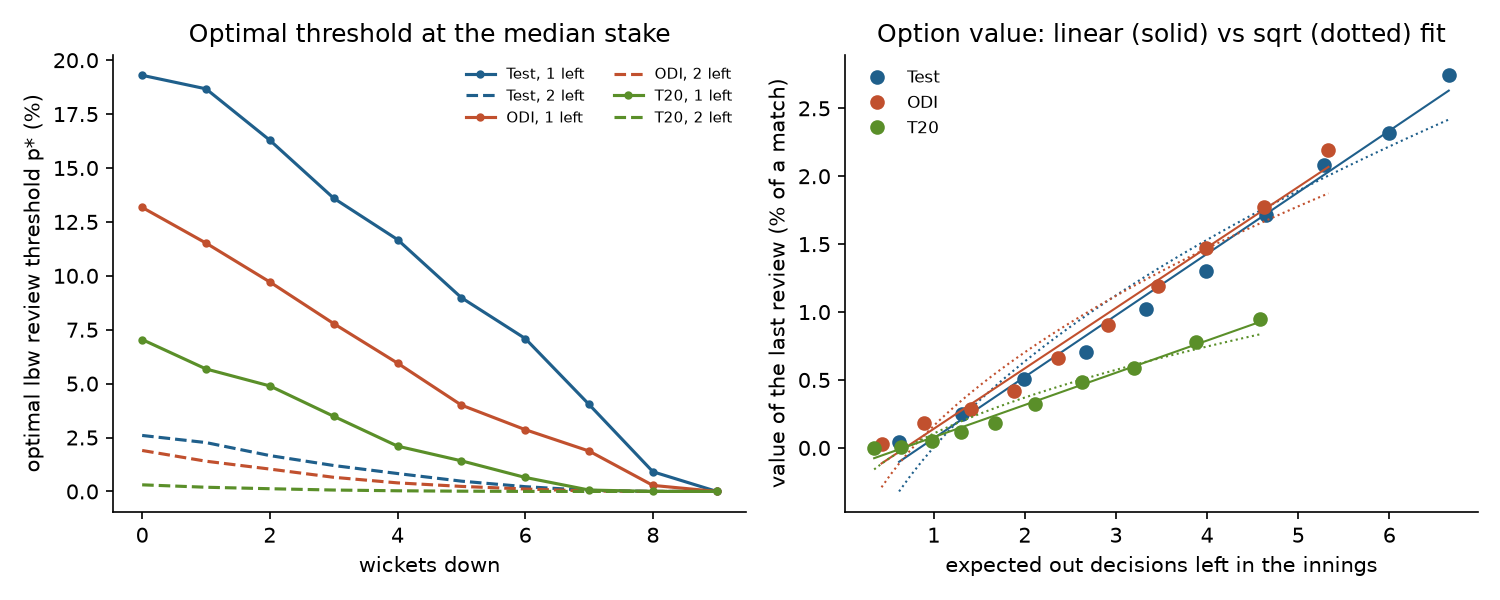
\includegraphics[width=.85\textwidth]{figures/fig_drs}
\caption{DRS, exploratory application, batting side, by format.}\label{fig:drs}
\end{figure}

Table~\ref{tab:drsthr} gives the optimal LBW threshold (posterior probability that the decision is wrong, in percent)
at each number of wickets down. With one review left it falls steadily from the top order to the tail; with two it is
near zero throughout. Table~\ref{tab:drssqrt} fits the value of the last review against the expected out decisions
left, $N$. A linear fit beats $\sqrt N$ in every format and the power exponent is well above $1/2$: with five to seven
out decisions per innings on average and about \DRSTestLBW\% of LBW out decisions wrong, the last review is worth
roughly the expected errors ahead times the stake. Exponents above one cannot come from the stationary model of
Theorem~\ref{thm:sqrtS}, where the increments $\Delta_t(1)-\Delta_{t-1}(1)=\varphi(\Delta_{t-1}(1))$ are
non-increasing (Lemma~\ref{lem:phi} with Theorem~\Mref{thm:mono}(b)) and growth is at most linear; they reflect stakes and decision rates that change with the wickets down. The square-root law is a statement
about a long stationary horizon whose confidence law has mass up to certainty with the tail of
Theorem~\ref{thm:sqrtS}; a batting innings, with a handful of decisions whose stakes change with the wickets down, is
far from that regime.

\begin{table}[!htbp]
\caption{Optimal LBW review threshold (\%) by wickets down and reviews left.}\label{tab:drsthr}
\centering\scriptsize
\resizebox{\textwidth}{!}{\begin{tabular}{lrrrrrrrrrr}
\toprule
Wickets down & 0 & 1 & 2 & 3 & 4 & 5 & 6 & 7 & 8 & 9 \\
\midrule
Test, 1 left & 19.3 & 18.7 & 16.3 & 13.6 & 11.7 & 9.0 & 7.1 & 4.0 & 0.9 & 0.0 \\
Test, 2 left & 2.6 & 2.3 & 1.7 & 1.2 & 0.8 & 0.5 & 0.2 & 0.0 & 0.0 & 0.0 \\
ODI, 1 left & 13.2 & 11.5 & 9.7 & 7.8 & 6.0 & 4.0 & 2.9 & 1.9 & 0.3 & 0.0 \\
ODI, 2 left & 1.9 & 1.4 & 1.0 & 0.7 & 0.4 & 0.2 & 0.1 & 0.0 & 0.0 & 0.0 \\
T20, 1 left & 7.0 & 5.7 & 4.9 & 3.5 & 2.1 & 1.4 & 0.6 & 0.1 & 0.0 & 0.0 \\
T20, 2 left & 0.3 & 0.2 & 0.1 & 0.1 & 0.0 & 0.0 & 0.0 & 0.0 & 0.0 & 0.0 \\
\bottomrule
\end{tabular}
}
\end{table}

\begin{table}[!htbp]
\caption{Value of the last review against the out decisions left.}\label{tab:drssqrt}
\centering\small
\resizebox{\textwidth}{!}{\begin{tabular}{lrrr}
\toprule
 & Test & ODI & T20 \\
\midrule
$R^2$ of $\Delta_1$ on $\sqrt N$ & 0.940 & 0.923 & 0.934 \\
$R^2$ of $\Delta_1$ on $N$ & 0.989 & 0.985 & 0.988 \\
Power exponent [95\% CI] & 1.66 [1.51, 1.80] & 1.67 [1.49, 1.86] & 1.85 [1.57, 2.13] \\
Expected out decisions left at the start, $N$ & 6.65 & 5.33 & 4.58 \\
\bottomrule
\end{tabular}
}
\end{table}

\subsection{Sensitivity and limitations}
Table~\ref{tab:drssens} varies perception noise, the umpire's-call model, the WP engine and the stakes. Losses become
material only if perception is poor ($s=2$), which the likelihood rejects in Tests and T20 but not in ODIs, where the
no-loss conclusion rests on the point estimate of $s$. The one-line rule stays within a few percent of the benchmark in
every variant. On the fielding side only reviews are observed; not-out appeals that were not reviewed leave no trace,
so the opportunity set, the benchmark and the loss cannot be estimated. Descriptively, fielding reviews succeed in
\SDRSBowlTestSuccess, \SDRSBowlODISuccess{} and \SDRSBowlTtSuccess\% of cases (Test, ODI, T20) and end in umpire's call
in \SDRSBowlTestUC, \SDRSBowlODIUC{} and \SDRSBowlTtUC\%.

\begin{table}[!htbp]
\caption{DRS sensitivity, batting side: benchmark / lost vs fitted rule / one-line rule's share of the benchmark (\%), match
points per 100 team-matches. $-\Delta\ell$: profile log-likelihood loss of $s$.}\label{tab:drssens}
\centering\scriptsize
\resizebox{\textwidth}{!}{\begin{tabular}{lccc}
\toprule
 & Test & ODI & T20 \\
\midrule
Main (band model, $\hat s$) & 5.61 / 0.020 / 99.8 & 2.28 / 0.018 / 98.5 & 0.96 / 0.001 / 99.5 \\
Upper end of the $s$ set & 5.60 / 0.053 / 98.7 ($s=0.84$) & 2.94 / 0.724 / 93.9 ($s=2.28$) & 0.97 / 0.016 / 99.2 ($s=0.86$) \\
$s=2$ & 6.66 / 1.174 / 95.4 ($-\Delta\ell=5.21$) & 2.78 / 0.549 / 93.8 ($-\Delta\ell=1.57$) & 1.38 / 0.452 / 93.8 ($-\Delta\ell=4.46$) \\
Constant-rate umpire's call & 5.39 / 0.032 / 99.7 & 2.33 / 0.023 / 99.5 & 0.96 / 0.000 / 99.8 \\
Recalibrated WP engine & 5.70 / 0.022 / 99.8 & 2.32 / 0.017 / 98.5 & 1.01 / 0.002 / 99.4 \\
Stakes $\times1.5$ & 8.41 / 0.030 / 99.9 & 3.42 / 0.027 / 98.5 & 1.44 / 0.002 / 99.5 \\
Stakes $\times0.67$ & 3.76 / 0.013 / 99.9 & 1.53 / 0.012 / 98.3 & 0.64 / 0.001 / 99.6 \\
\bottomrule
\end{tabular}
}
\end{table}

\paragraph{Limitations} The WP engines are league-average, with no team strength or conditions. The Gaussian margin
model is parametric, and its shape beyond the observed thresholds is assumed. The DP pools stakes by wickets down, so
overs left and declarations enter only through the empirical rates. The counterfactual keeps the real decision stream
fixed: a batter reprieved in simulation creates no new decisions, the same approximation as the MLB path sum, and there
is no causal re-simulation for DRS; solving the DP without the extra opportunity after a successful review, so that
DP and evaluation share one process, moves the benchmark by at most a few thousandths of a match point. The best
$\delta$ chosen on one half of the matches by date and scored on the other keeps \SDRSCrossShareLo--\SDRSCrossShareHi\%
of the benchmark.

\bibliographystyle{spr-ims-nameyear}
\bibliography{refs}

\end{document}
